\documentclass[twoside,openright,titlepage,numbers=noenddot,headinclude,%
               footinclude=true,cleardoublepage=empty,abstractoff,BCOR=5mm,%
               paper=a4,fontsize=12pt]{book}

\usepackage[left=1.5in, right=1in, top=1.25in, bottom=1.25in]{geometry}

\usepackage{scrextend}  % for addmargin command
\usepackage{graphicx}
% subcaption package is for subfigure environment
\usepackage{subcaption}
\usepackage[usenames, dvipsnames]{color}

% bold greek letter
\usepackage{amsmath}
\usepackage{xspace}
\usepackage{bm}
\usepackage{bbold}

% To add line number
\usepackage{lineno}

% For feynman diagram


\usepackage{comment}

\usepackage{epigraph}

% for <bra> <ket> notation 
\usepackage{braket}


\usepackage{textcomp}

% for degree symbol (https://tex.stackexchange.com/questions/384873/what-is-the-degree-symbol)
\usepackage{siunitx}

% for highligted tables
\usepackage{tabularx}
\usepackage{colortbl}
\usepackage{hhline}

% Below 3 lines are added to behave footnote command as its normal form inside table environment.  Reference: https://tex.stackexchange.com/a/109471/41568
\usepackage{footnote}
\makesavenoteenv{tabular}
\makesavenoteenv{table}
\usepackage{multirow}


% packages for todonotes
\usepackage[colorlinks]{hyperref}
\usepackage[table]{xcolor}
% \usepackage[colorinlistoftodos]{todonotes}
\usepackage[disable]{todonotes} % To hide uncomment this and comment upper line
% \usepackage{menukeys}

\usepackage{url}

\usepackage[backend=bibtex,style=numeric,sorting=none]{biblatex}
\addbibresource{ThesisBibliography.bib}


\usepackage{imakeidx}
\makeindex

\usepackage[acronym,toc,nomain,nonumberlist]{glossaries}
\makeglossaries

\usepackage[toc,page]{appendix}
%
%	define all acronyms
%
\newacronym{sm}{SM}{Standard Model}
\newacronym{lhc}{LHC}{Large Hadron Collider}
\newacronym{hep}{HEP}{High Energy Physics}

\usepackage{setspace}
 
% \onehalfspacing
\doublespacing

% How to make curvy L
% Reference: https://tex.stackexchange.com/a/11144/41568
% arrow
\newcommand{\To}{\ensuremath{\rightarrow}}
% \newcommand{\to}{\ensuremath{\rightarrow}}

\newcommand{\bT}{\boldsymbol{T}}
\newcommand{\bt}{\boldsymbol{T}}
\newcommand{\bw}{\boldsymbol{W}}
\newcommand{\bW}{\boldsymbol{W}}
\newcommand{\w}{\boldsymbol{W}}
\newcommand{\z}{\boldsymbol{Z}}
\newcommand{\Z}{\boldsymbol{Z}}
% \newcommand{\W}{\boldsymbol{W}}
\newcommand{\bsigma}{\boldsymbol{\sigma}}
\newcommand{\Lagr}{\mathcal{L}}
\newcommand{\Oo}{\mathcal{O}}
\newcommand{\Et}{\ensuremath{E_\mathrm{T}}}
\newcommand{\Pt}{\ensuremath{P_\mathrm{T}}}
\newcommand{\pt}{\ensuremath{P_\mathrm{T}}}
\newcommand{\met}{\ensuremath{\Et^{\mathrm{miss}}}}
\newcommand{\ptmiss}{\ensuremath{\Pt^{\mathrm{miss}}}}
\newcommand{\Ptmiss}{\ensuremath{\Pt^{\mathrm{miss}}}}
% \newcommand{\WW}{\ensuremath{\bW^+\bW^-}}
\newcommand{\ww}{\ensuremath{\bW^+\bW^-}}
% \newcommand{\zz}{\ensuremath{\Z \Z}}
\newcommand{\WWj}{\ensuremath{\bW^+\bW^-jj}}
\newcommand{\wwj}{\ensuremath{\bW^+\bW^-jj}}
% \newcommand{\Wjets}{\ensuremath{\mathrm{W+jets}}}
% \newcommand{\Zjets}{\ensuremath{\mathrm{Z+jets}}}
\newcommand{\GeV}{\ensuremath{\mathrm{GeV}}}
\newcommand{\PV}{\ensuremath{\mathrm{V}}}
\newcommand{\PW}{\ensuremath{\mathrm{W}}}
\newcommand{\PZ}{\ensuremath{\mathrm{Z}}}
\newcommand{\TeV}{\ensuremath{\mathrm{TeV}}}
\newcommand{\tev}{\ensuremath{\mathrm{TeV}}}
\newcommand{\ifb}{\ensuremath{\mathrm{fb^{-1}}}}
\newcommand{\fbinv}{\ensuremath{\mathrm{fb^{-1}}}}
\newcommand{\PHpm}{\ensuremath{\mathrm{H}^{\pm}}}
\newcommand{\PH}{\ensuremath{\mathrm{H}}}
\newcommand{\MADGRAPH}{\textsc{MadGraph}}
\newcommand{\MCATNLO}{\textsc{mc}\ensuremath{@}\textsc{nlo}}
\newcommand{\balpha}{\boldsymbol{\alpha(x)}}
\newcommand{\ttbar}{\ensuremath{t\bar{t}}}
\newcommand{\PYTHIA}{\textsc{pythiya}}
\newcommand{\kt}{\ensuremath{k_\mathrm{T}}}
% Some shorthand
% turn off italics
\newcommand{\etal}{\mbox{et al.}\xspace} %et al. - no preceding comma
\newcommand{\ie}{\mbox{i.e.}\xspace}     %i.e.
\newcommand{\eg}{\mbox{e.g.}\xspace}     %e.g.
\newcommand{\etc}{\mbox{etc.}\xspace}     %etc.
\newcommand{\vs}{\mbox{\sl vs.}\xspace}      %vs.
\newcommand{\mdash}{\ensuremath{\mathrm{-}}} % for use within formulas
\providecommand {\NA}{\ensuremath{\text{---}}}    % for Not applicable (or available). Needs to be renewcommanded for APS to \cdots

% some terms whose definition we may change
\newcommand{\Lone}{Level-1\xspace} % Level-1 or L1 ?
\newcommand{\Ltwo}{Level-2\xspace}
\newcommand{\Lthree}{Level-3\xspace}

% processes
\newcommand{\dyee}{\ensuremath{Z/\gamma^*\to e^+e^-}}
\newcommand{\dymm}{\ensuremath{Z/\gamma^*\to\mu^+\mu^-}}
\newcommand{\dytt}{\ensuremath{Z/\gamma^*\to\tau^+\tau^-}}
\newcommand{\dyll}{\ensuremath{Z/\gamma^*\to\ell^+\ell^-}}
\newcommand{\zee}{\ensuremath{Z\to e^+e^-}}
\newcommand{\zmm}{\ensuremath{Z\to\mu^+\mu^-}}
\newcommand{\ztt}{\ensuremath{Z\to\tau^+\tau^-}}
\newcommand{\zll}{\ensuremath{Z\to\ell^+\ell^-}}
%\newcommand{\ttbar}{\ensuremath{t\bar{t}}}
\newcommand{\ppww}{\ensuremath{pp \to W^+W^-}}
\newcommand{\wwll}{\ensuremath{WW\to \ell^+\ell^-}}
\newcommand{\wwlnln}{\ensuremath{W^+W^-\to \ell^+\nu \ell^-\bar{\nu}}}
\newcommand{\hww}{\ensuremath{\Hi \to \WW}}
\newcommand{\wz}{\ensuremath{WZ}}
\newcommand{\zz}{\ensuremath{ZZ}}
\newcommand{\wgamma}{\ensuremath{W\gamma}}
\newcommand{\wjets}{\ensuremath{W+}jets} 
\newcommand{\tw}{\ensuremath{tW}} 
\newcommand{\singletopt}{\ensuremath{t} ($t$-chan)} 
\newcommand{\singletops}{\ensuremath{t} ($s$-chan)} 
\newcommand{\cPZ}{\PZ} % plain Z (no superscript 0)

% particles

\newcommand{\pipm}{\ensuremath{\pi^{\pm}}}
\newcommand{\pizero}{\ensuremath{\pi^{0}}}
\newcommand{\Hi}{\ensuremath{\mathrm{H}}}
\newcommand{\V}{\ensuremath{\mathrm{V}}}
\newcommand{\W}{\ensuremath{\mathrm{W}}}
\newcommand{\Wjets}{\ensuremath{\mathrm{W+jets}}}
\newcommand{\Zjets}{\ensuremath{\mathrm{Z+jets}}}
\newcommand{\Wt}{\ensuremath{\mathrm{Wt}}}
\newcommand{\Wstar}{\ensuremath{\mathrm{W}^{*}}}
\newcommand{\Wparenthesisstar}{\ensuremath{\mathrm{W}^{(*)}}}
\newcommand{\WW}{\ensuremath{\W^+\W^-}}
\newcommand{\PHpmpm}{\ensuremath{\mathrm{H^{\pm\pm}}}}
%\newcommand{\Z}{\ensuremath{\mathrm{Z}}}
\newcommand{\Zstar}{\ensuremath{\mathrm{Z}^{*}}}
\newcommand{\ZZ}{\ensuremath{\Z\Z}}
\newcommand{\WZ}{\ensuremath{\W\Z}}
\newcommand{\El}{\ensuremath{\mathrm{e}}}
\newcommand{\Elp}{\ensuremath{\mathrm{e}^{+}}}
\newcommand{\Elm}{\ensuremath{\mathrm{e}^{-}}}
\newcommand{\Elpm}{\ensuremath{\mathrm{e}^{\pm}}}
\newcommand{\Elmp}{\ensuremath{\mathrm{e}^{\mp}}}
\newcommand{\M}{\ensuremath{\mu}}
\newcommand{\Mp}{\ensuremath{\mu^{+}}}
\newcommand{\Mm}{\ensuremath{\mu^{-}}}
\newcommand{\Mpm}{\ensuremath{\mu^{\pm}}}
\newcommand{\Mmp}{\ensuremath{\mu^{\mp}}}
\newcommand{\Tau}{\ensuremath{\tau}}
\newcommand{\Nu}{\ensuremath{\nu}}
\newcommand{\Nubar}{\ensuremath{\bar{\nu}}}
\newcommand{\Lep}{\ensuremath{\ell}}
\newcommand{\Lepp}{\ensuremath{\ell^{+}}}
\newcommand{\Lepm}{\ensuremath{\ell^{-}}}
\newcommand{\Lprime}{\ensuremath{\Lep^{\prime}}}
\newcommand{\Prot}{\ensuremath{\mathrm{p}}}
\newcommand{\Pbar}{\ensuremath{\bar{\mathrm{p}}}}
\newcommand{\PP}{\Prot\Prot}
\newcommand{\PPbar}{\Prot\Pbar}
%\newcommand{\ttbar}{\ensuremath{\mathrm{t}\bar{\mathrm{t}}}}
\newcommand{\qq}{\ensuremath{\mathrm{q}\mathrm{q}}}
%\newcommand{\bbbar}{\ensuremath{\mathrm{b}\bar{\mathrm{b}}}}
\newcommand{\Wtb}{\ensuremath{\W\mathrm{t}\mathrm{b}}}
\newcommand{\Top}{\ensuremath{\mathrm{t}}}
\newcommand{\Bot}{\ensuremath{\mathrm{b}}}
\newcommand{\Atop}{\ensuremath{\bar{\mathrm{t}}}}
\newcommand{\Abot}{\ensuremath{\bar{\mathrm{b}}}}
\newcommand{\WH}{\ensuremath{\W\Hi}}
\newcommand{\ZH}{\ensuremath{\Z\Hi}}


% \newenvironment{scotch}[1]{\protect\centering\ruledtabular\tabular{#1}}{\endtabular\endruledtabular}
\newenvironment{scotch}[1]{\protect\centering\tabular{#1}\hline\hline}{\hline\endtabular}

\makeatletter
\renewcommand{\@chapapp}{}% Not necessary...
\newenvironment{chapquote}[2][2em]
  {\setlength{\@tempdima}{#1}%
   \def\chapquote@author{#2}%
   \parshape 1 \@tempdima \dimexpr\textwidth-2\@tempdima\relax%
   \itshape}
  {\par\normalfont\hfill--\ \chapquote@author\hspace*{\@tempdima}\par\bigskip}
\makeatother

\begin{document}
 % \linenumbers
 \pagenumbering{roman}
 \pagestyle{plain}

% Front pages =================================================================
 % \begin{titlepage}
	\begin{addmargin}[-1cm]{-1cm}
    \begin{center}
        \large
    \includegraphics[width=0.35\textwidth]{figures/logo_du.jpg}\\
        \vfill
        {\Large \textsc{University of Delhi}}\\[1ex]
        Department of Physics \& Astrophysics\\

        \vfill

        PhD Thesis\\ \vskip1cm
        \rule{14cm}{0.4pt} \\ \bigskip
        % \begingroup
            % \Large
            \textbf{\Large{\color{Maroon}{Search for Anomalous Gauge Coupling through Vector Boson Scattering and Development of the GEM Detectors at the CMS Experiment}}} \\ \bigskip
            % \textbf{\Large{\color{Maroon}{Search for Anomalous Gauge Coupling through Vector Boson Scattering with the CMS Experiment at the LHC and Development of the GEM Detectors for Muon System}}} \\ \bigskip
            % \textbf{\Large{\color{Maroon}{Search for Anomalous Gauge Coupling with Vector Boson Scattering at the CMS Experiment and Development of the GEM Detectors for Muon System}}} \\ \bigskip
            % \textbf{\Large{\color{Maroon}{Search for Anomalous Gauge Coupling with VBS at the CMS Experiment and Development of the GEM Detectors for Muon System}}} \\ \bigskip
            % \textbf{\Large{\color{Maroon}{Search for Anomalous Gauge Coupling in VV VBF Channel at the CMS Experiment and Development of the GEM Detectors for Muon System}}} \\ \bigskip
            % \textbf{\Large{\color{Maroon}{Search for Anomalous Gauge Coupling in VV VBF Channel at the CMS Experiment and Development of the GEM Detectors for Muon System}}} \\ \bigskip


            % \textbf{{\color{Maroon}{{\LARGE{S}}earch for {\LARGE{aQGC}} in {\LARGE{WW}} {\LARGE{VBF}} {\LARGE{C}}hannel at the {\LARGE{CMS}} {\LARGE{E}}xperiment and {\LARGE{D}}evelopment of the {\LARGE{GEM}} {\LARGE{D}}etectors for {\LARGE{M}}uon {\LARGE{S}}ystem}}} \\ \bigskip
            % \textbf{\Large{\color{Maroon}{Search for aQGC in WW VBF Channel at the CMS Experiment and Development of the GEM Detectors for Muon System}}} \\ \bigskip
            % {\color{Maroon}{{\LARGE{S}}EARCH {\LARGE{F}}OR {\LARGE{aQGC}} IN {\LARGE{WW}} VBF {\LARGE{C}}HANNEL AT THE CMS {\LARGE{E}}XPERIMENT AND {\LARGE{D}}EVELOPMENT OF GEM {\LARGE{D}}ETECTORS {\LARGE{F}}OR {\LARGE{M}}UON {\LARGE{S}}YSTEM {\LARGE{U}}PGRADE}} \\ \bigskip
            % {\color{Maroon}{{\LARGE{S}}EARCH {\LARGE{F}}OR {\LARGE{N}}EW {\LARGE{P}}HENOMENA {\LARGE{I}}N {\LARGE{H}}IGH {\LARGE{E}}NERGY {\LARGE{I}}NTERACTIONS}} \\ \bigskip
            % \color{Maroon}\spacedallcaps{\myTitle} \\ \bigskip
        % \endgroup
        %\spacedlowsmallcaps{\mySubtitle} \\ \bigskip
        \rule{14cm}{0.4pt}\\ \vskip1cm
        by \textsc{Ram Krishna Sharma}\\
        \vfill
        Advisor: Dr. \textsc{Md. Naimuddin}\\

        \vfill
        \vfill
        \vfill

        %\hfill April 2017
    \end{center}
  \end{addmargin}
\end{titlepage}
 \listoftodos
  % \cleardoublepage \begin{center}
\textbf{\LARGE Declaration}
\end{center}
\vspace{1.5cm}
This thesis describes work done by the candidate during his tenure as Ph.D. student at the Department of Physics and Astrophysics, University of Delhi, Delhi, India under the supervision of Dr. Md. Naimuddin. The work reported in this thesis is original and it has not been submitted earlier for any degree to any university. 
\vfill
{\flushleft Candidate} \hspace{4cm} \dotfill \\
{\flushright {\textbf{Ram Krishna Sharma}}}

\vfill
{\flushleft Supervisor} \hspace{4cm} \dotfill \\
{\flushright{\textbf{Dr. Md. Naimuddin}}}

\vfill
{\flushleft Head of Department} \hspace{2.5cm} \dotfill \\
{\flushright {\textbf{Prof. Sanjay Jain}}}
\vfill
  % \cleardoublepage %\vspace{1.5cm}
%
\begin{tabular}{l}
\includegraphics[scale=0.7]{figures/logo_du.jpg}
\end{tabular}
%
\hspace{3cm}
\begin{tabular}{r}
 \\
 \\
\color{blue} \textbf{Department of Physics  and Astrophysics} \\
 \\
\textbf{University of Delhi} \\
 \\
\textbf{Delhi-110007, India} \\
 \\
 \\
 \\
 \\
Date: ...................................  
\end{tabular}
%
\vspace{4cm}
\begin{center}
\textbf{\LARGE Certificate of Originality}
\end{center}
\vspace{1.5cm}
%
The research work embodied in this thesis entitled~``\textbf{Search For New Phenomena In High Energy Interactions}'' has been carried out by me at the \textbf{Department of Physics and Astrophysics}, University of Delhi, Delhi, India. The manuscript has been subjected to plagiarism check by \textbf{Turnitin} software. The work submitted for consideration of award of Ph.D. is original. \\
\begin{tabular}{cc}
 & \\
 & \\
 & \\
 & \\
 & \\
 & \hspace{9cm} ............................................................. \\
 & \hspace{9cm} \textbf{Ram Krishna Sharma} \\
 & \hspace{8.5cm} Name and Signature of the Candidate
\end{tabular}
  % \cleardoublepage \begin{center}
\textbf{\LARGE Student Approval Form}
\end{center}
\vspace{1cm}
%
%
%
\begin{tabular}{|l|p{12cm}|} \hline
 & \\ [-1em]
Name of the Author & {\bf Ram Krishna Sharma}\\ \hline
 & \\ [-1em]
Department & Department of Physics and Astrophysics\\ \hline
 & \\ [-1em]
Degree &  Doctor of Philosophy \\ \hline
 & \\ [-1em]
University & University of Delhi \\ \hline
 & \\ [-1em]
Guide & Dr. Md. Naimuddin \\ \hline
 & \\ [-1em]
Thesis Title & Search for anomalous gauge coupling through vector boson scattering and development of the GEM detectors at the CMS experiment\\ \hline
 & \\ [-1em]
Year of Award & \\ \hline
\end{tabular}
%
%
%
\vspace{0.5cm}
%
%
%
\begin{center}
\textbf{Agreement} \\
\end{center}
\vspace{0.5cm}
\begin{enumerate}
\item I hereby certify that if appropriate, I have obtained and attached hereto a written permission/statement from the owner(s) of each third party copyrighted matter to be included in my thesis/dissertation, allowing distribution as specified below.
\item I hereby grant to the university and its agents the non-exclusive license to archive and make accessible, under the conditions specified below, my thesis/dissertation, in whole or in part in all forms of media, now or hereafter known. I retain all other ownership rights to the copyright of the thesis/dissertation. I also retain the right to use in future works (such as articles or books) all or part of this thesis, dissertation, or project report.
\end{enumerate}
% \vspace{0.5cm}
%
%
%
\textbf{Conditions:} 
% \vspace{1cm}
\begin{tabular}{|p{10cm}|p{5cm}|} \hline
 & \\ [-1em]
1. Release the entire work for access worldwide & \\ \hline
 & \\ [-1em]
2. Release the entire work for \lq My University\rq only for: & \\ 
~\hspace{2cm}~\begin{tabular} {c} 1 Year \\ 2 Year \\ 3 Year \end{tabular} &  \\ 
and after this time release the work for access worldwide. &  \\ \hline
 & \\ [-1em]
  & \\ \hline
 % & \\ [-1em]
 3. Release the entire work for \lq My University\rq  only while at the same time releasing the following parts of the work (e.g. because other parts relate to publications) for worldwide access: &  \\
\begin{enumerate} \item[a)] Bibliographic details and Synopsis only \item[b)] Bibliographic details, synopsis and the following chapters only \item[c)] Preview/Table of Contents/24 page only \end{enumerate} & \\ \hline
 & \\ [-1em]
4. View Only (No Downloads) (worldwide) & \\ \hline
\end{tabular}

  % \cleardoublepage \begin{tabular}{|p{10cm}|p{5cm}|}
 & \\ \hline
 & \\ [-1em]
 3. Release the entire work for \lq My University\rq  only while at the same time releasing the following parts of the work (e.g. because other parts relate to publications) for worldwide access: &  \\
\begin{enumerate} \item[a)] Bibliographic details and Synopsis only \item[b)] Bibliographic details, synopsis and the following chapters only \item[c)] Preview/Table of Contents/24 page only \end{enumerate} & \\ \hline
 & \\ [-1em]
4. View Only (No Downloads) (worldwide) & \\ \hline
\end{tabular}
%
%
%
\begin{tabular}{c}
 \\
 \\
 \\
\end{tabular}
%
%
%
\begin{tabular}{p{7cm}p{8cm}}
 & \\
 & \\
 & \\
 & \\
 & \\
 & \\
 & \\
 & \\
 & \\
........................................... & \hspace{2cm} ....................................................... \\
Signature of the Scholar & \hspace{2cm} Signature and seal of the Guide \\
 & \\
 & \\
 & \\
Place: ......................... & \\
 & \\
 & \\
Date: ......................... &
\end{tabular}

  % \cleardoublepage \begin{center}
\vspace*{6cm}
\Huge
	\textbf{\textit{Dedicated To \\My Loving Parents }}
\end{center}
  % \cleardoublepage % Acknowledgements ============================================================

%\pdfbookmark[1]{Acknowledgments}{acknowledgments}
\chapter*{Acknowledgments}

As the saying goes, good premises do not entail good stories. 
  % \cleardoublepage %\pdfbookmark[1]{Abstract}{Abstract}
\chapter*{Abstract}
In the Standard Model (SM) of particle physics, masses for the particles are generated by the Higgs mechanism, which requires the existence of a spin-0 particle called the Higgs boson. In July 2012, a new Higgs like particle is discovered with mass 125-126 GeV at the LHC. This may be the long sought Higgs boson of the standard model (SM), which was proposed in 1960s, or one of the Higgs bosons beyond the SM. For example, super-symmetric theories, little-Higgs models, and other extended Higgs sector such as the Georgi-Machacek model all contain a multitude of neutral as well as charged Higgs bosons. Because, the current data still contain large uncertainties that these various extensions of the SM cannot be confirmed or ruled out decisively. So, It is important to at-least constraint the various couplings of the Higgs boson, based on the signal strength of all decay channels of the Higgs boson. One of the most useful constraints from the global fitting of the Higgs boson couplings is the one to a pair of W/Z bosons.
% The current data constrain
% 	\begin{equation}
% 	C_v = \frac{g_{hWW}}{g_{hWW}^{SM}} = 0.96^{+0.13}_{-0.15}
% 	\end{equation}
% The central value is close to 1, which means that the observed Higgs boson leaves only little room for the existence of another Higgs boson or some unknown unitarity violation (UV) physics responsible for the electroweak symmetry breaking (EWSB). If $C_v$ is exactly equal to 1, it means that the observed Higgs boson will completely account for the EWSB. We do not need another Higgs boson, or if it exists it has nothing to do with the EWSB.

% If the hWW coupling is less than its SM value, there must be something heavier, could be as heavy as a few TeV, to complete the EWSB. 
% In particular, through proton-proton collisions it is expected to shed light on the mechanism responsible for electroweak symmetry breaking. 

% In the SM of particle physics, masses for the particles are generated by the Higgs mechanism, which requires the existence of a spin-0 particle called the Higgs boson. This particle is discovered now at approx. 125 GeV but it is not sure that it is the Higgs boson which is responsible for the EWSB.

% It is possible that the Higgs boson does not exist. In the SM without Higgs boson, the tree level amplitude for longitudinal vector boson scattering $V_LV_L\rightarrow V_LV_L$ violates unitarity at a centre-of-mass energy of 1.2 TeV. New physics, perhaps accompanied by new particles, must appear at or before this scale. It will therefore be crucial to measure vector boson (W or Z) scattering up to the highest possible energies either as a search for the new physics or as confirmation that our understanding of any new physics found in other channels is correct.

  \pagestyle{headings}
  \cleardoublepage%\include{frontback/toc}
   \tableofcontents 
   % \listoffigures 
   % \listoftables
  % Content =====================================================================
  \cleardoublepage
  \pagenumbering{arabic}
  % \chapter{Introduction}
\begin{chapquote}
{Edward Witten}
``Particle physics is a modern name for the centuries old effort to understand the basic laws of physics.''
\end{chapquote}
Ever since its existence mankind is striving to unravel mysteries of Nature around us. Several theoretical frameworks have been developed to answer key questions regarding our existence on this planet.  Continuous endeavours of the scientists in this regard lead to the evolution of a branch of physics, namely ``\textit{particle physics}'', dealing with the study of fundamental particles and the interactions among them. 

Standard Model (SM) of particle physics is a theoretical framework, developed in the 1960s and 70s, which encapsulates our current understandings about the particles and their interactions.
SM has been very successful in predicting the behaviour and certain characteristics of the elementary particles. It gives a compelling explanation of the existing experimental data.
The only missing link, the long sought after Higgs boson, was found in 2012 at the CERN Large Hadron Collider (LHC), and its properties were measured in the following years, thus completing the picture of elementary particles predicted by the SM.
However, the SM still leaves some unexplained phenomena, such as neutrino oscillations, the reason behind the spontaneous symmetry breaking which is responsible for the mass generation to the elementary particles and solves that unitarity problem in vector-boson scattering, baryon asymmetry, why there is mass hierarchy?
After the discovery of Higgs Boson, the major goal of the physics programme at the LHC is to provide a definitive answer to these open questions by significantly expanding both the energy reach and the collision rate with respect to 
the previous experiments and its own Run periods.
Now, one of important task is to investigate the possible structure of the $SU(2)\times U(1)$-breaking physics and its experimental signature. These includes the precision measurement in the electroweak sector~\cite{Baak2013} and to look for the vector boson scattering.

	
As, the scattering of the vector bosons is strongly connected to electroweak symmetry breaking (EWSB) in the SM, regulated by the Brout-Englert-Higgs mechanism.
These electroweak gauge bosons acquire mass through the EWSB, turning the massless Goldstone bosons in their longitudinal polarization.
The recent discovery of the Higgs boson indicates that the ultimate EWSB should be similar to  the existing Higgs mechanism(ref).
The VBS process also contains information on the quartic vector boson interactions, a part of the SM which has not been well tested yet and could be modified by new physics.
Thus, the VBS  emerges as a strong candidate process to serve the two-fold purpose to perform the precision measurements and side-by-side look for the new physics phenomenon.  


This thesis is organized as follows. In Chapter-2, the brief introduction of the SM and the generation of triple or quartic gauge coupling in the SM followed with the brief introduction of the Higgs mechanism. As we know that for the study of the particle physics one need an accelerator and a detector that can accelerate the particles and collides them to probe the physics at small scale, which will help us to understand the behaviour and interaction of particles. Thus the briefly the one of largest accelerator Large Hadron Collider and its one of main purpose detectors design and working principle is explained in Chapter-3. Furthermore, one need to upgrade the detector with time to maintain the physics requirement. In this thesis one of sub-system upgrade details are mentioned in Chapter-4, which includes the test beam studies and the test and characterisation of the GEM foil performed at the University of Delhi. In Chapter-5, the physics studies of the anomalous quartic gauge coupling is given along with the doubly charged Higgs.
  % \chapter{Introduction} % (fold)
\label{cha:standard_model__vector_boson_scattering}
% \begin{chapquote}
% {C.N. Yang}
% Now if we adopt the view that this arbitrary convention should be independently chosen at every space-time point, then we are naturally led to the concept of gauge fields.
% \end{chapquote}

\begin{chapquote}
{Edward Witten}
``Particle physics is a modern name for the centuries old effort to understand the basic laws of physics.''
\end{chapquote}
Ever since the existence, mankind is striving to unravel mysteries of nature around us. Several theoretical frameworks have been developed to answer key questions regarding our existence in this Universe. Continuous endeavours of the thinkers and scientists in this regard lead to the evolution of a branch of physics, namely ``\textit{particle physics}'', dealing with the study of fundamental particles and the interactions amongst them. 

Standard Model (SM) of particle physics is a theoretical framework, developed in the 1960s and 70s, which encapsulates nearly all that is known about the elementary particles and forces in a concise set of principles and equations. SM has been very successful in predicting the behaviour and certain characteristics of the elementary particles. It gives a compelling explanation of the existing experimental data. During 1960’s, while trying to unify the theories of electromagnetic and weak interactions it was realized that gauge bosons mediating these interactions should be massless which was in contradiction with the  experimental evidences~\cite{StandardModel67_1,StandardModel67_2,StandardModel67_3,}. This dilemma was resolved by P.W. Higgs, F. Englert, R. Brout  and others, by postulating that  the electroweak gauge symmetry is spontaneously broken~\cite{Englert1964,Higgs1964,Higgs1964a,Guralnik1964,Higgs1966,Kibble1967}, which gives mass to the elementary particles and the force carriers but it requires  a new scalar (spin-zero) particle, namely the Higgs boson. This new scalar boson not only provides mass to the elementary particles but it solves other problems such as: it preserves the unitarity of the Vector-Boson Scattering (VBS). It was the only missing link from SM till 2012. In 2012, it was observed at the CERN Large Hadron Collider (LHC)~\cite{Chatrchyan:2012xdj,Aad:2012tfa}, and its properties were measured in the following years. This completes the picture of the elementary particles predicted by the SM. However, the SM still leaves some unexplained phenomena, such as: 
\begin{itemize}
    \item reason behind spontaneous symmetry breaking?
    \item Is the Higgs boson only source for preserving the unitrization in vector-boson scattering? 
    \item reason behind the baryon asymmetry in universe? and many more.
\end{itemize}
After the discovery of Higgs Boson, the major goal of the physics programme at the LHC is to provide a definitive answer to these open questions by significantly expanding both the energy reach and the collision rate with respect to the previous experiments and its own Run periods.
Ongoing measurements at the LHC also include the precision measurements in the electroweak sectors and to look for VBS which could also hint towards the existence of new physics phenomenon, indirectly~\cite{Baak2013}. These measurements could provide information on the structure of $SU(2) \times U(1)$-breaking physics and its experimental signatures. 
The scattering of the vector bosons is strongly connected to the electroweak symmetry breaking (EWSB) in the SM, regulated by the Brout-Englert-Higgs mechanism. This study will help one to clearly understand the role of the observed Higgs boson in the EWSB. Because Recent discovery of the Higgs boson indicates that the ultimate EWSB should be similar to the existing Higgs mechanism which needs to be scrutinized.

VBS processes can also provides information on the quartic vector boson interactions, a part of the SM which has not been tested yet and could be modified by the existence of new physics. Given the large amount of  high-luminosity data available at the LHC, it is possible to probe this rare physics process using different final states. Thus, the VBS  emerges as a strong candidate process to serve the two-fold purpose to perform the precision measurements and side-by-side look for the new physics phenomenon.  
In this chapter, a brief introduction of the SM along with the EWSB is given. Also, the anomalous quartic gauge coupling and VBS are discussed briefly along with the doubly charged Higgs model in the framework of model created by the Georgi and Machacek.

%%%%%%%%%%%%%%%%%%%%%%%%%%%%%%%%
%%%%%%%%%%%%%%%%%%%%%%%%%%%%%%%%
\section{Brief Introduction of SM} % (fold)
\label{sec:brief_introduction_of_sm}
SM is the theory of elementary particles and their interactions. It is well tested and in good agreement with experimental results, obtained so far.

Till now we know of four fundamental interactions.
Out of the four, the gravitational interaction is not included in SM.
The other three forces - the strong force interaction as described by Quantum Chromodynamics (QCD), the electromagnetic interaction as described by Quantum Electrodynamics (QED) and the weak interaction - are included in the SM.
In 1979, Sheldon Glashow, Abdus Salam, and Steven Weinberg were awarded Nobel prize for their effort to unify the theory of weak interaction and the quantum electrodynamics~\cite{StandardModel67_1,StandardModel67_2}.
This unified theory of weak interaction and quantum electrodynamics is known as the electroweak theory.

According to SM all the fundamental particles can be classified into two categories. They are fermions and bosons.

Fermions are the particles that obey the Fermi-Dirac statistics with half-integer spin.
In SM, fermions are further classified into leptons and quarks, which are listed in Table~\ref{table:smfermions}.
The quarks and leptons create the subatomic scaffolding for solid matter.
Quarks bind together to form protons and neutrons and the electrons orbit these cluster of quarks to form atoms and the atoms combine into all the known stable matter of universe~\cite{SM-buildingblock_uslhc}.
Till now we know the three generations of leptons as well as quarks. The different generations are differing only in the particle mass.
\begin{table}
% \vspace{-5.2em}
\centering
{\small
\begin{tabular}[!htbp]{l l l l l l}
\hline
{\textbf{Generation}} & {\textbf{Fermion}} & {\textbf{Electric}} & \multicolumn{2}{c}{\textbf{Weak isospin $|I_3|$}} & \textbf{Mass in MeV} \\
    &           &    \textbf{Charge}  & \textbf{left-} & \textbf{right-} &     \\
    &           &                     & \textbf{handed} & \textbf{handed} &    \\
\hline
\multirow{4}{*}{$1^{st}$} & electron ($e^-$)           &   -1 & 1/2 &  0    &   $0.511\pm 3.1\times 10^{-8}$ \\
         & electron-neutrino ($\nu_e$)&   0  & 1/2 &  none &   $<2 \times 10^{-6}$   \\
         & up quark ($u$)             &  2/3 & 1/2 &  0    &   $2.2^{+0.5}_{-0.4}$  \\
         & down quark ($d$)           & -1/3 & 1/2 &  0    &   $4.7^{+0.5}_{-0.3}$  \\
\hline
\multirow{4}{*}{$2^{nd}$} & muon ($\mu^-$)             &  -1  & 1/2 &  0    &   $105.658 \pm 2.4 \times 10^{-6}$ \\
         & muon-neutrino ($\nu_{\mu}$)& 0    & 1/2 &  none &   $<2 \times 10^{-6}$   \\
         & charm quark ($c$)                & 2/3  & 1/2 &  0    &   $1275^{+25}_{-35}$     \\
         & strange quark ($s$)              & -1/3 & 1/2 &  0    &   $95^{+9}_{-3}$       \\
\hline
\multirow{4}{*}{$3^{rd}$} & tau ($\tau^-$)             & -1   & 1/2 &  0    &    1776.86 $\pm$ 0.12    \\
         & tau-neutrino ($\tau_{\mu}$)& 0    & 1/2 &  none &   $<2 \times 10^{-6}$   \\
         & top quark ($t$)                  & 2/3  & 1/2 &  0    &   $1.73\times 10^5\pm 40$\\
         & bottom quark ($b$)               & -1/3 & 1/2 &  0    &   ${4.18 \times 10^{3}}^{+40}_{-30}$\\
\hline
\end{tabular}
\caption{Fermions list in SM~\cite{PDG2018}.}
\label{table:smfermions}
}
\end{table}

Bosons are the particles that obey the Bose-Einstein statistics with integer spin. In SM the bosons are the mediator of interactions between the particles, described by a local gauge theory. Thus, these bosons are called gauge bosons. All the bosons in SM are listed in Table~\ref{table:smbosons}.
The photon and gluons are massless carrying electromagnetic and strong force respectively. The $W^{\pm}$ and $Z$ bosons carry the weak force. These bosons are the spin 1 bosons and known as the vector-bosons. Whereas, the Higgs boson, H, is a scalar boson with spin 0. This is responsible for the mass generation (by giving longitudinal polarization) to the fundamental particles through EWSB, which is explained in section~\ref{sub:brief_introduction_to_higgs_mechanism}.

\begin{table}
% \vspace{-5.2em}
{\small
\centering
\begin{tabular}[!htbp]{l l l l l l}
\hline
    & \textbf{Bosons} & \textbf{Electric Charge} & \textbf{Spin} & \textbf{Interaction} & \textbf{Mass in GeV} \\
\hline
$\gamma$  & photon   & 0      & 1 & electromagnetic   &   $<1 \times 10^{-27}$ \\
$W^{\pm}$ & W bosons & $\pm$1 & 1 & weak              &  80.379 $\pm$ 0.012    \\
$Z^0$     & Z boson  & 0      & 1 & weak              &  91.188 $\pm$ 0.0023    \\
$g$       & gluons   & 0      & 1 & strong            &  0                     \\
\hline
$H$       & Higgs    & 0      & 0 &                    & 125.18 $\pm$ 0.16     \\
\hline
\end{tabular}
\caption{Bosons list in SM~\cite{PDG2018}.}
\label{table:smbosons}
}
\end{table}

\subsection{Standard Model as Gauge theory}
Gauge invariance is the key ingredient in the construction of the SM of electromagnetic, weak and strong interactions of elementary particles. In general gauge principle specifies that for a given gauge symmetry group and the transformation of the fields, the quantum field theory can be uniquely defined~\cite{Coughlan2006}.
% Below the theory of Quantum Electrodynamics (QED) is briefly discussed.

% \subsubsection{Example: Quantum Electrodynamics} % (fold)
% \label{ssub:example_quantum_electrodynamics}
The construction of QED is an example of local gauge theory as the Lagrangian function (Eq.~\ref{eq:qed_lagrangian}) that describes the QED of the spin-half particle remains invariant by the local gauge transformation of the electron field $\psi(x)$ and the photon field $A_{\mu(x)}$ at all space-time point x,
\begin{equation}\label{eq:qed_lagrangian}
    \Lagr = i \bar{\psi}\gamma^{\mu} D_{\mu}\psi - m\bar{\psi}\psi,
    % \Lagr = i \bar{\psi}\gamma^{\mu} \partial_{\mu}\psi - m\bar{\psi}\psi
\end{equation}
The transformation followed by the electron field and photon field is:
\begin{eqnarray}\label{eq:qed_phase}
    \psi(x) & \rightarrow & e^{iq\chi(x)}\psi(x), \nonumber \\
    A_\mu(x) & \rightarrow & A_\mu(x) - {\partial_\mu \chi(x)}. 
\end{eqnarray}
Where the $\chi(x)$ is the arbitrary phase transformation, q is the electron-photon coupling.
And the $D_{\mu}$ given in the eq.~\ref{eq:qed_lagrangian} is known as covariant derivative and is given as:
\begin{equation}
    D_{\mu} = \partial_{\mu} + iqA_{\mu}.
\end{equation}
Here, the photon field plays an intrinsic role without which there could be no local gauge invariance. In the construction of the local gauge invariance of QED, we realize that the local gauge invariance of a spin-half particle requires the existence of a gauge boson and their coupling with the fermions. Also, for the exact gauge invariance, the gauge bosons must be massless. 

In Eq.~\ref{eq:qed_phase}, the phase factor $e^{i\chi(x)}$ belongs to the symmetry group $U(1)$ of the unitarity transformations in one dimension. Thus, the generalization of the QED can be made to the other forces by exploring other possibilities of the symmetry group.

For example, the electrons and neutrino can be chosen as a double $(\nu_e,e)$, i.e. as two members of the same family, since both of them are spin-half particles.
Thus, it can be described as the doublet by a two-component field $\phi = (\nu_e(x),e(x))$ and imposes a gauge transformation where $\alpha$ is a $2\times 2$ hermitian matrix operating on the $\phi$.

% \subsubsection{Example: Weak Interactions} % (fold)
% \label{ssub:example_weak_interactions}
The weak interaction, SU(2), local gauge transformation can be written for the electron doublet field as
\begin{eqnarray}
    \phi (x) &  = & e^{ig_w \balpha .\boldsymbol{T}} \phi(x) \nonumber \\
             &  \simeq & (I + ig_w \balpha \boldsymbol{.T})\phi(x),
\end{eqnarray}
where $\balpha$ is the arbitrary infinitesimal vector in the isospin space and the $\bt = \{T_1,T_2,T_3\}$ is the three generators of the SU(2) symmetry group, which can be expressed using Pauli spin matrices as $\bt = \bsigma / 2$. Also, the $\bt_i$ do not commute,\begin{equation}
    [T_i,T_j] = i\epsilon_{ijk}T_k,
\end{equation} and the doublet field $\phi(x)$ is given as:
\begin{equation}
    \phi(x) = \begin{bmatrix}
        \nu_e(x)  \\
        e(x)  \\
        \end{bmatrix}.
\end{equation}
As the generator of this group, $T_i$'s do not commute it is said to be the non-Abelian group.

Assuming the fermion mass to be zero the Lagrangian for the electron and electron-neutrino can be written as
\begin{equation}\label{eq:SU2_lag}
    \Lagr = i\bar{\phi}\gamma_{\mu}\partial^{\mu}\phi = i\bar{\nu_e}\gamma_{\mu}\partial^{\mu}\nu_e + i\bar{e}\gamma_{\mu}\partial^{\mu}e
\end{equation}

The $\psi$-field in the Lagrangian, Eq.~\ref{eq:SU2_lag} can be made gauge invariant by using the covariant derivative instead of derivative, which is defined using the three gauge fields given by $\bw = \{W_1,W_2,W_3\}$ as
\begin{equation}\label{eq:su2_covarientderivative}
    \partial_{\mu} \rightarrow D_{\mu} = \partial_{\mu} + i g_w \bw_{\mu}.\bt
\end{equation}

Also the gauge fields $\bw_{i\mu}$ transforms as
\begin{equation}\label{eq:su2_gaugefield}
    \bw_{\mu}(x) \rightarrow \bw_{\mu}(x) + \partial_{\mu}\balpha + g\balpha \times \bw_{\mu}(x)
\end{equation}

Unlike the QED (Eq.~\ref{eq:qed_phase}), the gauge field transformation in weak interaction (or SU(3) group) is complicated because of the non-Abelian property of its generator. Using Eq.~\ref{eq:SU2_lag},\ref{eq:su2_gaugefield}, and~\ref{eq:su2_covarientderivative}, we can show that the Lagrangian of weak interaction, Eq.~\ref{eq:SU2_lag}, remains gauge invariant.

Still, we need to add the kinetic term for the $W$ fields. This can be taken similar to the QED and given by
\begin{equation}\label{eq:su2_kinetic}
    \Lagr_{\bw} = -\frac{1}{4}\bw_{\mu \nu}. \bw^{\mu \nu}
\end{equation}
where,
\begin{equation}\label{eq:su2_kefield_exp}
    \bw_{\mu \nu} = \partial_{\mu} \bw_{\nu} - \partial_{\nu} \bw_{\mu} - g \bw_{\mu} \times \bw_{\nu}
\end{equation}
Here, the term $\bw_{\mu} \times \bw_{\nu}$ shows that the Lagrangian of weak interaction contains the W-boson self-interaction terms and written as
\begin{equation}
    \bw^{\mu} \times \bw^{\nu} = \epsilon_{ijk} W^{\mu}_j W^{\nu}_k
\end{equation}
Now, using Eq.~\ref{eq:su2_kefield_exp}, Eq.~\ref{eq:su2_kinetic} becomes
\begin{eqnarray}
    \Lagr & = & -\frac{1}{4} \Big[ \big( \partial_{\mu} \bw_{\nu} - \partial_{\nu} \bw_{\mu} \big) - g_w \bw_{\mu} \times \bw_{\nu} \Big]  \Big[ \big( \partial^{\mu} \bw^{\nu} - \partial^{\nu} \bw^{\mu} \big) - g_w \bw^{\mu} \times \bw^{\nu} \Big] \nonumber \\
        & = & -\frac{1}{4} \big( \partial_{\mu} \bw_{\nu} - \partial_{\nu} \bw_{\mu} \big) \big( \partial^{\mu} \bw^{\nu} - \partial^{\nu} \bw^{\mu} \big) \nonumber \\
        &   & + \frac{1}{4} \Big[  g_w\big( \partial_{\mu} \bw_{\nu} - \partial_{\nu} \bw_{\mu} \big)\bw^{\mu} \times \bw^{\nu} \Big] + \frac{1}{4} \Big[  g_w \bw_{\mu} \times \bw_{\nu}  \big( \partial^{\mu} \bw^{\nu} - \partial^{\nu} \bw^{\mu} \big)\Big] \nonumber \\
        &   & - \frac{1}{4} g_W^2 \big(\bw_{\mu} \times \bw_{\nu}\big) \big(\bw^{\mu} \times \bw^{\nu}\big) 
\end{eqnarray}
Now, we can explicitly divide the weak interaction Lagrangian into the kinetic and interaction parts, as
\begin{equation}
    \Lagr_W = \Lagr_{kin} + \Lagr_{int},
\end{equation}
where,
\begin{equation}
    \Lagr_{kin} = -\frac{1}{4} \big( \partial_{\mu} \bw_{\nu} - \partial_{\nu} \bw_{\mu} \big) \big( \partial^{\mu} \bw^{\nu} - \partial^{\nu} \bw^{\mu} \big) \nonumber
\end{equation}
and,
\begin{eqnarray}
    \Lagr_{int} & = &  \frac{1}{4} \Big[  g_w\big( \partial_{\mu} \bw_{\nu} - \partial_{\nu} \bw_{\mu} \big)\bw^{\mu} \times \bw^{\nu} \Big] + \frac{1}{4} \Big[  g_w \bw_{\mu} \times \bw_{\nu}  \big( \partial^{\mu} \bw^{\nu} - \partial^{\nu} \bw^{\mu} \big)\Big] \nonumber \\
        &   & - \frac{1}{4} g_W^2 \big(\bw_{\mu} \times \bw_{\nu}\big) \big(\bw^{\mu} \times \bw^{\nu}\big) 
\end{eqnarray}
In component form it can be written as:
\begin{eqnarray}
    \Lagr_{int} & = & \frac{1}{2} \Big[  g_w \epsilon_{ijk}\big( \partial_{\mu} W_{\nu i} - \partial_{\nu} W_{\mu i} \big)W^{\mu}_j \times W^{\nu}_k \Big] \nonumber \\
        &   & - \frac{1}{4} g_W^2 \epsilon_{ijk} \epsilon_{imn} W^{\mu}_j W^{\nu}_k W_{m \mu} W_{n \nu}
\end{eqnarray}
Here, the interaction part of Lagrangian shows that in weak interaction there are triple as well as quartic both types of self-couplings are allowed, as shown in Fig.~\ref{fig:sm_triple_quartic}. In weak interaction, these self-couplings are the consequences of the non-Abelian nature of the SU(2) group algebra. 
In terms of the physical fields, there are two types of triple gauge couplings - $\gamma \ww$ and $Z \ww$ - and four types of quartic gauge couplings, $\ww \ww$, $\ww ZZ$, $\ww Z \gamma$ and $\ww \gamma \gamma$, which are allowed in the SM.
Here, $\w^\pm$, $Z$, and $\gamma$ are the linear combination of $W_1$, $W_2$ and $W_3$ fields, as discussed in section \ref{sub:brief_introduction_to_higgs_mechanism}.
\begin{figure}[htbp]
    \centering
    \includegraphics[width=0.95\textwidth]{Pictures/sm-triple-quarticgc.png}
    \caption{sm triple and quartic gauge coupling.}
    \label{fig:sm_triple_quartic}
\end{figure}
% \Big[ \big( \partial_{\mu} \bw_{\nu} - \partial_{\nu} \bw_{\mu} \big) - g \bw_{\mu} \times \bw_{\nu} \Big] \Big[    \big(\partial_{\mu} \bw_{\nu} - \partial_{\nu} \bw_{\mu}\big) - g \bw_{\mu} \times \bw_{\nu} \Big] \nonumber \\


% subsubsection example_weak_interactions_ (end)



%%%%%%%%%%%%%%%%%%%%%%%%%%%%%%%%%%%%%%%%%
%%%%%%%%%%%%%%%%%%%%%%%%%%%%%%%%%%%%%%%%%
%%%%%%%%%%%%%%%%%%%%%%%%%%%%%%%%%%%%%%%%%
Similarly, the other leptons and the quarks can also be put in doublets $(\nu_\mu, \mu)$, $(\nu_\tau,\tau)$, $(u,d)$, etc. and subject to the similar transformations.
Furthermore, these transformations are not only the phase factors, as the off-diagonal elements of $\chi$ can change one member of a doublet into the another as it belongs to the same symmetry group SU(2) of the unitary unimodular transformations in 2-dimensions.
And the local gauge invariance in these cases requires the introduction of three massless spin-1 gauge bosons $W^+,~W^-$ and $W^0$.
Furthermore, if it can be combined with a simultaneous U(1) symmetry it brings one more gauge boson $B^0$. This group is known as the $SU(2)_L\times U(1)$ gauge group, which is formulated successfully by Glashow, Salam, and Weinberg for the unification of QED and weak interaction (known as electroweak interactions)~\cite{StandardModel67_2} having massless gauge bosons. But all the gauge bosons cannot be massless. The masses of gauge bosons $W^+$, $W^-$ and $Z$ bosons has already been measured by experiments. Thus the symmetry cannot be exact. It should be broken spontaneously in such a way that it retains the renormalizable feature in such a way that it retain three massive bosons $W^+, W^-$ and $Z$ and one massless boson $\gamma$. This is explained in Sec.~\ref{sub:brief_introduction_to_higgs_mechanism}.

The subscript in the $SU(2)_L$ in the electroweak theory tells that the gauge transformation $SU(2)$ only acts on the left-handed particles\footnote{Handedness of a particle relates the spin and the direction of motion. If the direction of spin of a particle is in the direction of its motion, it is referred as \textbf{right-handed particle} else it is known as \textbf{left-handed particles}.}.
This condition is imposed since the process like the beta-decay are observed to involve the quark and leptons with left-handed spins relative to their motions.
The first generation of the spin-half particles can be classified in doublet and singlets representations of $SU(2)_L$ as below:
\begin{eqnarray}
    (u_L,d_L),(\nu_{eL},e_L),\bar{u}_L,\bar{d}_L,\bar{e}_L, \nonumber \\
    (\bar{d}_R,\bar{u}_R),(\bar{e}_R,\bar{\nu}_{eR}),u_R,d_R,e_R.   \nonumber
\end{eqnarray}

Furthermore, we did not find the right-handed neutrino state experimentally yet.
Thus we have 15 left-handed (and 15 right-handed) fermion states in each generation counting three colours for each quark flavour, in this gauge theory of electroweak interactions.

% <!-- %In chiral theories, where gauge bosons have different couplings to left and right handed fermion states a new problem arises- typically for the interaction of three gauge bosons via a closed loop of fermions as shown in figure
% %add figure
% %When the L and R fermion couplings are unequal at one (or three) of the vertices, as is the case in the standard electroweak theory -->

The strong interaction is described by $SU(3)$ local gauge invariance. It is described by the three-component field $\psi(x)=[\psi(red,x),\psi(blue,x),\psi(green,x)]$ having local gauge transformation $\chi$ which is a $3\times 3$ hermitian matrix operating on $\psi$, as each quark has three possible colours. To achieve the local gauge invariance this requires the introduction of eight massless gauge boson, known as gluons, which carry pairs of color labels. This gauge theory of strong interaction is known as QCD. This gauge theory combined with electroweak theory gives $SU(3)\times SU(2) \times U(1)$ gauge invariant theory of strong and electroweak forces combined, becomes the Standard Model.


% With each of these gauge groups $(SU(3),SU(2)$ and $U(1))$ there is associated a characteristic coupling strength $\alpha_3,~\alpha_2,~\alpha_1$ analogous to the fine-structure constant $\alpha$ of electrodynamics. They are generally called the running couplings because their numerical values change logarithmically with the energy scale of the interaction due to renormalization.

% These renormalizable gauge theories allow the presence of spin 0 (scalar) particles, too~\cite{Higgs1964a,Higgs1964,Englert1964,Guralnik1964,Higgs1966,Kibble1967}. The usual formulation of the Standard Model requires at least one of these, the Higgs scalar boson, arising from the mechanism for spontaneously breaking the $SU(2)\times U(1)$ electroweak symmetry and giving masses to the weak gauge bosons and to the leptons and quarks. This mechanism is a vital part of the SM.
% subsubsection example_quantum_electrodynamics (end)



\subsection{Brief Introduction to Higgs Mechanism} % (fold)
\label{sub:brief_introduction_to_higgs_mechanism}
One of the main issues with the electroweak theory was that all the particles were assumed to be massless.
The mass term was not invariant under the local gauge transformation under $SU(2)_L \times U(1)_Y$ and therefore, breaks symmetry.
This issue was solved by the Higgs mechanism.
The Higgs mechanism predicts a symmetrical Higgs field having non-invariant lowest energy state. This gives mass to the fermions and boson by interacting with the Higgs field. The Higgs field can only be observed via its excitation known as the Higgs boson, H.

The electroweak theory contains $SU(2)_L \times U(1)_Y$ symmetry and the Higgs part of full Lagrangian is given by :
\begin{equation}
    L_H=(D_{\mu}\Phi)^{\dagger}(D^{\mu}\Phi)-V(\Phi)
\end{equation}
The SM Lagrangian extends the experimentally well established particle content of the SM by the complex scalar SU(2) doublet $\Phi = (\phi^{+},\phi^0)^T$ of weak hypercharge $Y_{w,\Phi}=1$, so that $\phi^{+}$ carries charge +e and $\phi^0$ is neutral. In total $\Phi$ involves four degree of freedom. The self-interaction of $\Phi$ is described by the potential
\begin{equation}
    V(\Phi)=-\mu^2(\Phi^{\dagger}\Phi)+\frac{\lambda}{4}(\Phi^{\dagger}\Phi)^2,
\end{equation}
Here, the term $\lambda > 0$ ensures that the potential is bounded from below. Here we need to generate masses for the three gauge bosons $W^{\pm}$ and Z but the photon should remain massless. Therefore, we need at least 3 degree of freedom for the scalar fields. The simplest choice is a complex SU(2) doublet of scalar field $\phi$:
\begin{equation}\label{mat2}
    \Phi=
        \begin{bmatrix}
        \phi^+  \\
        \phi^0  \\
        \end{bmatrix}
    =\frac{1}{\sqrt{2}}
        \begin{bmatrix}
        \phi_1 + i\phi_2    \\
        \phi_3 + i\phi_4    \\
        \end{bmatrix}
\end{equation}
where $\phi_i$ are 4 real scalar fields (4 degree of freedom). The Lagrangian is invariant under the local gauge transformations \footnote{The concept of gauge invariance is fundamental in the construction of the Standard Model of strong, weak and electromagnetic interactions of elementary particles. The gauge principle prescribes that, given the gauge symmetry group and the transformations of the fields, the quantum field theory is uniquely defined~\cite{Coughlan2006}.}
\begin{equation}
    \Phi (x) \rightarrow \Phi(x)`=e^{i\alpha_i(x)\tau_i /2}\Phi(x)
\end{equation}
where $\tau_i$ are Pauli matrices and $\alpha_i(x)$ are transformation parameters.
Now the product
\begin{equation}\label{eq:mat1}
    \Phi^{\dagger}\Phi=
        \begin{bmatrix}
        \phi^{+*}   &   \phi^{0*} \\
        \end{bmatrix}
        \begin{bmatrix}
        \phi^+  \\
        \phi^0  \\
        \end{bmatrix}
    =\phi^{+*} \phi^+ + \phi^{0*}\phi^0
    =\frac{1}{2}(\phi^2_1+\phi^2_2+\phi^2_3+\phi^2_4)
    =\frac{1}{2}\phi_i \phi^i
\end{equation}
    
For $\mu^2<0$, corresponds to the ``\textit{Mexican Hat}'' potential shown in Fig.~\ref{fig:higgsPotential}, the potential $V(\Phi)$ has a minimum at
\begin{equation}
    \Phi^{\dagger}\Phi = -\frac{\mu^2}{2\lambda}=\frac{v^2}{2}
\end{equation}
From equation~\ref{eq:mat1}, we know that there is an infinite number of possible solutions of this equation. To preserve electric charge conservation ($U(1)_{QED}$ symmetry), this non zero vacuum expectation value should not be reached in the charged direction. A convenient choice of the neutral direction is $\phi_1 = \phi_2 = \phi_4 = 0$. So, the equation~\ref{mat2}:
\begin{equation}
    \Phi=\frac{1}{\sqrt{2}}
        \begin{bmatrix}
        0   \\
        \phi_3  \\
        \end{bmatrix}
\end{equation}
\begin{figure}[!htbp]
    \centering
    \includegraphics[width=0.45\textwidth]{figures/Intro/higgspotential.png}
    \caption{Higgs potential~\cite{Ellis2015}}
    \label{fig:higgsPotential}
\end{figure}
Therefore, the neutral component ($\phi_3$) of the doublet field $\Phi$ develops a non-zero vacuum expectation value
\begin{equation}
    {\Braket\Phi}_0 = \Braket{0|\Phi|0}=\frac{1}{\sqrt{2}}
        \begin{bmatrix}
        0   \\
        v   \\
        \end{bmatrix}
        with~
        v=-
        \begin{bmatrix}
        \frac{\mu^2}{\lambda}
        \end{bmatrix}
        ^{1/2}
\end{equation}
Now by using the unitarity gauge\footnote{It removes the unphysical degree of freedom} means of proper gauge transformation of the field we get
\begin{equation}
    \Phi (x)=\frac{1}{\sqrt{2}}
        \begin{bmatrix}
        0   \\
        v+h(x)  \\
        \end{bmatrix}
\end{equation}
With $\Phi(x)$ we can expand kinetic term $D_\mu \Phi)^{\dagger} (D_\mu \Phi)=|D_\mu \Phi|^2$ of lagrangian
\begin{eqnarray}\label{mat3}
    |D_{\mu} \Phi|^2 & = & |(\partial_{\mu}-ig_2\frac{\tau_a}{2}W^a_{\mu}-ig_1 \frac{Y_H}{2}B_{\mu})\Phi|^2 \nonumber \\
            & = & \frac{1}{2}(\partial_\mu H)^2+\frac{1}{8}g^2_2(v+H)^2|W^1_{\mu}+iW^2_\mu|^2+\frac{1}{8}|g_2W^3_\mu-g_1B_\mu|^2
\end{eqnarray}
Lets define the new fields $W^{\pm}_\mu$ and $Z_\mu$ [$A_\mu$ is the field orthogonal to $Z_\mu$]:
\begin{equation}
    W^{\pm}=\frac{1}{\sqrt{2}}(W^1_\mu \mp iW^2_\mu),~Z_\mu=\frac{g_2W^3_\mu-g_1B_\mu}{\sqrt{g^2_2+g^2_1}},~A_\mu=\frac{g_2W^3_\mu+g_1B_\mu}{\sqrt{g^2_2+g^2_1}}
\end{equation}
Now we pick the term from equation~\ref{mat3} which are bilinear in the fields $W^\pm,Z,A$:
\begin{equation}
    M^2_wW^+_\mu W^{-\mu},~\frac{1}{2}M^2_z Z_\mu Z^\mu,~and~\frac{1}{2}M^2_AA_\mu A^\mu
\end{equation}
Then we noted that W and Z boson have acquired masses, while the photon is still massless
\begin{equation}
    M_w=\frac{1}{2}vg_2,~M_z=\frac{1}{2}v\sqrt{g^2_2+g^2_1},~M_A=0
\end{equation}
So, by spontaneously breaking the symmetry, three Goldstone bosons have been absorbed by the $W^{\pm}$ and Z boson to form their longitudinal components and to get their masses. Since the U(1) symmetry is still unbroken, the photon which is its generator, remains massless.

Thus, it is established that the Higgs mechanism generates the mass for the vector boson, So, it follows naturally.
% But for the Higgs mechanism to be validated Higgs boson should be found experimentally. In July 2012, we found a Higgs like boson. But, is it the Higgs of SM or something else we can say now because of the uncertainty and statistical error involved in the present analysis. 

% So, What are the possible ways to investigate it?

% Basically there are two possible ways to investigate it. First, we should try to study the coupling of the Higgs boson with different particle (top quark is the best candidate). Secondly, we should try to study the vector boson scattering.

% subsection brief_introduction_to_higgs_mechanism (end)

% section brief_introduction_of_sm (end)

\section{Vector Boson Scattering} % (fold)
\label{sec:vector_boson_scattering}
% To understand the structure of electroweak symmetry breaking, one of most important process is the study of vector boson scattering at the LHC. This includes both triple and quartic gauge couplings and the Higgs channels. In the VBS process the initial quarks emits the gauge bosons which interacts with each other and decay afterwards. This is shown in Fig.~\ref{}.
As discussed in the previous section, the VBS is one of the important measurements to be performed at the LHC. It is known that the VBS includes both triple and quartic gauge coupling. In VBS, the radiated gauge bosons by quarks from the two protons and interact with each other and decay afterwards. The Feynman diagram corresponding to the VBS is shown in fig.~\ref{fig:VBF_vv_vv}.
\begin{figure}[!htbp]
    \centering
    \includegraphics[width=0.45\textwidth]{Pictures/VBF_VV_VV.png}
    \caption{VBS diagram}
    \label{fig:VBF_vv_vv}
\end{figure}

There are several different ways by which the gauge bosons can interact via a quartic vertices or exchange of $Z$ or $\gamma$ or $W$ or a Higgs boson. This is shown using the Feynman diagram in Fig.~\ref{fig:VBF_vv_all}
\begin{figure}[!htbp]
    \centering
    \includegraphics[width=0.20\textwidth,height=3cm]{figures/Intro/VV_Scattering_diagrams_1.png}%
    \includegraphics[width=0.20\textwidth,height=3cm]{figures/Intro/VV_Scattering_diagrams_2.png}%
    % \includegraphics[width=0.20\textwidth,height=3cm]{figures/Intro/VV_Scattering_diagrams_3.png}%
    \includegraphics[width=0.20\textwidth,height=3cm]{figures/Intro/VV_Scattering_diagrams_4.png}%
    \includegraphics[width=0.20\textwidth,height=3cm]{figures/Intro/VV_Scattering_diagrams_5.png}
    \caption{All possible VBS diagrams.}
    \label{fig:VBF_vv_all}
\end{figure}

Vector Boson Scattering requires six weak vertices, so it is a $\mathcal{O}(\alpha^6_W)$ process with a small cross section compared to most of the processes observed at the LHC. Another difficulty is that we could not generate only $\mathcal{O}(\alpha^6_W)$ process for VBS alone from any available generator in a gauge invariant way. Along with the VBS diagrams it contains lots of other Feynman diagrams, as shown in Fig.~\ref{fig:non-vbs}.
\begin{figure}[htbp]
    \centering
    \includegraphics[width=0.95\textwidth]{Pictures/non-vbs.png}
    \caption{Other processes that fake the final state of the VBS analysis. The signal sample contains all these type of diagrams along with the VBS type diagrams as shown in Fig.~\ref{fig:VBF_vv_all}}
    \label{fig:non-vbs}
\end{figure}
% \begin{figure}[htbp]
%     \centering
%     \includegraphics[width=0.95\textwidth]{Pictures/vbs_detector.png}
%     \caption{caption}
%     \label{fig:vbs_detector}
% \end{figure}


One of the important signatures of VBS are the two jets in the forward pseudo-rapidity region, called as tagging jets, resulting from the quark emitting the gauge bosons. Thus, the pseudo-rapidity between the tagging jets is expected to be large.

Furthermore, there are different modes of decay of w-bosons like $WW \rightarrow l \nu l\nu $, $WW \rightarrow jj jj $, and $WW \rightarrow l \nu jj$. The leptonic channel is considered to have less background specially if working with same sign W-bosons but it has very less cross-section than semi-leptonic or fully hadronic. While the fully hadronic channel has comparatively larger cross-section but it suffers from huge QCD background. Thus, one of best ways to work with semi-leptonic channel is that it has larger branching fraction than fully leptonic and comparatively lesser background than fully-hadronic, for which the analysis was performed and the details are given in Chapter~\ref{cha:anomalous_quartic_gauge_coupling_measurement}.
% Due to experimental limitations it was not yet observed.
% 

% section vector_boson_scattering (end)

\section{Anomalous Quartic Gauge Coupling} % (fold)
\label{sec:anomalous_quartic_gauge_coupling}
The SM has been found to be in good agreement with experimental results but it is quite possible that the SM is correct only up to an unknown centre of mass energy scale $\Lambda$.
Thus, it is possible that the new effect or completely new physics lie above this scale but the sign of it can be observed indirectly at the currently accessible energy.
One of the possible ways to detect these signs is to build an Effective Field Theory (EFT) to parametrize the effects of high energy scale effect on the energy scale available to us. This introduces new degree of freedom to the SM.

The new effective Lagrangian using the EFT is
% \begin{equation}
%     \Lagr_{eff} = \Lagr_{SM} + \sum_{d>4} \sum_i{\frac{c_i^{(d)}}{\Lambda^{d-4}}\mathcal{O}_i^{d}},
% \end{equation}

\begin{equation}
    \Lagr_{eff} = \Lagr_{SM} + \sum_{i=www,w,B, \phi W, \phi B} \frac{c_i}{\Lambda^2} {\Oo}_i + \sum_{j=0,1}\frac{f_{S,j}}{\Lambda^4} \Oo_{S,j} + \sum_{j=0,...,9}\frac{f_{T,j}}{\Lambda^4} \Oo_{T,j}  + \sum_{j=0,...,7}\frac{f_{M,j}}{\Lambda^4} \Oo_{M,j} ,
\end{equation}
here, $\Lambda$ is the new physics scale, the parameter $c_i$, is the dimensionless coupling-strength coefficient of order $\Oo(1)$ and $f_{s,j}$, $f_{T,j}$ and $f_{M,j}$ are for the dimensionless coupling-strength coefficient for the quartic gauge couplings. Also, in EFT at $\Lambda \rightarrow \inf$ the effective Lagrangian should reduce to the SM one.

Due to higher dimension these operators $\mathcal{O}$ have coefficients of inverse power of mass so the operators with the lowest dimension are dominant. Most of the SM operators are of dimension four and since only operators with even dimension satisfy conservation of lepton and baryon number the new operators have to be at least dimension six operators~\cite{Degrande2013a}. 
These new operators effect also double and triple gauge boson couplings; these can be studied more easily in other processes. \todo[inline]{Rewrite this para...}.

Dimension eight operators have no effects in double or triple couplings so they have to be searched for in quartic gauge couplings. Vector Boson Scattering allows these examinations of these couplings. In general the following are the possible operators for the quartic gauge boson vertex:

\subsubsection{Operators containing only $D_\mu \phi$} % (fold)
\label{ssub:operators_containing_only_}
In this category there are two independent operators. They are:
\begin{eqnarray}
    \mathcal{O}_{S,0}=\Big[(D_{\mu}\phi)^{\dagger}\times D_{\nu}\phi) \Big]\times \Big[(D^{\mu}\phi)^{\dagger}D^{\nu}\phi \Big], \\
    \mathcal{O}_{S,1}=\Big[(D_{\mu}\phi)^{\dagger}\times D^{\mu}\phi)\Big]\times \Big[(D_{\nu}\phi)^{\dagger} D^{\nu}\phi\Big],
\end{eqnarray}
where the Higgs covariant derivative is given as
\begin{equation}\label{eq:covarient_derivative_qgc}
     D_\mu = \partial_\mu + i\frac{g'}{2}B_\mu + ig_w W^i_{\mu} \frac{T^i}{2}
 \end{equation} 
 and the field strength tensors of the $SU(2)_L$ $(W^i_\mu)$ and $U(1)_Y$  $(B_\mu)$ gauge fields are given as
\begin{eqnarray}\label{eq:fieldstrength_qgc}
    W_{\mu \nu} = \frac{i}{2}g T^i (\partial_\mu W^i_\nu - \partial_\nu W^i_\mu + g \epsilon_{ijk} W^j_\mu W^k_\nu) \\
    B_{\mu \nu} = \frac{i}{2} g' (\partial B_\nu - \partial_\nu B_\mu)
\end{eqnarray}
The operators $\Oo_{S,0}$ and $\Oo_{S,1}$ contains the quartic gauge coupling for process $\ww \ww$, $\ww \zz$ and $\zz \zz$ interactions which do not depend on the gauge boson momenta. 
% subsubsection operators_containing_only_ (end)

\subsubsection{Operators containing $D_{\mu}\phi$ and two field strength tensors} % (fold)
\label{ssub:operators_containing_}
The quartic gauge coupling is also generated by using the two electroweak field strength tensors and two covariant derivatives of the Higgs doublet as:
\begin{align}
\mathcal{O}_{M,0} &=Tr\Big[W_{\mu\nu}W^{\mu\nu}\Big]\times \Big[(D_{\beta}\phi)^{\dagger}D^{\beta}\phi\Big] \\
\mathcal{O}_{M,1} &=Tr\Big[W_{\mu\nu}W^{\nu\beta}\Big]\times \Big[(D_{\beta}\phi)^{\dagger}D^{\mu}\phi\Big]\\
\mathcal{O}_{M,2} &=\Big[B_{\mu\nu}B^{\mu\nu}\Big]\times \Big[(D_{\beta}\phi)^{\dagger}D^{\beta}\phi\Big]\\
\mathcal{O}_{M,3} &=\Big[B_{\mu\nu}B^{\nu\beta}\Big]\times \Big[(D_{\beta}\phi)^{\dagger}D^{\mu}\phi\Big]\\
\mathcal{O}_{M,4} &=\Big[(D_{\mu}\phi)^{\dagger}W_{\beta\nu}D^{\mu}\phi\Big]\times B^{\beta\nu}\\
\mathcal{O}_{M,5} &=\Big[(D_{\mu}\phi)^{\dagger}W_{\beta\nu}D^{\nu}\phi\Big]\times B^{\beta\mu}\\
\mathcal{O}_{M,6} &=\Big[(D_{\mu}\phi)^{\dagger}W_{\beta\nu}W^{\beta\nu}D^{\mu}\phi\Big]\\
\mathcal{O}_{M,7} &=\Big[(D_{\mu}\phi)^{\dagger}W_{\beta\nu}W^{\beta\nu}D^{\mu}\phi\Big]
\end{align}
Here, the field strength tensors $W_{\mu \nu}$ and $B_{\mu \nu}$ is defined as Eq.~\ref{eq:fieldstrength_qgc}. This class of operators of the quartic gauge-boson interaction depends on the vector boson momenta due to the presence of the field strength tensors.
% subsubsection operators_containing_ (end)
\halfblankline
\subsubsection{Operators containing only field strength tensors} % (fold)
\label{ssub:operators_containing_only_field_strength_tensors}
In this class only the field strength tensors lead to the anomalous quartic couplings, which is given by following operators:
\begin{align}
    \mathcal{O}_{T,0} &=Tr\Big[W_{\mu\nu}W^{\mu\nu}\Big]\times Tr\Big[W_{\alpha\beta}W^{\alpha\beta}\Big]\\
    \mathcal{O}_{T,1} &=Tr\Big[W_{\alpha\nu}W^{\mu\beta}\Big]\times Tr\Big[W_{\mu\beta}W^{\alpha\nu}\Big]\\
    \mathcal{O}_{T,2} &=Tr\Big[W_{\alpha\mu}W^{\mu\beta}\Big]\times Tr\Big[W_{\beta\nu}W^{\nu\alpha}\Big]\\
    \mathcal{O}_{T,5} &=Tr\Big[W_{\mu\nu}W^{\mu\nu}\Big]\times B_{\alpha\beta}B^{\alpha\beta}\\
    \mathcal{O}_{T,6} &=Tr\Big[W_{\alpha\nu}W^{\mu\beta}\Big]\times B_{\mu\beta}B^{\alpha\nu}\\
    \mathcal{O}_{T,7} &=Tr\Big[W_{\alpha\mu}W^{\mu\beta}\Big]\times B_{\beta\nu}B^{\nu\alpha}\\
    \mathcal{O}_{T,8} &=B_{\nu\mu}B^{\nu\mu}B_{\alpha\beta}B^{\alpha\beta}\\
    \mathcal{O}_{T,9} &=B_{\alpha\mu}B^{\mu\beta}B_{\beta\nu}B^{\nu\alpha}
\end{align}
The last two operators $\mathcal{O}_{T,8}$ and $\mathcal{O}_{T,9}$ are the operators which contain only neutral electroweak gauge bosons.
The list of all quartic vertices modified by all the dimension-8 operators are listed in Table~\ref{table:aQGC_alloperator}.


In this thesis, the aQGC study is performed in channel $pp\rightarrow W^{\pm}Vjj$ and $pp \rightarrow ZVjj$, where V could be W-boson or the Z-boson which is only allowed to decay hadronically and the other boson is allowed to decay leptonic. This channel, WV and ZV (specially, the $W^\pm W^\pm$ and $W^\pm Z$) fusion channels are also of interest because they are involved during the production and decay of a heavy, singly or doubly charged Higgs boson. Thus, these channel also provide us the means of study the couplings of type $W^\pm Z H^\pm$ and $H^{\pm \pm}W^\pm W^\pm$~\cite{Vega1990}. In this thesis the singly and doubly charged Higgs are considered in the framework of a specific model suggested by Georgi and Machacek~\cite{GEORGI1985463} which is described in next section. 

% subsubsection operators_containing_only_field_strength_tensors (end)

% section anomalous_quartic_gauge_coupling (end)


\section{Georgi-Machacek Model} % (fold)
\label{sec:georgi_machacek_model}
In Georgi-Machacek (GM) model along with the SM Higgs doublet $\Phi = (\phi^+,~\phi^0)^T$ having hypercharge\footnote{$Q = T^3 + \frac{Y}{2}$}, Y = 1, along with a real triplet $(\zeta^+,~\zeta^0,~-\zeta^{+*})^T$ with Y = 0 and a complex triplet $(\chi^{++},~\chi^+,~\chi^0)^T$ with Y = 2 is introduced.

\begin{table}
% \vspace{-5.2em}
{\footnotesize
\centering
% \begin{tabular}[!htbp]{|p{2.5cm} | p{1.5cm} |p{1.3cm} |p{1cm} |p{1.3cm} |p{1.4cm} |p{1cm} |p{1cm}| p{1cm} |p{1cm}|}
\begin{tabular}[!htbp]{|p{1.8cm} | c  |c  |c  |c  |c  |c  |c | c  |c |}
\hline
    & WWWW & WWZZ & ZZZZ & WWAZ & WWAA & ZZZA & ZZAA & ZAAA & AAAA \\
\hline
$f_{S,0}$, $f_{S,1}$ &$\times$ & $\times$&$\times$ & & & & & & \\
\hline
$f_{M,0}$, $f_{M,1}$, $f_{M,6}$, $f_{M,7}$  &$\times$ &$\times$ &$\times$ &$\times$ &$\times$ &$\times$ &$\times$ & & \\
\hline
$f_{M,2}$, $f_{M,3}$, $f_{M,4}$, $f_{M,5}$  & &$\times$ &$\times$ &$\times$ &$\times$ &$\times$ &$\times$ & & \\
\hline
$f_{T,0}$, $f_{T,1}$, $f_{T,2}$ &$\times$ &$\times$ &$\times$ &$\times$ &$\times$ &$\times$ &$\times$ &$\times$ &$\times$ \\
\hline
$f_{T,5}$, $f_{T,6}$, $f_{T,7}$ & &$\times$ &$\times$ &$\times$ &$\times$ &$\times$ &$\times$ &$\times$ &$\times$ \\
\hline
$f_{T,8}$, $f_{T,9}$  & & &$\times$ & & &$\times$ &$\times$ &$\times$ &$\times$ \\
\hline
\end{tabular}
\caption{Quartic vertices modified by the different operators are marked with $\times$.}
\label{table:aQGC_alloperator}
}
\end{table}

Also, a constraint from the electroweak parameter, $\rho$, also known as ``\textit{Custodial Symmetry}'', is imposed by the global $SU(2)_L \times SU(2)_R$ symmetry upon the scalar potential. The parameter $\rho$ is given as
\begin{equation}
    \rho = \frac{M_W}{M_Z ~ cos(\theta)} = 1,
\end{equation}
where, $\theta$ is the weak mixing angle.
An isospin doublet of the $SU(2)_L \times SU(2)_R$ is given as
\begin{equation}
    \Phi = 
    \begin{bmatrix}
        \phi^{0*} &  \phi^+ \\
        -\phi^{+*} & \phi^0 \\
    \end{bmatrix}
\end{equation}
and the triplet  Higgs field is given as
\begin{equation}
    X = (\epsilon_3 \chi*,~\zeta,~\chi) = 
    \begin{bmatrix}
        (\chi^0)^*     &   \zeta^+     &   \chi^{++} \\
        -(\chi^{+})^*    &   \zeta^0     &   \chi^+    \\
        (\chi^{++})^*  &   (-\zeta^+)^*   &   \chi^0    \\
    \end{bmatrix}
\end{equation}
The vacuum expectation values (vev) for the $\Phi$
\begin{equation}
    \Braket{\Phi} = \frac{V_\phi}{\sqrt{2}} \mathbb{1}_{2\times 2}
\end{equation}
and for the field $X$ is 
\begin{equation}
    \Braket{X}  = v_x \mathbb{1}_{3\times 3}
\end{equation}
where, $\mathbb{1}$ is the unit matrix and the W and Z boson to be massless provides a condition that

\begin{equation}
    v_\phi^2 + 8v_{\chi}^2 = v = \frac{1}{\sqrt{2}G_F} \approx (246~GeV)^2
\end{equation}

The most general gauge invariant potential involving these fields that preserve the custodial symmetry is given as
\begin{eqnarray}
    V{\Phi,X} & = & \frac{\mu_2^2}{2}Tr(\Phi^{\dagger}\Phi) + \frac{\mu_3^2}{2}Tr(X^{\dagger}X)  \nonumber \\
            & & + \lambda_1\Big[ Tr(\phi^\dagger \phi)\Big] + \lambda_2 Tr\Big[ (\phi^{\dagger} \phi) Tr(X^{\dagger}X) \Big] \nonumber \\
            & & + \lambda_3 Tr(X^{\dagger}XX^{\dagger}X) + \lambda_4 \Big[ Tr(X^{\dagger}X) \Big]^2  \nonumber \\
            & & -\lambda_5 Tr(\phi^{\dagger} \tau^a \phi \tau^b) Tr(X^{\dagger} t^a X t^b)   \nonumber \\
            & & -M_1 Tr(\phi^{\dagger} \tau^a \phi \tau^b) (UXU^{\dagger})_{ab} \nonumber \\
            & & -M_2 Tr(X^{\dagger} t^a X t^b)(UXU^{\dagger})_{ab}
\end{eqnarray}
where $\tau^a = \frac{\sigma^a}{2}$,
\begin{equation}
    t^1=\frac{1}{\sqrt{2}}
        \begin{bmatrix}
        0   &   1 & 0 \\
        1   &   0 & 1 \\
        0   &   1 & 0 \\
        \end{bmatrix},~~
    t^2 = \frac{1}{\sqrt{2}}
        \begin{bmatrix}
        0   &   -i & 0 \\
        i   &   0 & -i \\
        0   &   i & 0  \\
        \end{bmatrix},~~
    t^3 = 
        \begin{bmatrix}
        1   &   0 & 0 \\
        0   &   0 & 0 \\
        0   &   0 & -1   \\
        \end{bmatrix},
\end{equation}\

The physical fields generated can be organized by the transformation properties under the custodial SU(2) symmetry into pentaplet and a triplet and two singlets. They are:
\begin{eqnarray}
    \mathbf{Pentaplet}~:&   & H^{++}_5 = \chi^{++} \\
                        &   & H^+_5 = \frac{\chi^+ - \zeta^+}{\sqrt{2}} \\
                        &   & H^0_5 = \sqrt{\frac{2}{3}}\zeta^{0,r} - \sqrt{\frac{1}{3}}\chi^{0,r} \\
                        &   & \\
    \mathbf{Triplet}~:  &   & H^+_3 = -S_H \phi^+ + C_H \frac{\chi^++X^+}{\sqrt{2}} \\
                        &   & H^0_3 = -S_H \phi^{0,i} + C_H \chi^{0,i} \\
                        &   & \\
    \mathbf{Singlet}~:  &   & H^0_1 = \phi^{0,r}\\
                        &   & H^{0'}_1 = \sqrt{\frac{1}{3}}\zeta^{0,r} + \sqrt{\frac{2}{3}} \chi^{0,r},
\end{eqnarray}
where,
\begin{eqnarray}
    S_H = sin(\theta_H) = \frac{2\sqrt{2} v_\chi}{v} \\
    C_H = cos(\theta_H) = \frac{v_\phi}{v}
\end{eqnarray}
Here, within the pentaplets and the triplets, the masses are degenerated at the tree level and are given in terms of the parameters of scalar potential by
\begin{eqnarray}
    m_5^2 & = & \frac{M_1}{4v_\chi} v_{\phi}^2 + 12 M_2 v_{\chi} + \frac{3}{2}\lambda_5 v^2_{\phi} + 8 \lambda_3 v_{\chi}^2 \\
    m_3^2 & = & \frac{M_1}{4v_\chi} v^2 + \frac{\lambda_5}{2} v^2 
\end{eqnarray}
The two custodial singlets will  mix by an angle $\alpha$ to give the two mass eigenstate $h$ and $H$,
\begin{eqnarray}
    h & = & C_{\alpha} H^0_1 - S_{\alpha} H^{0'}_1 \\
    H & = & S_{\alpha} H^0_1 + C_{\alpha} H^{0'}_1
\end{eqnarray}
where, $C_{\alpha} = cos(\alpha)$ and $S_{\alpha} = sin(\alpha)$. The mixing is controlled by the mass matrix
\begin{equation}
    M^2 = 
        \begin{bmatrix}
            M_{11}^2 & M^2_{12} \\
            M_{12}^2 & M^2_{22} \\
        \end{bmatrix}
\end{equation}
where,
\begin{eqnarray}
    M^2_{11} & = & 8 \lambda_1 v^2_{\phi} \\
    M^2_{12} & = & \frac{\sqrt{2}}{2} v_{\phi} \Big[-M_1 + 4(2\lambda_2 - \lambda_5) v_x \Big] \\
    M^2_{22} & = & \frac{M_1}{4 v_{\chi}}v^2_{\phi} - 6 M_2 v_{\chi} + 8(\lambda_3 + 3\lambda_4) v^2_{\chi}
\end{eqnarray}

A remarkable feature of the GM model is that the $HWW$ and $HZZ$ coupling may be larger than in the SM. 
The pentaplet Higgs bosons have coupling with the weak bosons while the triplet do not. Thus, the triplet Higgs bosons are said to be gauge-phobic while the pentaplets are known as Fermi-phobic.
% The custodial pentaplets have no doublet component and hence they are fermifobic at the tree level.
But these pentaplets can couple to the massive vector boson where the coupling strength is proportional to the parameter $S_H$.

% section georgi_machacek_model (end)

% \section{Experimental Status} % (fold)
% \label{sec:experimental_status}

% \subsection{aQGC measurements} % (fold)
% \label{sub:aqgc_measurements}

% % subsection aqgc_measurements (end)

% \subsection{GM model} % (fold)
% \label{sub:gm_model}

% subsection gm_model (end)


% section experimental_status (end)


\section{Thesis Organization} % (fold)
\label{sec:thesis_organization}
The current thesis is based on the hardware activities and physics analysis performed during the course of my Ph.D. The layout of the thesis is as follows:


The current chapter begins with a brief introduction to the Standard Model (SM) of particle physics, followed by a prelude to the main thesis topic, i.e. triple or quartic gauge couplings. A mathematical framework is discussed to explain the generation of triple/quartic gauge couplings in the SM, followed by the brief introduction of the Higgs mechanism and the anomalous triple and quartic gauge interactions based on the approach of Effective Field Theory (EFT). Finally, the chapter concludes with a discussion on the doubly charged Higgs model, i.e., Georgi-Machacek model.

\textbf{Chapter 2} basically discusses the experimental apparatus used to collect the data for the physics studies reported in this thesis. This contains a description of the Large Hadron Collider (LHC)~\cite{LHC-tdr-vol2,LHC-tdr-vol3,LHC-tdr-vol1} and its one of the two general purpose detectors, i.e. the CMS detector~\cite{paper:JINST:CMSCollaboration}. The LHC is the world's most powerful particle accelerator and collider, located in a 27 km long tunnel, about 100 m underground at Swiss-France border. Currently, the LHC is operating at 13 TeV center of mass energy with peak luminosity, $\mathcal{L}~=~2.1 \times 10^{34}~cm^{-2}s^{-1}$~\cite{cms-lumi-public-results,Muratori2006}. Also, different sub-detector components of the CMS detector and their working mechanisms are outlined. The trigger system being used in the CMS detector for the data collection is also discussed which consists of the two-tier trigger. The first level (L1) of the CMS trigger consists of custom hardware process running synchronously with the LHC bunch crossing frequency of 40 $MHz$. This uses information from the calorimeters and muon detectors only to select the most interesting events within the time interval of less than 4 $\mu s$. The second level trigger is known as the High-Level Trigger (HLT). This uses fast offline reconstruction algorithm that uses information from all sub-systems, i.e., calorimeters, muon system as well as tracker to decide to keep or reject the event. This step further decreases the event rate from around 100 $kHz$ to about 100 $Hz$, before data storage.

\textbf{Chapter 3} is devoted to the hardware activities carried out for the CMS muon detector system upgrade. Starting from a brief history of the gaseous detectors, the focus is shifted to the Gas Electron Multiplier (GEM) detectors which is one of the excellent gaseous detectors having unprecedented spatial resolution, larger sensitive/detection area, with higher rate capability and good operational stability over the longer operating periods. This detector is approved by the CMS collaboration for the upgrade of the CMS muon endcap system during Long Shutdown 2 (2019-2020). This upgrade project is named as GE1/1 upgrade, where the letter ``G'' stands for GEM, ``E'' stands for End-cap, the first ``1'' corresponds to the first muon station and the second ``1'' corresponds to the first ring of the station~\cite{Colaleo:2021453}. The proposed design and configuration of these GEM detectors are discussed along with their working principle. For observing the performance of the prototype of GEM in the real environment the GE1/1 detector was tested in several beam tests. This thesis describes the details and results from the 2014 beam test in terms of measured efficiency, time resolution and cluster size. In this beam test we tested the GE1/1 detector with both gases $Ar:CO_2$ and $Ar:CO_2:CF_4$. One of important conclusion that we can operate our detector without using the $CF_4$ gas, which is non-eco friendly, without compromising with the efficiency and the time resolution of $>98\%$ and $5-7~ns$ respectively.

Also, this thesis contains the characterization studies of the GEM foil developed in India. An Indian company, Micropack Pvt. Ltd., got the technology of GEM foil production through the Transfer of Technology (TOT) agreement with CERN. After several trials, Micropack successfully produced the $10~cm~\times~10~cm$ GEM foils using the double mask technique~\cite{DEOLIVEIRA2009}. This GEM foil is characterized by using the optical and electrical method. The results are mentioned in terms of the defects and the leakage current in GEM foil that we observed about $0.13\%$ and < 5 nA at 600 V, respectively.


\textbf{Chapter 4} reports the various steps and procedures followed in the analysis for the Anomalous Quartic Gauge Couplings (aQGC) measurement using the model independent way using the Effective Field Theory (EFT) for the dimension-eight operators with the data collected during 2016 (36 $fb^{-1}$) in the proton-proton collision at 13 TeV by the CMS detector. Among all the allowed processes, the process $pp \rightarrow WV jj$ and $pp \rightarrow ZV jj$ is used for the study. Here V denotes for W or Z boson and it always decay hadronically. The other vector boson in channel decays leptonically. The study starts with measuring the interference between the electroweak process $pp \rightarrow VV jj$ and the QCD initiated process. The study showed that we have less than 1\% interference between the two. The major background $W+jets$ was estimated in a data-driven way using the alpha-ratio method. The events are selected by requiring two jets with large rapidity separation having large di-jet invariant mass, one or two leptons (electrons or muons), and a boosted W or Z boson decaying hadronically. The hadronically decaying W/Z boson is reconstructed as one large radius jet having radius parameter 0.8. Finally, the limits on the dimension-eight operators are given using the frequentist approach in asymptotic approximation.


\textbf{Chapter 5} provides a summary of the work done during this PhD thesis for the physics analysis and the hardware work on the GE1/1 upgrade along with the lab development and the characterization of the GEM foil at the University of Delhi, India using the Indian made GEM foil. Also, this discusses the future prospects of physics and hardware upgrade.
% section thesis_organization (end)

% chapter standard_model_&_vector_boson_scattering (end)
  % \chapter{Introduction}
An understanding of how the world is put together requires a theory of how the elementary particles of matter interact with one another~\cite{Hooft1980}. There are many theories to explain this interaction but the theory that explains best is the SM. This is called as Model because it is based on some of experimental inputs. An important problem in physics is to understand the ultimate constituents of matter and the fundamental interactions that occur amongst them; it is of equal importance to establish whether these interactions are, in reality, different manifestations of a single underlying (or unified) interaction which is yet to be discovered. The weak and electromagnetic interactions are unified in the electroweak theory of the SM at an energy scale already attained at particle accelerators around the world. The electroweak SM and the QCD, describing the strong interaction together forms the complete SM of the electroweak and strong interactions. However, there are strong reasons which suggest that the SM is not the ultimate theory and there must exist some phenomena beyond SM \cite{Quigg1985,article:PAdventure}


Presently, the most profound problem of the standard model is to find out the reason behind the spontaneous symmetry breaking\footnote{The spontaneous symmetry breaking takes place when a system, that is symmetric with respect to some symmetry group, goes into a vacuum state that is not symmetric. At this point the system no longer appears to behave in a symmetric manner}. This leads to solution of many problem that we are facing like the it gives the ideas about the mass generation, it solves the problem of unitarity in vector-boson scattering, etc. If we do not break the symmetry of system then all the force carrieres for all interaction should be massless but it is not observed in the nature. Thus, nature suggest that symmetry should be broken spontaneously. So, In next section I am going to describe brefily that how the spontaneous symmetry breaking solves the problem of mass generation. This is known as the Higgs mechanism [@article:higgs] [@article:Englert] [@article:kibble].






% However, the question is that how these fundamental particles will give insight into our universe?
% The answer is that in early universe there are only particles and if we go near the event horizon, then there was only quark gluons plasma.
% To verify these things, we cannot go back to the early universe, but we can probe them using the high energy colliders to know their behaviour.

% One of best model that explains the world around us at very fundamental level is the Standard Model (SM). With the discovery of the Higgs boson \cite{Chatrchyan:2012xdj} in 2012 it was complete. However, even now many questions remain unanswered by the SM. List of few questions are:

% \begin{itemize}
% \item How neutrino get its mass and what is its mass hierarchy? 
% \item Why there are only three generations of leptons and quarks? 
% \item Why the third generation is too much heavy as compared to other two generations?
% \end{itemize}

% And, a lot more questions whose answers we are trying to find out. There are two ways to answer these questions. First is to go for another new theory or a model like SUSY, string theory, and start to see if they explains the experimental data/information or not. Another way is to understand the SM profoundly and look for the possible extensions of SM. One of the possible ways is to look for WW scattering. As the Higgs boson unitrize the WW scattering amplitude, so its one of the best path to look for SM deviation.

% \begin{itemize}
% \item Non-abelian nature $\rightarrow$ QGC in addition of trilinear gauge coupling.
% \item SM includes three types of GGC.
%   \begin{itemize}
%     \item $W^+W^-W^+W^-$
%     \item $W^+W^-ZZ$
%     \item $W^+W^-\gamma \gamma$
%     \end{itemize}
% \item ZZZZ vertex is not persent in SM but it is present at tree level via exchange of Higgs boson.
% \item $\gamma \gamma ZZ$ vertex is only produced at loop level in SM.
% \item Trilinear and quartic couplings probe different aspect of the weak interactions.
%   \begin{itemize}
%     \item Trilinear coupling test the non-abelian nature of SM
%     \item Quartic coupling probe the EWSB.
%     \end{itemize}
% \end{itemize}

% \begin{itemize}
% \item Heavy vector boson $W^{\pm}$ and $Z$ acquire there mass and longitudinal polarization state through spontaneous EWSB.
% \item The mechanism for EWSB must regulate $\sigma(V_LV_L \rightarrow V_LV_L )$ to restore unitarity above $\approx$ 1-2 TeV.
%   \begin{itemize}
%     \item cross-section attenuated to a linear growth by the quartic gauge by the quartic gauge self coupling.
%     \item a light SM higgs boson exactly cancels increase for large s (for HWW coupling).
%     \end{itemize}
% \end{itemize}

% \section{Outline and Contributions}


% Part-1 of this thesis is dedicated to the CMS detector.

% Part-2 consists of my GEM work.

% Part-3 consists of physics analysis.

% \begin{itemize}
% \item Introduction and motivation     
% \item What is particle physics?     
% \item Introduction to particle physics?
% \item Introduction to GEM detectors 
% \item Motivation for HEP detectors
% \item LHC and CMS 
% \item GEM detectors 
% \item GEM Hardware work
% \item GEM test beam work
% \item Physics of WW scattering  
% \item Physics Analysis details     
% \item Basic experimental techniques     
% \item MC generation and study     
% \item Data/MC comparison study    
% \item Background estimation     * TMVA     * Limits for aQGC and Charged Higgs *
% \item Summary and outlook
% \end{itemize}

% \section{Summary of chapters}

% This is an outline of what went into each chapter. **Chapter 1** gives a
% background on
  % \chapter{The LHC and CMS Detector} % (fold)
\label{cha:the_lhc_and_cms_machine}

In this chapter, the working and the design parameters of the Large Hadron Collider (LHC) and one of its general purpose detector, Compact Muon Solenoid (CMS), are briefly described.


%%%%%%%%%%%%%%%%%%%%%%%%%%%%%%%%%%%%%%%%%%%%%%%%%%%%%%%%%%%%%%%%%%
\section{The Large Hadron Collider} % (fold)
\label{sec:the_large_hadron_collider}

The famous quote ``history repeats itself" applies well to the High Energy Physics (HEP) experiments. The starting point of experimental particle physics was the Rutherford $\alpha$-particle scattering, which was proposed by Ernest Rutherford and carried out by his two assistants  Hans Geiger and Ernest Marsden in early $20^{th}$ century~\cite{Hauptman2010}. In this experiment, a beam of $\alpha$-particles was fired at the thin gold foil and its scattering was observed on the photographic screen. Based on the experimental findings, they suggested the well known structure of today's atom, in which the most of the mass centred at the core of atom which is known as nucleus and the electrons  revolve around the nucleus. Hundred years after this experiment, we imploy the same techniques to explore the basic constituents matter. Just the technique changed from ``natural accelerator"\footnote{radioactivity and cosmic rays} to the ``man-made" accelerator that can accelerate particles with the speed close to the speed of light. The design and working of the particle accelerator has changed a lot over the period of time in going from MeV to GeV and then to TeV range. Nowadays, the accelerators are not only used in HEP experiments, but also extend their arenas to the medical sciences such as production of radioisotopes for cancer treatments, 3-D X-rays, etc. and to the industrial applications involving material processing, sterilization, security scan, water treatment, and many more. 

The Large Hadron Collider (LHC), as the name suggests, is  a hadron collider which can accelerate two proton beams, moving in opposite direction, to a maximum of 14 TeV energy in a 26.7 km long tunnel which is about 100 m underground spanning border areas of France and Switzerland. The LHC is the latest and the most-powerful particle accelerator and collider built to improve our understanding of fundamental physics. It started its operation on 21$^{st}$ October 2008 and is housed in the tunnel previously used by Large Electron Positron Collider (LEP). The European Organization for Nuclear Research (CERN) decided to switch this to hadron collider because of following advantages:
\begin{itemize}
    \item Hadron collider can reach a higher centre of mass energy, because of much lower synchrotron radiation \footnote{The radiation emitted by a charged particle during acceleration in a circular path is known as synchrotron radiation. As the particles lose energy in emission of this radiation an additional energy must be provided to keep the beam at constant energy.} emitted by hadrons as compared to electrons. Synchrotron radiation loss is directly proportional to $(Energy/mass)^4$.
    \item As hadrons are composite particles, they allow us to scan over wider range of energies.
\end{itemize}

Every particle accelerator has three major components:
\begin{itemize}
  \item Beam pipes
  \item Accelerating structure
  \item Magnet system
\end{itemize}
For the LHC these components are explained briefly in the following sub-sections.

%%%%%%%%%%%%%%%%%%%%%%%%%%%%%%%%%%%%%%%%%%%%%%%%%%%%%%%%%%%%%%%%%%
%%%%%%%%%%%%%%%%%%%%%%%%%%%%%%%%%%%%%%%%%%%%%%%%%%%%%%%%%%%%%%%%%%
\subsection{Beam Pipes} % (fold)
\label{sub:beam_pipes}

At the LHC, there are two beam pipes each having a diameter of $\approx$6.3 cm in which proton beams travel in opposite directions. To avoid beam instability and loss of beam particles due to collision with gas molecules; the beam pipes are kept at ultra-high vacuum\footnote{At LHC, three different vacuum systems are used. First one is used for beam pipe; second one for insulating the cryogenically cooled magnets and third one is used for insulating the helium distribution. In the latter two it just acts as a thermal insulator as the cryogenic parts are kept at 1.9 K ($\ang{-271.3}C$)} maintained at $1.013 \times 10^{-13}$ bar pressure.
% subsection beam_pipes (end)

%%%%%%%%%%%%%%%%%%%%%%%%%%%%%%%%%%%%%%%%%%%%%%%%%%%%%%%%%%%%%%%%%%
%%%%%%%%%%%%%%%%%%%%%%%%%%%%%%%%%%%%%%%%%%%%%%%%%%%%%%%%%%%%%%%%%%
\subsection{Accelerating Structure} % (fold)
\label{sub:accelerating_structure}

Another main part of any particle accelerator is its accelerating structure. An accelerator in the TeV range cannot accelerate particles from the rest to the energies of the order of TeV, in a single go.  It should go into several stages depending on the energy. At LHC, the journey of proton starts with grabbing the proton from Hydrogen gas and subsequently going into 5 different stages. The stages can be decreased but could not be decreased to just one. Here, at LHC there are five different stages before reaching to LHC and in between it serves several other experiments at each stage, which are shown pictorially in Figure~\ref{fig:OtherExpAtAccStructure}. The stages for proton acceleration are:
\begin{itemize}
    \item Grab proton source: The source of proton is Duoplasmatron~\cite{LHC-tdr-vol3}. It strips electron from hydrogen gas and creates a plasma of protons, electrons and molecular ions. This plasma expands towards the extraction electrodes and a proton beam is formed. This feeds protons to Linear accelerator-2 (LINAC2).
    \item LINAC2: It is the starting point of proton's journey in the LHC accelerator complex. Here, proton beams are accelerated to an energy of 50 $MeV$ using the radio-frequency (RF) cavities\footnote{A RF cavity is a metallic cavity that accelerates the charged particles using the electromagnetic field.}. LINAC2 further feeds to the Proton Synchrotron Booster (PSB).
    \item PSB: It takes 50 $MeV$ proton beams from LINAC2 and accelerates them to 1.4 $GeV$ for injection into Proton Synchrotron (PS).
    \item PS: It is one of the key component in the LHC accelerator complex. It increases the energy of protons up-to 25 $GeV$ and feed them to super proton synchrotron (SPS).
    \item SPS: It has a circumference of 7 $km$ where protons are accelerated to an energy of 450 $GeV$. Then via two transmission lines protons are further injected into LHC ring.
    \item LHC: It accepts the two proton beams from SPS which are injected into opposite directions in two parallel pipes. In LHC, proton beams can be accelerated up-to 7 $TeV$.
\end{itemize}
The CERN accelerator complex is shown in Figure~\ref{fig:CERN-accelerator-complex}.  

% subsection accelerating_structure (end)
\begin{figure}[!htbp]
	\centering
	\includegraphics[width=1.0\textwidth]{figures/LHC/distribution_of_protons_en.jpg}
	\caption{Other experiments at the LHC accelerating chain \cite{OtherExpAtLHCAcceleratingChain}}
	\label{fig:OtherExpAtAccStructure}
\end{figure}
\begin{figure}[!htbp]
	\centering
	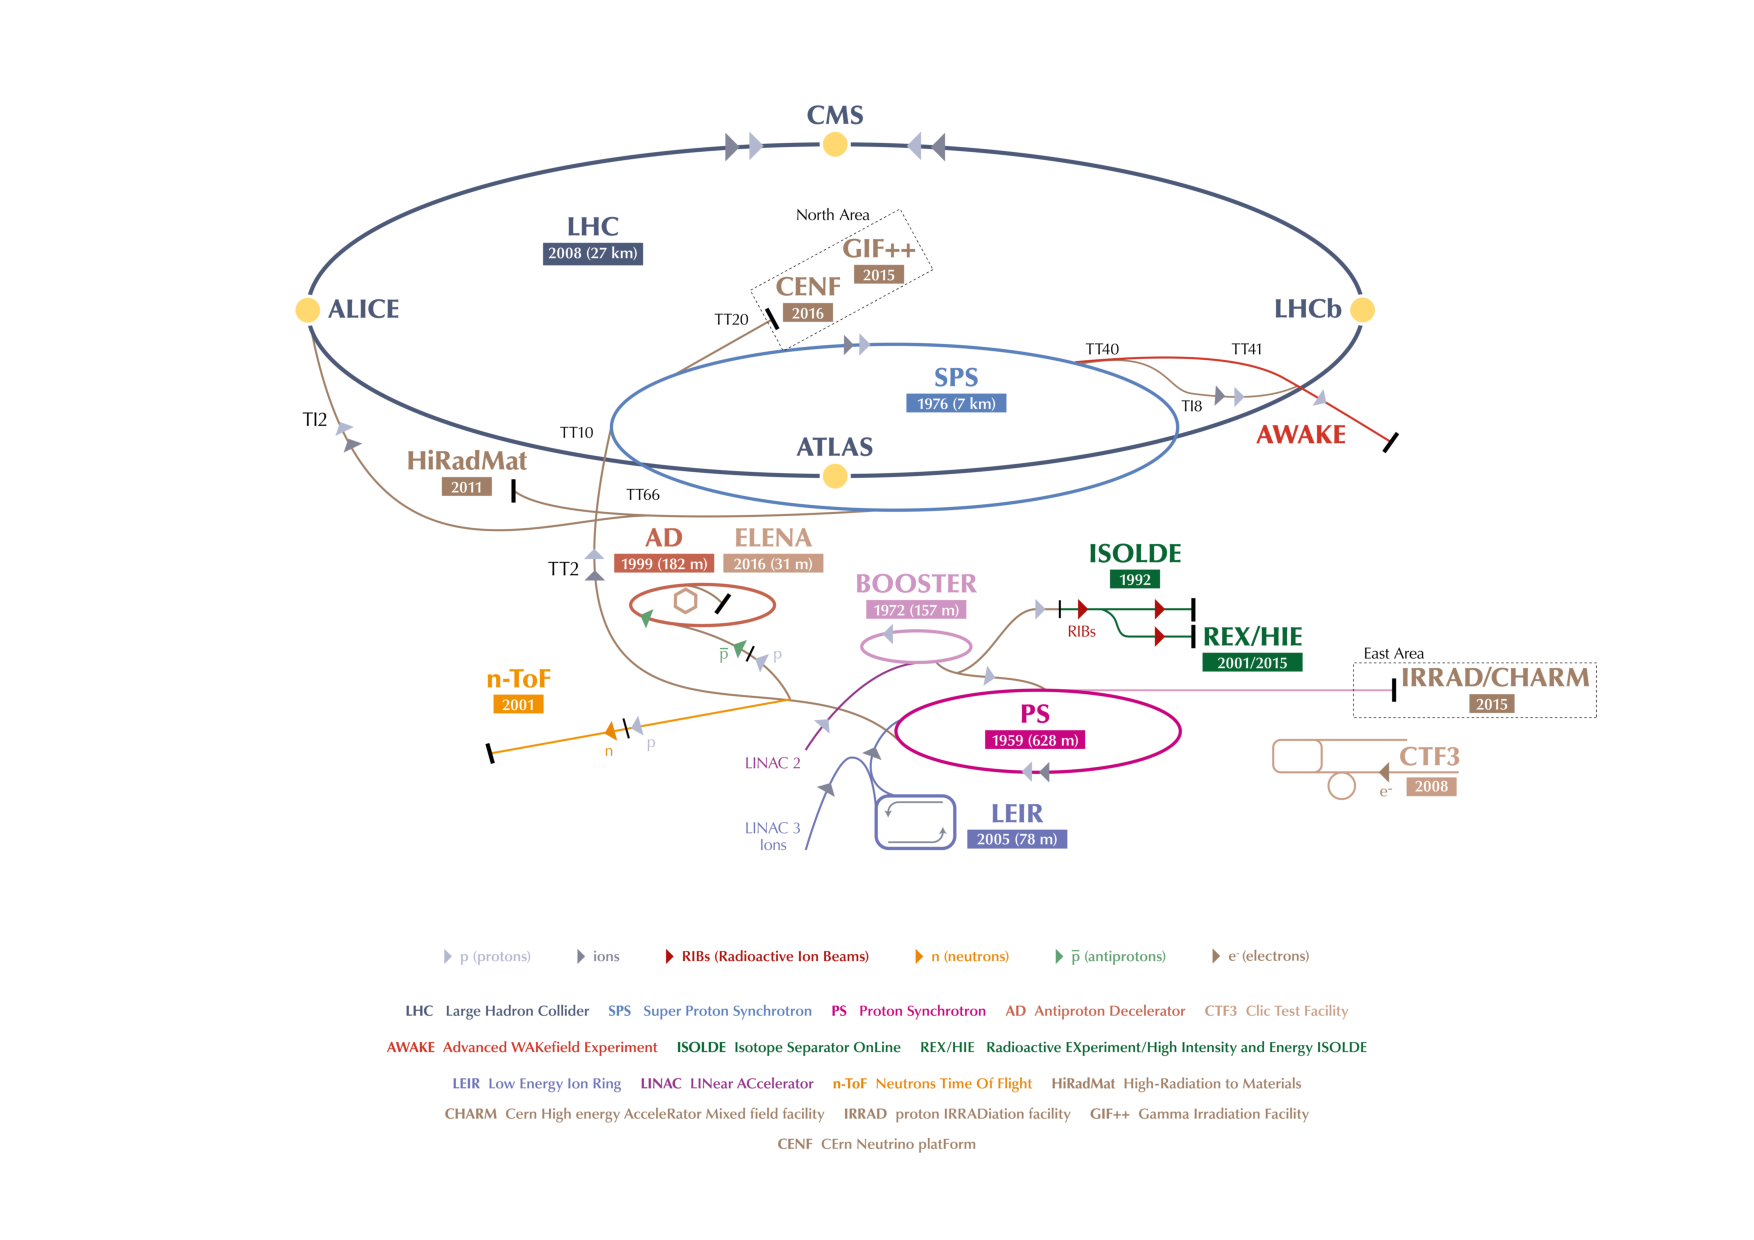
\includegraphics[width=1.15\textwidth,height=19cm]{figures/LHC/CERN_Accelerator_Complex-v2016.jpg}
	\caption{LHC accelerator chain along with all its other experiments which uses proton beam from other parts of accelerator either from PSB, PS or SPS\cite{Fig-CERN-accelerator-complex}}
	\label{fig:CERN-accelerator-complex}
\end{figure}
%%%%%%%%%%%%%%%%%%%%%%%%%%%%%%%%%%%%%%%%%%%%%%%%%%%%%%%%%%%%%%%%%%
%%%%%%%%%%%%%%%%%%%%%%%%%%%%%%%%%%%%%%%%%%%%%%%%%%%%%%%%%%%%%%%%%%
\subsection{Magnet System}
As the LHC is a circular collider; magnet system is one of the core parts and gives particles a circular trajectory in the LHC beam pipes. To be economical LHC has been made in eight arcs and eight straight sections instead of a perfect circle. Apart from bending the beam, it is also necessary to focus the two proton beams this is accomplished using a pair of quadrupole magnets, where the first magnet focus the magnet while other focuses the beam height as shown in Figure~\ref{fig:QuadrupoleMagnet}. A total of 858 quadrupole magnets are installed in LHC to keep the beams focused. Sextuple magnets are also used for proper focusing as every proton in the beam is not exactly with the same energy and on the same path. Several other magnetic multi-poles are used to keep the beam focused  in case the beam suffers from gravitational interactions over protons, electromagnetic interactions among bunches, electron clouds from pipe wall, and so on. Different types of magnets used in LHC are listed here \cite{WebLink:LHC_magnets}. Besides, there are eight sets of ``inner triplets" used at the four interaction points (IPs) to focus the beams during the collisions, to increase the luminosity. The size of bunch goes from 0.2 mm to 17 $\mu m$ at the interaction point of ATLAS or CMS. At the interaction point of ALICE or LHCb it is 71 $\mu m$. Summary of important parameters of LHC is given in Table~\ref{table:LHC-parameters}.
\begin{figure}[!htbp]
	\centering
	\includegraphics[width=0.65\textwidth]{figures/LHC/quadrupole_magnet_pair.png}
	\caption{Pair of quadrupole magnets.}
	\label{fig:QuadrupoleMagnet}
\end{figure}
% \begin{figure}[!htbp]
% 	\centering
% 	\includegraphics[width=0.95\textwidth]{figures/LHC/sextupole-octupole.jpg}
% 	\caption{Sextupole and octupole}
% 	\label{fig:sextupole-octupole}
% \end{figure}



\begin{table}
\vspace{-5.2em}
\centering
\begin{tabular}[!htbp]{l c}
\hline
{\bf Parameters} & {\bf Value} \\
\hline
Circumference of LHC ring   &   26658.883 m \\
\hline
Maximum dipole magnetic field   & 8.33 T \\
Dipole operating temperature    & 1.9 K \\
\hline
Maximum stored energy per beam (nominal) &   362 MJ \\
Maximum stored energy per beam  (2012) &   143 MJ \\
Maximum stored energy per beam  (2016) &   266 MJ \\
\hline
Beam energy at Injection    & 450 GeV \\
Beam energy at collision (nominal) &    7 TeV \\
Beam energy at collision (2012)     &   4 TeV \\
Beam energy at collision (2016)     &   6.5 TeV \\
\hline
Maximum instantaneous luminosity (nominal)  &   $10^{34}$ cm$^-2$ s$^{-1}$ \\
Maximum instantaneous luminosity (2012)     &   $7.7 \times 10^{33}$ cm$^-2$ s$^{-1}$ \\
Maximum instantaneous luminosity (2016)     &   $1.4 \times 10^{34}$ cm$^-2$ s$^{-1}$ \\
\hline
Number of bunches per proton beam (nominal) &   2808 \\
Number of bunches per proton beam (2012)    &   1380 \\
Number of bunches per proton beam (2016)    &   2076 \\
Maximum number of protons per bunch         &   $1.6 \times 10^{11}$ \\
\hline
Protons/bunch (average at start of collision) (nominal)   &   $1.15 \times 10^{11}$ \\
Protons/bunch (average at start of collision) (2012)  &   $1.5 \times 10^{11}$ \\
Protons/bunch (average at start of collision) (2016)  &   $1.1 \times 10^{11}$ \\
\hline
Bunch collision frequency (nominal)         &   40 MHz  \\
Bunch collision frequency (2012)            &   20 MHz  \\
Bunch collision frequency (2016)            &   40 MHz  \\
\hline
Bunch length (at injection)   &   1.7 ns \\
Bunch length (at collision)   &   1.05 ns \\
Energy spread (at injection)   &   1.9$\times 10^{-3}$ \\
Energy spread (at collision)   &   0.45$\times 10^{-3}$  \\
\hline
Half crossing angle  (nominal)   & 143 $\mu rad$ \\
Half crossing angle  (2012)   & 146 $\mu rad$ \\
Half crossing angle  (2016)   & 185 $\mu rad$ \\
\hline
$\beta *$  (nominal) &   0.55 m\\
$\beta *$   (2012)&   0.6 m\\
$\beta *$   (2016)&   0.4 m\\
\hline
RMS beam size at IP1 \& IP5 &   17 $\mu m$ \\
RMS beam size at IP2 \& IP8 &   71 $\mu m$ \\
\hline
$\epsilon_n$(transverse emittance, RMS, normalized) (at injection) &   3.5 $\mu$m\\
$\epsilon_n$(transverse emittance, RMS, normalized) (at collision point) &   3.75 $\mu$m\\
\hline
total longitudinal emittance (at injection) & 1.0 eVs \\
total longitudinal emittance (at collision) & 2.5 eVs \\
\hline
Average mean pile-up (nominal) &   25 \\
Average mean pile-up (2012) &    21 \\
Average mean pile-up (2016) &    27 \\
\hline
Energy loss per turn at 14 TeV              &   7 keV   \\
Energy loss per turn for electrons at 104.6 GeV          &  40,000 keV     \\
% synchtron radiation for electrons: Reference: Particle Physics Experiments at high energy colliders by John Hauptman
\end{tabular}
\caption{LHC technical parameters for proton-proton collisions: nominal, 2012 and 2016 values.\cite{Bruce2016, Schoerner-Sadenius2015, LHC-parameters-2016, LHC-tdr-vol1, cms-lumi-public-results}.}
\label{table:LHC-parameters}
\end{table}

%%%%%%%%%%%%%%%%%%%%%%%%%%%%%%%%%%%%%%%%%%%%%%%%%%%%%%%%%%%%%%%%%%
%%%%%%%%%%%%%%%%%%%%%%%%%%%%%%%%%%%%%%%%%%%%%%%%%%%%%%%%%%%%%%%%%%
\subsection{Key requirements of a particle accelerator} % (fold)
\label{sub:few_key_requirements}

The HEP collider is characterised based on two parameters centre of mass energy and the luminosity. The production rate of heavier particles like Higgs increases with the centre of mass energy. The luminosity is proportional to the number of events per second so it should be maximised. Luminosity is defined as:
\begin{equation}
    L = \frac{k_bN_b^2f_{rev}\gamma}{4 \pi \epsilon_n \beta^*}
\end{equation}
Where,\\
\hspace{2 cm}$k_b$ is the number of bunches per ring,\\
\hspace{2 cm}$N_b$ is the number of protons per bunch,\\
\hspace{2 cm}$f_{rev}$ the revolution frequency,\\
\hspace{2 cm}$\epsilon_n$ is the normalised RMS transverse beam emittance (same in both )\\
\hspace{2 cm}$\beta^*$ is the beta-function at the interaction point\\

Based on the definition of luminosity, we can maximise it by following ways:
\begin{itemize}
    \item By decreasing beam emittance, $\epsilon_n$.
    \item By improving the cryogenic system: As the factor $k_b.N_b$ is limited by thermal energy produced by synchrotron radiation.
    \item By decreasing beam-beam effect~\cite{Herr2014,Papotti2014}. As it scales with $N_b/ \epsilon_n$ which causes the spread in betatron tunes~\cite{Dubouchet2013}.
    \item Also, the space charge~\cite{Oeftiger2016} scales with $N_b/ \epsilon_n$.
\end{itemize}
% subsection few_key_requirements (end)

% section the_large_hadron_collider (end)

%%%%%%%%%%%%%%%%%%%%%%%%%%%%%%%%%%%%%%%%%%%%%%%%%%%%%%%%%%%%%%%%%%
\section{Experiments at the LHC} % (fold)
\label{sec:experiments_at_the_lhc}

At the LHC there are four IPs where the two proton beams are made to collide. At every IP one detector is placed. They are ATLAS, CMS, ALICE, and LHCb as shown in Figure~\ref{fig:LHCgeometry}. Also, there are two more small detectors LHCf and TOTEM installed close to the IP of the two main detectors ATLAS and CMS respectively.
\begin{figure}[!htbp]
	\centering
	\includegraphics[width=0.81\textwidth]{figures/LHC/lhc-schematic.jpg}
	\caption{LHC geometry with arcs and straight sections.}
	\label{fig:LHCgeometry}
\end{figure}
\newline
{\bf ATLAS} (A Toroidal LHC Apparatus) and {\bf CMS} (Compact Muon Solenoid) are the two large general-purpose\footnote{Here, general purpose means this machines will be used for many different kind of physics searches.} detectors having similar design and goal. CMS detector have been described in detail in Section~\ref{sec:cms_experiment}. The main difference in the two is in their magnet systems. This is motivated by the momentum resolution of muons. The momentum resolution for muons, $\Delta p_T/p_T$, is proportional to  $B^{-1}L^{-2}$, where B is magnetic field and L is the lever arm defined as the distance of momentum measurement from the IP of detector. So, to improve the momentum resolution there are two possible choices.

\begin{enumerate}
	\item Increase the magnetic field with compact design, or
	\item Work with low magnetic field with long lever arm
\end{enumerate}

There is also a third possibility to improve the momentum resolution by increasing the leaver arm as well as magnetic field, but it increases the cost of the detector by several factors. So, CMS chooses the first point, i.e., to increase the magnetic field with compact design\footnote{This is why there is word {\bf compact} in the name of CMS.} while ATLAS chooses the design with low magnetic field with long lever arm.

% ATLAS has an eight toroidal magnets combined with a smaller inner solenoid while CMS has a powerful solenoid magnet only.

{\bf ALICE} (A Large Ion Collider Experiment) is a heavy-ion detector. It is specially designed for the study of strongly interacting matter at high densities in quark-gluon plasma phase.

{\bf LHCb} (Large Hadron Collider beauty) is made asymmetrically with respect to the IP of the detector. It is designed specially to investigate the matter-antimatter asymmetry through the study of b-quarks.

{\bf LHCf} (Large Hadron Collider forward) and {\bf TOTEM} (TOTal cross-section, Elastic scattering and diffraction dissociation Measurement at the LHC) are there for the study of forward physics\todo[fancyline]{define forward physics}.
% section experiments_at_the_lhc (end)

% %%%%%%%%%%%%%%%%%%%%%%%%%%%%%%%%%%%%%%%%%%%%%%%%%%%%%%%%%%%%%%%%%%
\section{CMS Detector} % (fold)
\label{sec:cms_experiment}
The design and components of a HEP detector depends upon the physics goals and operation parameters of the particle accelerator. In case of the CMS detector, following challenges are imposed from the LHC:
\begin{itemize}
	\item \textbf{High luminosity:} A high value of  delivered luminosity that implies every-time the two proton bunches cross each other there will be more than one p-p interactions\footnote{More than one p-p interaction in one bunch crossing is known as pile-up. It can be theoretically estimated as the product of inelastic p-p cross-section ($\sigma_{inel}$), instantaneous luminosity ($L$) and the mean time interval between two collision, ($< t >$). \begin{equation}
		mean~pile-up = \sigma_{inel} \times L \times <t>
	\end{equation}}. Given this, there will be more than $\mathcal{O}(1000)$ particles passing through detector during every p-p collision. Thus, the detector should be highly granular which results in increased number of readout channels that should be synchronised with LHC clock.
	\item \textbf{Response time:} At LHC, the two proton beams cross each other every 25 ns. So, the response time of all the sub-detector systems should be less than 25 ns.
	\item \textbf{Radiation hardness:} At every 25 ns the detectors are bombarded with more than 1000 particles so all the sub-detectors should be radiation hard including its electronics, cables, glue, screws, and so on.
\end{itemize}

Restrictions imposed on detector from the physics goals of the LHC:

\begin{itemize}
	\item Good muon identification and momentum resolution ($\approx$ 1\% at 100 GeV).
	\item Efficient triggering and tracking of b-jets and $\tau$'s.
	\item Highly efficient and granular electromagnetic calorimeter to detect and measure energies of electrons and photons.
	\item Good missing transverse energy resolution and di-jet mass resolution requires a ``hermetic'' hadron calorimeter with full geometric coverage and fine lateral segmentation.
\end{itemize}

% When the two beam of proton collides then thousands of particles are produced and out of them only 9 particles are of interest from detector construction point of view. They are photons ($\gamma$), electrons ($e$), muons ($\mu$), pions ($\pi^{\pm}$), kaon ($K^{\pm},~K_L,~K_S$), protons ($p$), and neutrons ($n$). Out of rest there are three neutrinos which interacts only weakly that do not interact in light mass HEP detectors and others are short lived particles. So, 

Based on the above conditions CMS detector is designed in a cylindrical shape having each detector on top of the other with beam pipe at the centre. To have a full geometric coverage, it is designed with a barrel region and two endcap regions. Main part of the CMS detector is its superconducting magnet system, capable of producing a highly uniform magnetic field of 4T to accurately measure the high momentum particles, while the muon detector system are kept outside the magnet but sandwiched in its return yoke. While the tracking system and calorimeters are placed inside the magnet. CMS detector design is shown in Figure~\ref{fig:CMS-detector}.
\begin{figure}[!htbp]
	\centering
	\includegraphics[width=0.95\textwidth]{figures/LHC/cms_120918_03.png}
	\caption{CMS detector drawing}
	\label{fig:CMS-detector}
\end{figure}

\subsection{Coordinate System} % (fold)
\label{sub:coordinate_system}
Right handed coordinate system is used at the CMS detector, having origin at the nominal IP (Figure~\ref{fig:cms-coordinate-system}). Z-axis is considered along the beam direction in such a way so that x-axis will point radially to the centre of LHC ring and y-direction is pointing upwards. The azimuthal angle, $\phi$, is measured in the x-y plane from x-axis and the polar angle, $\theta$, is measured from the z-axis. Instead of describing a particle at some polar angle we prefer to use the variable pseudo-rapidity. It is defined as 
\begin{equation}
	\eta = -ln\bigg[tan\Big(\frac{\theta}{2}\Big)\bigg]
\end{equation}
In the hadron collider use of pseudo-rapidity was motivated from the invariance of its difference, $\Delta \eta$, with respect to the particle boost direction. Also, the particle density remains constant in barrel region of the detector, measured in equal rapidity intervals.

\begin{figure}[htbp]
	\centering
	\includegraphics[width=0.95\textwidth]{figures/LHC/CMS-coordinate-system.png}
	\caption{Right handed coordinate system used by CMS.}
	\label{fig:cms-coordinate-system}
\end{figure}

% subsection coordinate_system (end)
%%%%%%%%%%%%%%%%%%%%%%%%%%%%%%%%%%%%%%%%%%%%%%%%%%%%%%%%%%%%%%%%%%
%%%%%%%%%%%%%%%%%%%%%%%%%%%%%%%%%%%%%%%%%%%%%%%%%%%%%%%%%%%%%%%%%%
\subsection{CMS sub-systems} % (fold)
\label{sub:cms_sub_systems}

%%%%%%%%%%%%%%%%%%%%%%%%%%%%%%%%%%%%%%%%%%%%%%%%%%%%%%%%%%%%%%%%%%
%%%%%%%%%%%%%%%%%%%%%%%%%%%%%%%%%%%%%%%%%%%%%%%%%%%%%%%%%%%%%%%%%%
\subsubsection{Magnet} % (fold)
\label{ssub:magnet}
Magnet system of CMS consists of a superconducting solenoid magnet which is 12.5 m in length and has an inner diameter of 6m. The size of solenoid is large as the tracker, electromagnetic calorimeter and hadron calorimeter are placed inside the solenoid. In barrel region it generates homogeneous magnetic field of 3.8 T. The high magnetic field ensures the appropriate bending power for the highly energetic charged particles to precisely measure their momentum. Outside the solenoid iron yoke is placed for the returning magnetic field. The magnetic field strenght inside the iron yoke is 2 T. Figure~\ref{fig:CMS-magnet} shows the CMS magnet.

\begin{figure}[!htbp]
	\centering
	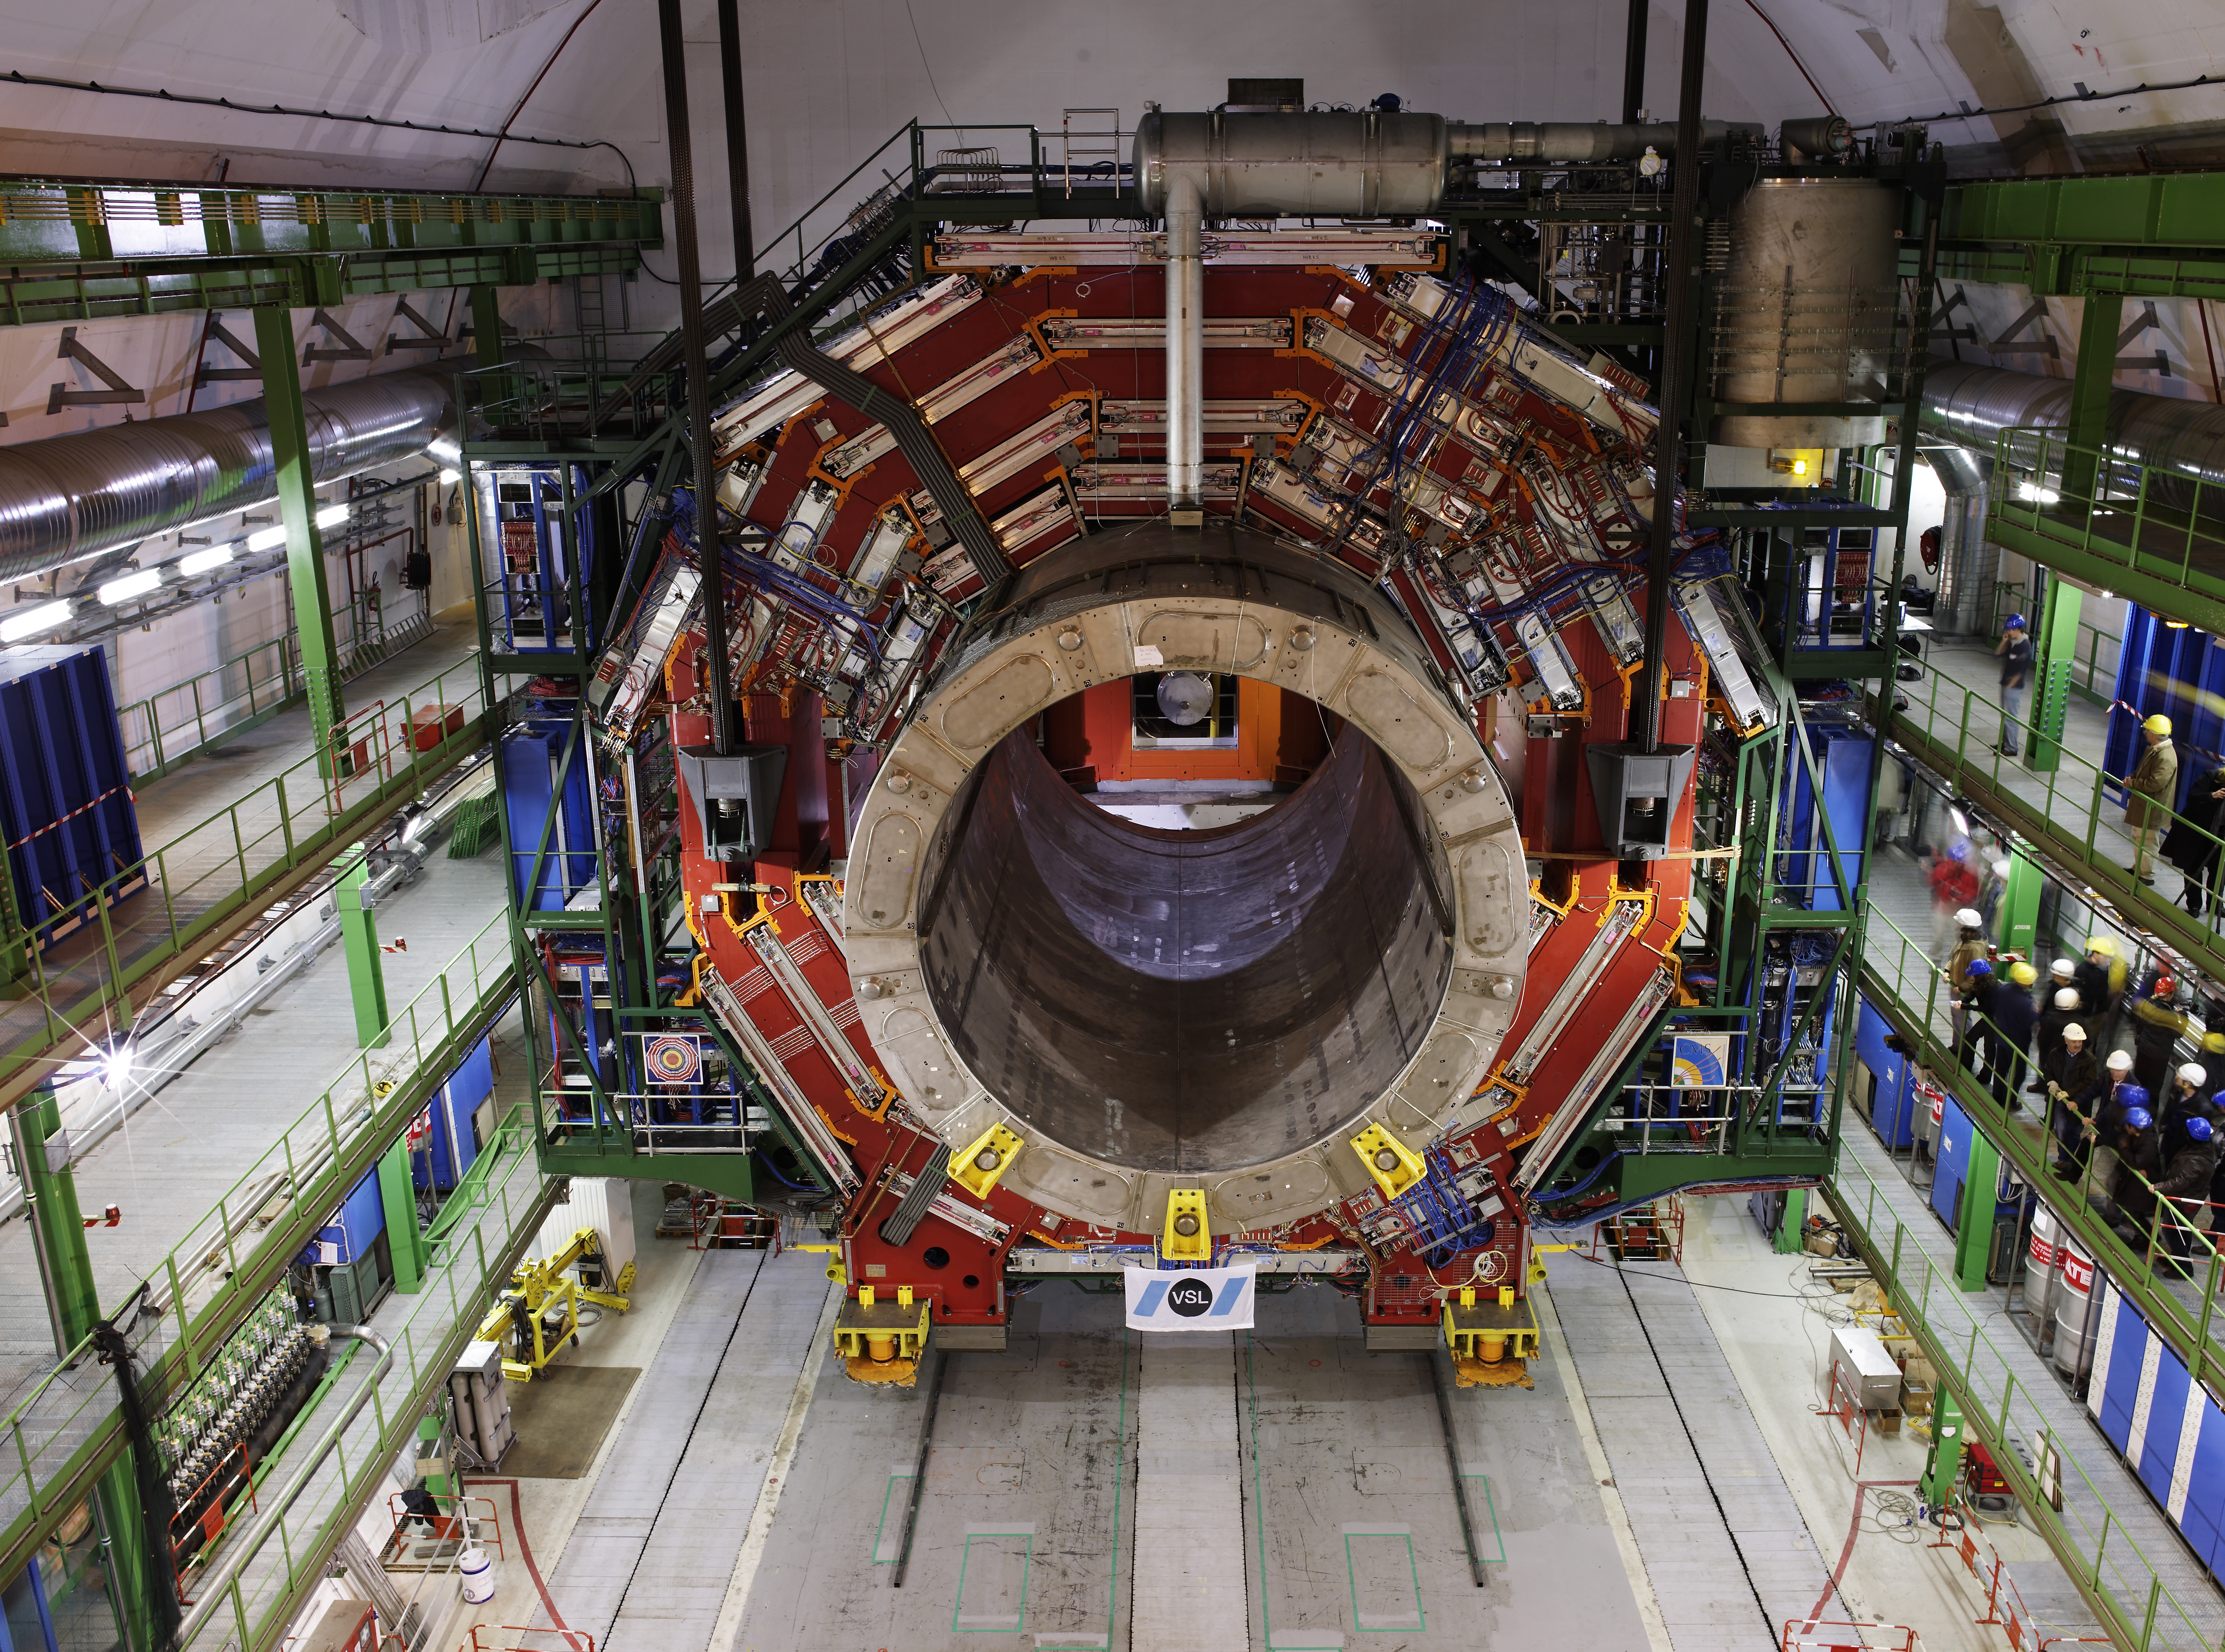
\includegraphics[width=0.95\textwidth]{figures/LHC/CMS_magnet.jpg}
	\caption{CMS Magnet system}
	\label{fig:CMS-magnet}
\end{figure}

% subsubsection magnet (end)
%%%%%%%%%%%%%%%%%%%%%%%%%%%%%%%%%%%%%%%%%%%%%%%%%%%%%%%%%%%%%%%%%%
%%%%%%%%%%%%%%%%%%%%%%%%%%%%%%%%%%%%%%%%%%%%%%%%%%%%%%%%%%%%%%%%%%
\subsubsection{Tracker} % (fold)
\label{ssub:tracker}
Tracker is the first detector that encounters the particles emerging from the p-p collisions. Its purpose is to measure precisely the tracks of all charged particles crossing it. Also, it helps to reconstruct the secondary vertices to tag heavy flavour particles like b-jets or tau leptons. The particle rate is highest in the tracker. So, it should be highly granular and response time should be fast. This condition results in high density of on-detector electronics and this implies a large amount of materials that conflicts with the aim of low material to reduce the multiple scattering, bremsstrahlung, photon conversion and nuclear interactions. Thus, the type, design and number of layers of tracker is the trade-off between the performance, the amount of material, and the cost. Considering these things in mind CMS collaboration decided to have first three layers of silicon pixel detector to precisely measure the primary vertex, secondary vertex and the impact parameter with a total surface area of 1 $m^2$ and 66 million pixels followed by 10 layers of  silicon micro-strip detector covering a total area of 200 $m^2$. Tracker has length of 5.8 m and outer diameter 2.6 m and acceptance is up to $|\eta|<2.5$. Tracker's cross sectional view is shown in Figure~\ref{fig:tracker-cross-section}.

\begin{figure}[!htbp]
	\centering
	\includegraphics[width=0.95\textwidth]{figures/LHC/tracker-cross-section.png}
	\caption{Systematic cross section view of CMS tracker showing silicon pixel and strip detectors. Double line shows back-to-back modules that delivers stereo hits.}
	\label{fig:tracker-cross-section}
\end{figure}
% subsection tracker (end)

%%%%%%%%%%%%%%%%%%%%%%%%%%%%%%%%%%%%%%%%%%%%%%%%%%%%%%%%%%%%%%%%%%
%%%%%%%%%%%%%%%%%%%%%%%%%%%%%%%%%%%%%%%%%%%%%%%%%%%%%%%%%%%%%%%%%%

\subsubsection{Calorimetry} % (fold)
\label{ssub:calorimetry}
In general, the calorimeter is a device that measures the energy of particles by absorbing. The CMS detector uses two different type of calorimeter based on their interaction. They are Electromagnetic CALorimeter (ECAL) and Hadronic CALorimeter (HCAL). ECAL as the name suggest it is designed to measures the particles (electrons and photons) that primly interact via electromagnetic interaction while HCAL is designed to measure particles that interact via strong nuclear interactions.\\\\
ECAL is placed after tracker for the detection of  electrons and photons. It is a homogeneous calorimeter made from lead tungstate ($PbWO_4$) crystals, having a coverage up-to $\eta < 3.0$ including pre-shower system in forward region. The scintillation produced in barrel region is detected by Avalanche photo-diodes and in endcaps it is collected by vacuum photo-triodes. In terms of radiation length\footnote{Radiation length is defined as the mean length travelled by particle to reduce its energy by the factor of 1/e.}, $X_0$, its thickness is 25$X_0$ which guarantees almost full shower containment.\\\\
In between ECAL and magnet system, brass/scintillator sampling HCAL with coverage up to $\eta < 3.0$ is placed. To have a full geometric coverage HCAL is extended up to $\eta < 5.0$ using forward sampling iron/quartz-fibre calorimeter. This is crucial to measure the (missing) transverse energy of the event.

% The energy resolution of the ECAL can be parameterized  
% subsubsection calorimetry (end)


%%%%%%%%%%%%%%%%%%%%%%%%%%%%%%%%%%%%%%%%%%%%%%%%%%%%%%%%%%%%%%%%%%
%%%%%%%%%%%%%%%%%%%%%%%%%%%%%%%%%%%%%%%%%%%%%%%%%%%%%%%%%%%%%%%%%%
\subsubsection{The Muon System} % (fold)
\label{sub:the_muon_system}
From the name of CMS detector it is evident that the precise detection of muons is one of its main target. It is motivated by the presence of muons in the final state of many interesting physics processes, such as, the decay of Higgs boson into ZZ which subsequently decay in four leptons and especially, the case where all 4 leptons are muons is refereed to as the ``gold plated'' channel as we can detect muons efficiently over higher background contributions at LHC. At CMS, muon system serves three different functions viz. identification, momentum measurement and triggering of muons. The strong superconducting magnet system with its return yoke of CMS, helps to acquire good momentum measurement and triggering capabilities. The return yoke of magnet system also serves as the hadron absorber. Only muons leave their tracks in the muon detector system, as all other particles are already absorbed by the calorimeters. Thus, the appearance of charged particle in the muon system signifies that it can only be muons. The track left by muon in the CMS detector is illustrated in Figure~\ref{fig:muon-system-cross}. 
\begin{figure}[!htbp]
	\centering
	\includegraphics[width=0.55\textwidth]{figures/LHC/MuStations.png}
	\caption{A muon leaves curved trajectory in LHC and the bending changes as the magnetic field direction of solenoid inside and outside are opposite.}
	\label{fig:muon-system-cross}
\end{figure}
The layout of the CMS muon detector system is shown in Figure~\ref{fig:muon-system-layout}. Three different types of gaseous detectors used for the muon system which were chosen based on the background level, muon rate, uniformity and magnitude of magnetic field. Drift tubes are used as tracking detector in the barrel region with relatively lower magnetic field intensity and which have lower background rates as compared to the endcaps. 
For the endcap regions Cathode Strip Chamber (CSC) are employed as they are provide precise information about muons momentum and time information even in high radiation environment. The pseudo-rapidity coverage of DTs is $|\eta|<1.2$ and for CSCs is $0.9<|\eta|<2.4$. Along with DTs and CSCs, Resistive Plate Chamber (RPC) detectors are also installed to have a fast dedicated  muon triggering system in both barrel and endcap region up to $|\eta|<1.6$~\cite{muon-tdr}. The CMS muon detector system covers the geometric region up-to $|\eta|<2.4$ but RPCs are deployed up-to $|\eta|<1.6$ as RPCs cannot withstand the radiation level after pseudo-rapidity region of 1.6. Thus to reconstruct muons in pseudo-rapidity region higher than 1.6, CMS collaboration decided to employ Gas Electron Multiplier (GEM) detectors in region  $1.6<|\eta|<2.2$, which is able to provide good space resolution and time resolution even in high environment radiation during Long Shutdown-2 (LS2, 2019-2020). The pseudo-rapidity range is limited to $|\eta|<2.2$ because of space constrains. GEM  detectors are described in details in Chapter~\ref{ch:gem}.
\begin{figure}[!htbp]
	\vspace{-3.2em}
	\centering
	\includegraphics[width=0.85\textwidth]{figures/LHC/pictures_MuonSys-mod3.png}
	\caption{Longitudinal layout of one quadrant of the CMS detector. There are four DT stations named MB1-MB4 marked with green colour. Four CMS system in high pseudo-rapidity region named ME1-ME4 in blue colour. Also, there are several RPC stations in barrel region and part of endcap region marked with red colour.}
	\label{fig:muon-system-layout}
\end{figure}
Summary of CMS detector sub-system including its main characteristics and composition is given in Table~\ref{table:CMSMainChar}.
% subsection the_muon_system (end)
% subsection cms_sub_systems (end)
% % section cms_experiment (end)

\begin{table}
% \vspace{-5.2em}
\centering
\begin{tabular}[!htbp]{l l l}
\hline
{\bf Sub-system} & {\bf Composition} & {\bf Charateristics} \\
\hline
Tracker  & silicon strip and  & isolated track effiency $\epsilon > 95\%$ \\
	& pixel detector	& within jets $\epsilon \sim 90\%$ \\
	& 	& primary vertex resolution: 10-20 $\mu m$ \\
	& 	& $p_T$ resolution: $\Delta p_T/p_T = 1\%$ (0.1 TeV), 10\% (TeV)\\
	& 	& coverage $\eta<2.5$ \\
\hline
ECAL 	& 	$PbWO_4$ crystals 	& energy resolution:\\
		& 	& $\big(\frac{\sigma}{E}\big)^2 = \big(\frac{2.7\%}{\sqrt{E}}\big)^2 + \big(\frac{210}{E}\big)^2 + 0.55\% $  (barrel)\\
		& 	& $\big(\frac{\sigma}{E}\big)^2 = \big(\frac{5.7\%}{\sqrt{E}}\big)^2 + \big(\frac{245}{E}\big)^2 + 0.55\% $  (end-caps)\\
		& 	& coverage $\eta < 3$ \\
\hline
HCAL 	& 	Cu-Zn 	& energy resolution:\\
		& 	scintillators & $\big(\frac{\sigma}{E}\big)^2 = \big(\frac{68\%}{\sqrt{E}}\big)^2 + 4.5\%$ \\
		& 	& coverage $\eta < 3$ \\
\hline
Muon system & gaseous & efficiency $\epsilon \sim 98\%$ \\
			& detectors & $\Delta p_T/p_T =$8-15 \% (0.01 TeV)/20-40\% (TeV)\\
		& 	& coverage $\eta < 2.4$ \\
\hline
\end{tabular}
\caption{Main characteristics of the CMS sub-system~\cite{JeremieThesis}}
\label{table:CMSMainChar}
\end{table}


% %%%%%%%%%%%%%%%%%%%%%%%%%%%%%%%%%%%%%%%%%%%%%%%%%%%%%%%%%%%%%%%%%%
\subsection{CMS Trigger and Data Acquisition system} % (fold)
\label{sub:cms_trigger_and_data_acquisition_system}
The LHC produces 1 billion p-p collisions every second and thousands of particles produced during these collisions cross the CMS detector and reconstruction of these events generates several Terabytes of data. However, till now we neither have a switch with the required bandwidth that can transfer enormous data for further processing nor the disk space to store all of them. Even if we have one, then there are only a few fractions of data that are interesting for new physics or help to understand the existing one as most of the collisions is the low-energy glancing collision instead of head-on interaction. The maximum amount of data that can be stored every day is of the order of few Terabytes that decides the rate at which we can accept the events ($\sim$ 100 Hz).The concept of the trigger, method to select events of interest, was first introduced by ZEUS experiment~\cite{ZEUSCollaboration1993}, that handles data in real time, coupled with complex data acquisition system. While designing the trigger one has to keep in mind that trigger should efficiently accept the interesting physics while rejecting the non-interesting ones as whatever information lost at this level can not be recovered.

The CMS trigger system is divided into two steps, level 1 (L1) trigger which is a custom hardware process running synchronously with the LHC bunch crossing frequency of 40 MHz and the High-Level Trigger (HLT)~\cite{paper:JINST:CMSCollaboration}. The L1 trigger system analyses the events based on the information of calorimeter and muon system and  then selects the interesting events. However, this decision cannot take place within 25 ns, so a latency of 3.2 $\mu s$ was added. The maximum allowed frequency at the L1 stage is 100 kHz. Then the complete information is sent to HLT processing farm to reduced the event rate to $\sim$100 Hz. The remaining information is sent to Tier-0 centres to store and use it for offline analysis.



% section cms_trigger_and_data_acquisition_system (end)

% %%%%%%%%%%%%%%%%%%%%%%%%%%%%%%%%%%%%%%%%%%%%%%%%%%%%%%%%%%%%%%%%%%
\subsection{CMS Offline Computing} % (fold)
\label{sub:cms_offline_computing}
Once the data are selected by the trigger system, they are ready to be analysed offline. Before that, the raw data need to be processed, i.e., to convert data into understandable physics objects like electrons, muons, photons, jets, and so on. This step is known as object reconstruction which is the most CPU intensive task in the data processing chain of CMS. In this step one needs to reconstruct the primary vertices, charged particle tracks, identify electrons, photons, muons, reconstruct jets, apply b-tagging algorithm to reconstruct b-jets, run detector specific filtering and so on.
To perform all these steps CMS developed its software which is known as CMSSW. This software is based on Event Data Model (EDM) centred around the concept of the event. Here, an event is a C++ object container for all raw and reconstructed data related to a particular collision. Finally, these events are stored in ROOT files~\cite{Root1996}. The CMSSW event processing model consists of one executable called cmsRun, and many plug-in modules. These modules contain all the necessary codes for the event processing such as calibration and reconstruction algorithms~\cite{Bayatyan2005}.
To analyse data, we also need MC simulations which are carried out based on the predictions of SM and various new physics models. MC events are generated at parton level. Then showering and hadronization is applied, and finally, these events are put through the GEANT4~\cite{Agostinelli2003} based CMS detector simulation. The result is data similar to what one obtains from the actual detector. This MC data can then also be reconstructed as if it were  detector data.


% section cms_offline_computing (end)




% \begin{figure}[!htbp]
% 	\centering
% 	\includegraphics[width=0.95\textwidth]{figures/lumi-proj-2016-final-v2}
% 	\caption{The integrated luminosity of the LHC with proton-proton collisions in 2016 compared to previous years. Luminosity is a measure of a collider’s efficiency and is proportional to the number of collisions. The integrated luminosity achieved by the LHC in 2016 far surpassed expectations and is double that achieved at a lower energy in 2012. (Image : CERN)\todo[inline]{Update the caption.}}
% 	\label{fig:lumi-proj-2016-final-v2}
% \end{figure}





% Because of limited geometrical space in LHC ring the beam pipe was designed as a ``twin-aperture" magnets, where superconducing ring is housed in a common return yoke and cryostat.

% chapter the_lhc_and_cms_machine (end)


% \begin{figure}[!htbp]
% 	\centering
% 	\includegraphics[width=0.95\textwidth]{figures/LHC/cms_complete_labelled.png}
% 	\caption{CMS detector drawing}
% 	\label{fig:CMS-detector-2}
% \end{figure}

  % \chapter{Gas Electron Multiplier} % (fold)
\label{cha:gas_electron_multiplier}

\section{Introduction} % (fold)
\label{sec:introduction}

% section introduction (end)
The invention of Multi-Wire Proportional Chamber (MWPC) in 1968 by Georges Charpak was one of breakthrough in gaseous detectors, since it had better rate capability vis-a-vis its predecessors~\cite{Charpak1968}. 
This invention was also led to Nobel prize to George Charpak in 1992. With time the design and performance of MWPC have been improved. But because of our increasing demands with the acquired knowledge its limitation reached in terms of the maximum rate capability and granularity. In 1988 Anton Oed invented the Micro-Strip Gas Counter (MSGC). 
This detector had overcome the rate limitation due to positive-ion accumulation in the gas volume and able to reach up to few tens of micron in position resolution. 
Also, it can sustain the particle flux exceeding the $MHz/mm^2$ range. Its performance was very impressive but long-term study revealed its two weakness. They are:
\begin{enumerate}
	\item Formation of deposits on the electrodes, which affects the gain and age of the detector.
	\item In presence of highly ionizing particles sometimes a destructive discharge happens.
\end{enumerate}
The invention of Micro-Pattern Gaseous Detector (MPGD) focuses these issues. 
It has unprecedented spatial resolution, large sensitive area, high rate capability, operational stability along with long life-time in particular the Gas Electron Multiplier (GEM)~\cite{Sauli1997,Sauli1999} detectors. 
Several new study also shown that if a reasonable precaution are taken on the component quality it might be less vulnerable to the radiation induced ageing than the standard silicon micro-strip detectors~\cite{TITOV2004,Titov2002}.

% \section{GEM Introduction \& Operational Principle} % (fold)
% \label{sec:gem_introduction_&_operational_principle}
GEM is a new concept from Fabio Sauli at CERN \cite{Sauli1997}. It was introduced to improve the performance of microstrip gas chamber and to match the harsh running conditions of experiments at CERN's LHC collider, where detectors will have to cope with high data rates and will be exposed to intense bombardment by high-energy particles \cite{detector:1732870}.

It is a thin plastic sheet coated with metal on both sides and chemically pierced by a regular array of holes a fraction of a millimetre across and apart. 
Applying a voltage (about 500V on 50$\mu$) across the GEM conducting layers, the resulting high electric field in the holes makes an avalanche of ions and electrons pour through each. 
The GEM foil is shown in Figure \ref{fig:gem}.
\begin{figure}[!htbp]
	\centering
	\includegraphics[width=0.95\textwidth]{figures/GEM/KEKDTP3.jpg}
	\caption{(Left) The gas electron multiplier (GEM) foil can image two-dimensional position of particles passing through a gaseous chamber. (Right) The cross sectional view of the GEM shows strong electric fields in the vicinity of holes where electron signals are amplified.}
	\label{fig:gem}
\end{figure}
The region inside GEM detector have three different regions: drift electrode, a conversion and drift region.
%, a GEM mesh collecting and multiplying the charge in a gas avalanche, and induction gap in which a high electric field is used to extract and drift the electrons towards the collecting electrodes. This is shown in Figure \ref{fig:gemgaps}. 
The large effective gains (up to $10^4$), full efficiency of detection and very good localization accuracies for minimum ionizing particles is promising to us. 
In the thin gap of GEM few tens of primary ion pairs creates; cascading to two GEM meshes so it can provide large gains and better performances with very less probability of discharge~\cite{Bressan1999}.
\begin{figure}[!htbp]
	\begin{center}
		\includegraphics[width=0.95\textwidth]{figures/GEM/triple_gem.png}
		\caption{Illustration of GEM working}
		\label{fig:gemgaps}
	\end{center}
\end{figure} 
% section gem_introduction_&_operational_principle (end)
\section{Fabrication \& Characterization} % (fold)
\label{sec:fabrication_&_characterization}
\subsection{Foil Production}
Through Transfer of Technology (TOT) Micropack signed an agreement for the development of GEM foils in India in collaboration with Indian Institutions. 
After continuous efforts, refining of processes and repeated trials, Micropack has been successful in realizing $10~cm~\times~10~cm$ and $30~cm~\times~30~cm$ GEM foils, meeting the standard dimensional requirements.
Micropack started the production with single mask process as this configuration is the one we are going to use in CMS detector.
But, after several attempts they realized that this is quite challenging so they switched to double mask process. They quickly succeeded in production of the double-mask GEMs.
It is produced in a similar fashion as at CERN PCB workshop~\cite{DEOLIVEIRA2009}.
The foil used by Micropack was 50 $\mu m$ PI (Apical Type NP) film with 5 $\mu m$ copper coating on both side. Figure~\ref{fig:Foil_and_Cone}(a) shows the $10~cm~\times~10~cm$ GEM foil produced by Micropack and the Fig.~\ref{fig:Foil_and_Cone}(b) shows the cross-sectional view of the foil showing the double conical structure.
To qualify these GEM foils as commercially and scientifically reliable, a number of quality control test have to be performed. 
The two main quality control tests are optical test and electrical test. The optical test gives us information about the quality of produced foil like the hole geometry, pitch information and about the defects, if any. 
While the electrical test gives us information about the leakage current, discharge effects, etc.
\begin{figure}[!htbp]
    \centering
    \begin{subfigure}[b]{0.46\textwidth}
        \includegraphics[width=6cm, height=4cm]{figures/GEM/figures/Foil_01.png}\qquad
        \caption{ }
    \end{subfigure}
    \begin{subfigure}[b]{0.46\textwidth}
        \includegraphics[width=6cm, height=4cm]{figures/GEM/figures/double_cone.png}
        \caption{ }
    \end{subfigure}
   \caption{(a) 10 cm $\times$ 10 cm GEM foil encapsulated in a frame and (b) Cross-sectional view of the foil showing the double cone structure of the engraved holes. } \label{fig:Foil_and_Cone}
\end{figure}

\subsection{Optical Assessment}
GEM performance depends heavily on the quality and parameters of GEM foil like thickness of foil, hole diameter, pitch, and defects like missing holes, un-etched areas, excess-etching, burnt areas, etc. 
To check these defects and to measure the hole-size and pitch several method was developed using an automated 2D-CCD scanner~\cite{Posik2015, Becker2006}. 
However we used a different technique. We divided the GEM foil into several sectors and captured a high resolution picture using the AF-S Micro Nikon 40 mm 1:2.8G lens. We used a soft box ($1~m~\times~1~m$) light source for uniform illuminating the GEM foil.
A sketch of the set-up is shown in Fig.~\ref{fig:Optical_Sketch}.
\begin{figure}[!htbp]
    \centering
    %\begin{subfigure}[b]{0.7\textwidth}
        %\includegraphics[width=12cm, height=8cm]{figures/GEM/figures/NIMA_paper_Images001.jpeg}
        \includegraphics[width=12cm, height=8cm]{figures/GEM/figures/2.jpeg}
        %\includegraphics[width=9cm, height=8cm]{figures/GEM/figures/Optical_Sketch.png}
    %    \caption{ }
    %\end{subfigure}
   \caption{Sketch of the set-up used for the optical measurements.}   \label{fig:Optical_Sketch}
\end{figure}
Fig~\ref{fig:Optical_01} shows the found defects in the considered GEM foil. Also, the measured number of defects are shown in Fig.~\ref{fig:Optical_04}.
\begin{figure}[!htbp]
    \centering
    \begin{subfigure}[b]{0.29\textwidth}
        \includegraphics[width=4cm, height=3cm]{figures/GEM/figures/3a.jpg}
        \caption{ }
        \label{fig:O_4a}
    \end{subfigure}
    \begin{subfigure}[b]{0.29\textwidth}
        \includegraphics[width=4cm, height=3cm]{figures/GEM/figures/3b.jpg}
        \caption{ }
        \label{fig:O_4b}
    \end{subfigure}
    \centering
    \begin{subfigure}[b]{0.29\textwidth}
        \includegraphics[width=4cm, height=3cm]{figures/GEM/figures/3c.jpg}
        \caption{ }
        \label{fig:O_4c}
    \end{subfigure}
    \centering
    \begin{subfigure}[b]{0.29\textwidth}
        \includegraphics[width=4cm, height=3cm]{figures/GEM/figures/3d.jpg}
        \caption{ }
        \label{fig:O_5a}
    \end{subfigure}
    \centering
    \begin{subfigure}[b]{0.29\textwidth}
        \includegraphics[width=4cm, height=3cm]{figures/GEM/figures/3e.jpg}
        \caption{ }
        \label{fig:O_5b}
    \end{subfigure}
    \centering
    \begin{subfigure}[b]{0.29\textwidth}
        \includegraphics[width=4cm, height=3cm]{figures/GEM/figures/3f.jpg}
        \caption{ }
        \label{fig:O_5c}
    \end{subfigure}
   \caption{Observed imperfections in the foils: (a) Un-etched area, (b) under-size hole, (c) over-size hole (d) missing hole, (e) excess etching and (f) burnt area.} \label{fig:Optical_01}
\end{figure}

% as shown in the Figures \ref{fig:Optical_02} (a) and \ref{fig:Optical_02} (b), respectively. 
% \begin{figure}[!htbp]
%     \centering
%     \begin{subfigure}[b]{0.44\textwidth}
%         \includegraphics[width=5cm, height=4cm]{figures/GEM/figures/O_1b}
%         \caption{ }
%         \label{fig:O_1a}
%     \end{subfigure}
%     \begin{subfigure}[b]{0.44\textwidth}
%         \includegraphics[width=5cm, height=4cm]{figures/GEM/figures/O_1a}
%         \caption{ }
%         \label{fig:O_1b}
%     \end{subfigure}
%    \caption{(a) Outer holes when front light is ON and (b) Inner holes when back light is ON.} \label{fig:Optical_02}
% \end{figure}
%=====================================================================	
%=====================================================================

\begin{figure}[!htbp]
    \centering
    \begin{subfigure}[b]{0.49\textwidth}
        \includegraphics[width=7.6cm, height=5.5cm]{figures/GEM/figures/Apical_Defects.pdf}\qquad
        \caption{ }
        \label{fig:O_9a}
    \end{subfigure}
    \begin{subfigure}[b]{0.49\textwidth}
        \includegraphics[width=7.6cm, height=5.5cm]{figures/GEM/figures/CopperDefects.pdf}
        \caption{ }
        \label{fig:O_9b}
    \end{subfigure}
   \caption{Number of defects seen in (a) Insulator (Apical Type NP) and (b) Copper, for one of the 10 cm $\times$ 10 cm foil.} \label{fig:Optical_04}
\end{figure}

%=====================================================================

\subsection{Electrical Assessment}
The production quality of GEM foils can be quantified through optical and electrical tests. The optical test gives the information regarding the hole geometry and pitch related information whereas electrical test provides the parameters about the efficacy of the foils and hence is important in determining the quality of GEM foils. 
Electrical properties of the GEM foils were discerned by measuring its leakage current extended over a period of time after proper cleaning using adhesive roller.\tabularnewline
We divide electrical tests mainly in two types, quality control short or fast (QC fast) and quality control long (QC long) as per the CERN standards of quality control classification~\cite{Abbaneo2015}, which requires these two tests to be done in order to qualify these foils. 
The difference between QC fast and QC long lies in applying voltage for shorter or longer periods of time respectively, and monitoring the current. 
The other difference being that the QC fast gives the preliminary idea of leakage current or electrical connectivity of the foil but for more detailed study, QC long provides the behaviour of the foil at high voltages in terms of information regarding the actual leakage current and the number of discharges, if any, for the reasonably longer duration of time. 
Here, both the tests have been performed; the electrical connectivity of the foils by QC fast method has been done with insulation tester MIT Megger 420 \cite{twelve}. Using this test, we established that the foils have good electrical connectivity.
\begin{figure}[!htbp]
    \centering
    %\begin{subfigure}[b]{0.7\textwidth}
        \includegraphics[width=12cm,height=8cm]{figures/GEM/figures/10.jpeg}
        %\includegraphics[width=12.0cm, height=9.0cm]{figures/GEM/figures/Electrical_Sketch.png}
    %    \caption{ }
        %\label{fig:Setup}
    %\end{subfigure}
   \caption{Sketch of the set-up used for the measurement of leakage current.} \label{fig:Cleaning_Measurement}
\end{figure}
%=====================================================================
\begin{figure}[!htbp]
    \centering
    \begin{subfigure}[b]{0.5\textwidth}
        %\includegraphics[width=7.5cm, height=5.5cm]{Indian_foils_H20.pdf}
        \includegraphics[width=7.5cm, height=5.5cm]{figures/GEM/figures/Fig_11(a).pdf}
        \caption{ }
        \label{fig:Indian_foils_H20}
    \end{subfigure}
    \begin{subfigure}[b]{0.46\textwidth}
        %\includegraphics[width=7.5cm, height=5.5cm]{CERN_foils.pdf} 
        \includegraphics[width=7.5cm, height=5.5cm]{figures/GEM/figures/Fig_11(b).pdf} 
        \caption{ }
        \label{fig:CERN_foils}
    \end{subfigure}
   \caption{Leakage Current of (a) Micropack Foils and (b) CERN Foils, at an average temperature of T=27$^{\circ}$C and relative humidity equal to 20\%.} \label{fig:L_01}
\end{figure}
%=====================================================================
%\begin{figure}[!htbp]
%    \centering
%    \begin{subfigure}[b]{0.75\textwidth}
%        \includegraphics[width=10cm, height=7cm]{Combined_foils_H20.pdf}
%        %\caption{ }
%        %\label{fig:Combined_foils_H20}
%    \end{subfigure}
%   \caption{Comparison of Leakage Currents between Micropack and CERN foils taken at different voltages.} \label{fig:Combined_foils_H20}
%\end{figure}
%=====================================================================

For the better precision in the current measurement, Keithley Electrometer 6517B \cite{thirteen} has been used. 
The measurement set-up consists of a bare GEM foil connected to Keithley 6517B pico-ammeter interfaced with a computer via a GPIB interface and the LabView program was used to record the measurements as shown in the Figure \ref{fig:Cleaning_Measurement}. The current measurement range was set from 0 to 200 nA, with an accuracy of $\pm$0.2 $\%$.
The leakage current thus measured as a function of applied voltage is shown in Figure \ref{fig:L_01} (a) for the Micropack foils.
For comparison, the same measurement were also done for foils procured from CERN and the results are shown in the Figure \ref{fig:L_01} (b).  
%Figure \ref{fig:Combined_foils_H20} shows the comparison of leakage current between Micropack and CERN foils as a function of applied voltage. 
The Micropack and the CERN foils were found to show similar results under similar ambient conditions.
However, as the humidity escalates, the leakage current in CERN foils increases more rapidly compared to the Micropack foils.
The maximum current of 12 nA and 25 nA at an applied voltage of 550V, corresponding to the humidity of 40\% has been observed in Micropack and CERN foils respectively. Figure \ref{fig:LvH} shows the leakage current for various applied voltages under different ambient conditions.
From the Figure \ref{fig:LvH}, it can be fairly concluded that humidity does have drastic effects on the leakage current measurement.
Therefore, the current was also measured in nitrogen environment. Since, Nitrogen is the contamination free standard medium as it is relatively inert and neither reacts with stored materials nor carries moisture.
By slowly percolating nitrogen gas into the test enclosure, which in our case was a Plexiglass enclosure in which nitrogen gas was continuously flowing, moisture-laden air was purged out and the current was measured. All the foils showed a current less than 1 nA.
\begin{figure}[!htbp]
	\centering
	\includegraphics[width=0.45\textwidth]{figures/GEM/megger.png}
	\caption{caption}
	\label{fig:label}
\end{figure}
All the measurements were carried out in the clean room of class 100 installed with a KANOMAX dust particle counter Model 3887 \cite{fourteen} which monitors the particle count. Humidity was controlled by dehumidifier installed in the clean room.
The QC long test of the GEM foils were performed by placing foils in a Plexiglass enclosure. After flowing nitrogen continuously for more than two hours, the leakage current was measured in each foil at different voltages in steps of 50V starting from 450V and going up until 600V for time intervals nearly equal to 700s.
At 600V, at most two discharges were seen during the time period of around 700s. The corresponding results are shown in Figure \ref{fig:QC_Long_01}. Similar results were obtained for both other foils as shown in Figure \ref{fig:QC_Long_02}.

% section fabrication_&_characterization (end)

\section{GEM for CMS}
The CMS experiment was designed to have a highly redundant muon system using three detector technologies: DT, CSC and RPC. The endcap regions rely on CSC and RPC for $|\eta|<1.6$. For higher $\eta~ (|\eta|>1.6)$ regions, the system has limited redundancy and only CSC are installed. In the future running of LHC at full luminosity, the particle rate in the forward region is expected to reach several tens of kHz/$cm^2$ and the integrated charge will reach several $C/cm^2$, which make the use of the originally planned RPC technology questionable. To overcome these limitations, the CMS GEM collaboration proposed the GEM as a potential candidate to upgrade the high-$\eta$ region of the forward muon system \cite{Colaleo:2021453}. 
%The CMS muon system was designed as a highly hermetic and redundant muon system, composed of three detection technologies. Precision measurements are provided by \gls{dt} in the barrel, covering acceptances up to $|\eta|<1.2$, and \gls{csc} in the endcaps covering $1.0 < |\eta|<2.4$. \gls{rpc} ensures adequate redundancy and triggering up to $\eta | > 1.6$ where the background particle rates are highest and the bending in the magnetic field is smallest.

The chosen technology are GEM, where amplification occurs in the narrow wholes of a thin kapton foil. Three subsequent stages/foils allow for a reasonable amplification at every stage/foil while providing a high total amplification. Two of such triple-GEM chambers are combined to a so called super chamber.

The proposed upgrade targets the following improvements:
	\begin{itemize}
		\item Re-establish the redundancy in the difficult region beyond $\eta = 1.6 $
		\item Improve tracking performance in the high rate environment
		\item The combined operation of CSC and GEM detectors allows a measurement of the bending angle at trigger level, thus strongly reducing the rate of mis-measured muons driving the triggers rate.
	\end{itemize}

\subsection{GE11 Details}
The aim of the CMS GEM Collaboration is the development and the installation of triple-GEM detectors in the forward region of the CMS muon end-caps during the LS2 upgrade foreseen in 2018. The project is named GE1/1, where ``G'' stands for GEM, ``E'' stands for for End-cap, the first ``1'' corresponds to the first muon station and the second ``1'' the first ring of the station. 144 large trapezoidal chambers will be organized by pair to form super-chambers that will cover the full $\phi$ coordinate and the pseudo-rapidity region 1.6$ < \eta < $2.2.
The detectors will be inserted in front of the ME1/1 station in the slots originally foreseen for RPC detectors as described in Fig.~\ref{fig:GE11pos}. 
\begin{figure}[!htbp]
	\centering
	\includegraphics[width=0.95\textwidth]{figures/GEM/cms_upg_o_g_b_ni_ge1_r_140227.pdf}
	\caption{Cross-sectional view of CMS quadrant showing the location of GEM detectors in red.}
	\label{fig:GE11pos}
\end{figure}
The goal is to complement the CSC system to ensure the good reconstruction and selection efficiency after the high-luminosity upgrade of the LHC, while keeping the L1 trigger to an acceptable rate. 
It is trapezoidal in shape with active area of $990\times (220-445)mm^2$. This size is imposed by the geometry of the vacant high-$\eta$ area in CMS muon endcap. GE1/1 chamber hosts a Triple-GEM detector with a $3/1/2/1~mm$ (drift/transfer 1/transfer 2/induction) electrode gap configuration, as shown in Fig. \ref{GEM:cascade}. The GEM foil ($50\mu m$ thick kapton foil with $5\mu m$ copper on both sides) consists of a thin kapton foil, metal-clad on both side, with a high density of chemically pierced holes. By applying suitable potential difference between two sides, this mesh can act as an amplifier for electrons released by ionization of the gas. The detector readout board is divided into eight $\eta$-partitions with 384 strips each oriented radially along the long side of the detector with a pitch varying from $0.6mm$ (short side) to $1.2mm$ (long side). Each partition is subdivided along the $\phi$-coordinate into three readout sectors with 128 strips or channels each. During test beam we scanned three different sectors of GE1/1, i.e. $(i\eta,i\phi)~=~\{(1,2),(5,2),(8,2)\}$. In Fig. \ref{GE11} red and yellow color shows which sector of GE1/1's are exposed to the beam. Red sectors are taken with gas $Ar/CO_2/CF_4~(45/15/40) $ while yellow sector is taken with gas $Ar/CO_2~(70/30)$.

\begin{figure}[!htbp]
\centering
\includegraphics[width=2.0in]{figures/GEM/GEMCascade.png}
\caption{Generic triple-GEM chamber, showing drift, transfer, and signal induction gap regions within the detector.}
\label{GEM:cascade}
\end{figure}

%\begin{figure}[!htbp]
%\centering
%\includegraphics[width=1.0in]{figures/GEM/GE11.png}
%\caption{Different $(i\eta,i\phi)$ sectors of full size GE1/1 detector prototype.}
%\label{GE11}
%\end{figure}

\begin{figure}[!htbp]
\centering
\includegraphics[width=1.0in]{figures/GEM/GE11.png}
\caption{Different $(i\eta,i\phi)$ sectors of full size GE1/1 detector prototype.}
\label{GE11}
\end{figure}


\subsection{Detector Design Description For Test Beam Analysis}
The full design of the GEM chamber is shown in Figure \ref{fig:ge11}.
\begin{figure}[!htbp]
	\begin{center}
		\includegraphics[width=0.95\textwidth]{figures/GEM/ge11cad.png}
		\caption{Layer by layer view of GEM detector}
		\label{fig:ge11}
	\end{center}
\end{figure} 
The trapezoidal chambers are sectored in $\eta$ partitions to cover $10^0$ each in the azimuthal sector and provide radial readout strip with the strip pointing to the LHC beam pipe (Figure \ref{fig:gemTrapezoidal}). In this design, the strip pitch varies from 0.6 mm (lower side) to 1.2 mm (upper side) with 8-$\eta$ sectors. To improve tracking capabilities, two GEM chambers will be mounted face-to-face to form a double layer called ``Super-Chamber". Thus each Super-Chamber will provide two impact points for each muon track. The gas gap configuration is: 3 mm (drift), 1 mm (transfer1), 2 mm(transfer2), and 1 mm (induction) as shown in Figure \ref{fig:tripple-gem}, which proved to be optimal for timing purposes. The gas mixture is $Ar/CO_2/CF_4~45/15/40$.
\begin{figure}[!htbp]
	\begin{center}
		\includegraphics[width=0.55\textwidth]{figures/GEM/gemTrapezoidal.png}
		\caption{Drawing of a large trapezoidal CMS GEM chamber showing $8-\eta$ partitions, each}
		\label{fig:gemTrapezoidal}
	\end{center}
\end{figure} 
\begin{figure}[!htbp]
	\begin{center}
		\includegraphics[width=0.65\textwidth]{figures/GEM/tripple-gem.png}
		\caption{Cross-section of the proposed triple-GEM showing the dimensions of the different gaps}
		\label{fig:tripple-gem}
	\end{center}
\end{figure} 
%The GEM production was achieved with the so called "Single-Mask" 
%\subsection{Test beam results}

Two large scale GEM chambers were tested at the SPS H2 beam line at CERN with 150GeV muon/pion beams. A hodoscope of small-area $(10\times 10 cm^2$) double sided GEM chambers was used to predict the hit position in the test chambers (Figure \ref{fig:tbsetup}). Each tracking chamber has, on each side, 256 readout strips with a pitch of 0.4 mm.

\begin{figure}[!htbp]
	\begin{center}
		\includegraphics[width=0.95\textwidth]{figures/GEM/tbsetup.png}
		\caption{Schematic view of the test beam set-up with the three square GEM hodoscope and the trapezoidal CMS GEM chambers}
		\label{fig:tbsetup}
	\end{center}
\end{figure} 

The full scale CMS GEM chamber has a trapezoidal shape with dimensions of $990\times (220-445)mm$. The strips are segmented in $8-\eta$ partitions. Each partition is sectored along the $\phi$-coordinate into 3 readout sectors each with 128 strips. Thus 3072 channels are readout for the whole test chamber. During the test beam, two readout scenarios were used: digital TURBO/VFAT2 and Scalable Readout System (SRS) developed by RD51 collaboration and based on APV25 chips. The high voltage powering was realized using a ceramic high voltage divider. The CMS test chamber were placed, closed to the tracking hodoscope, on a vertically movable support to allow scanning. 

%Figure shows teh efficiency obtained

\subsection{Experimental Setup}
The GE1/1 detector were tested using $\sim$ 150 GeV muon and pion beams at the CERN SPS test beam facility during October-December 2014. 
%A simple schematic diagram of the experimental setup is shown in Fig. \ref{TB:Set-up}.
%\begin{figure}[!htbp]
%\centering
%\includegraphics[width=2.0in]{figures/GEM/2014_TestBeam_Setup.png}
%\caption{Schematic of the set-up used for test-beam measurements at CERN.}
%\label{TB:Set-up}
%\end{figure}
The set-up consists of three plastic organic scintillators, three trackers and a GE1/1 prototype, being flushed with a Ar/CO$_{2}$ (70:30) gas mixture . The trackers are triple-GEM detectors with a $10\times10~cm^2$ active area. Each tracker has 256 strips in both horizontal (y-coordinate) and vertical (x-coordinate) directions transverse to the beam. Trackers constitute a muon tracking telescope which is used to reconstruct the beam trajectories and reduce background events. Figure~\ref{fig:tbs} shows the experimental setup used to perform test beam studies.
GEM Detector electronics can be classified into two components viz. ``On Detector'' and ``Off Detector''.
The tracking telescope is equipped with the digital chips VFAT2~\cite{Aspell:2008zz}, which provides a binary output with a variable latency for the position information and a fixed latency output, called SBIT, for the timing information.
The analog pulses from the three scintillators, named S1, S2 and S3, are converted into digital gates after discriminator units and put in coincidence (to generate event trigger) before being sent to the other DAQ systems (Figure.~\ref{fig:daq}).
\begin{figure}[!htbp]
\centering
\includegraphics[width=0.95\textwidth]{figures/GEM/daq.png}
\caption{Perspective view of the typical experimental setup for performance measurement in test beam. The tracking telescope is made of three triple-GEM detectors with two orthogonal directions readout. The trigger system is ensured thanks to three scintillators connected in coincidence. The GE1/1 detectors under test are mounted onto a movable support to align various readout sectors with the beam line.}\label{fig:tbs}
\end{figure}

The active area of the GE1/1 detector is covered with readout strips located in the GEM Electronic Board or GEB. The readout strips are taken out in 24 readout sectors (in ($\eta$,$\phi$) phase space). The data of each sector is collected by a VFAT2 font-end chips. An upgraded version of this chip is currently under development (VFAT3). Each VFAT2 builds a data packet that is sent through an e-link to an on-detector component called opto-hybrid (OH). The OH serializes the data and sends them to the off detector components via an optical link. The OH also receives the triggering information sent by the off-detector components of the system. The off-detector electronics, based in a $\mu$TCA crate technology, are the interface with CMS central systems: DAQ, trigger, etc. The OH sends the data to an AMC (Advanced Mezzanine Card) type card CTP7. The CTP7 sends the data to an AMC13 card through the mTCA back-plane. The AMC13 card communicates directly with central CMS DAQ system.
%There are two main components of the electronics as ``On Detector'' and ``Off Detector''. On Detector electronics connect the inputs of the front-end ASIC (VFAT2) to the GEM readout board (GEB). The VFAT2 is connected to the hybrids which are plugged into the connectors on the readout board.  The communication to the Off Detector electronics is performed through optical links which is Opto-hybrid plugged into the GEB with FPGA, Gigabit Transceiver (GBT), and the optical connectors.
%The trigger is generated using the coincidence of three photo-multiplier tubes with mounted scintillators. 

\begin{figure}[!htbp]
\centering
\includegraphics[width=0.95\textwidth]{figures/GEM/tb_exptsetup.png}
\caption{Schematic view of the trigger generation and timing DAQ systems}\label{fig:daq}
\end{figure}


The GE1/1 prototypes are installed on a movable table to scan different detector sectors. At a time only one ($\eta$,$\phi$) sector of GEM detector is irradiated with beam.
%, with a tracker pitch of $0.4~mm$
Fig. \ref{BeamProfile} shows a beam profile of the muon beam as reconstructed with three trackers. The beam center (shown in red) is centered around (50,50) for the three trackers.
\begin{figure}[!htbp]
\centering
\includegraphics[width=0.35\textwidth]{figures/GEM/Selection_027.png}%
\includegraphics[width=0.35\textwidth]{figures/GEM/Selection_028.png}%
\includegraphics[width=0.35\textwidth]{figures/GEM/Selection_029.png}
% where an .eps filename suffix will be assumed under latex, 
% and a .pdf suffix will be assumed for pdflatex; or what has been declared
% via \DeclareGraphicsExtensions.
\caption{2D- beam profile plot for the first, second and third tracker. The X and Y axis correspond to the distance (in mm) measured from the central position of the trackers in X and Y direction, respectively. The different colors in the color palette correspond to the number of hits registered in the detector at a particular (x,y) position.}\label{BeamProfile}
\end{figure}
And Fig. \ref{HitPosXaxis} represents the tracker and GE1/1 hit positions along x and y direction.
\begin{figure}[!htbp]
\centering
\includegraphics[width=0.45\textwidth]{figures/GEM/Tracker_Hit_position_Run1644_x.pdf}%
\includegraphics[width=0.45\textwidth]{figures/GEM/Tracker_Hit_position_Run1644_y.pdf}
\caption{Tracker hit distribution along x and y axis and GE1/1 hit distribution along y. This is plotted from one of run taken during test-beam.}
\label{HitPosXaxis}
\end{figure}






\subsection{Alignment Studies}

In order to reconstruct a ionizing particle trajectory, it is needed to detect the positions of the incoming particles within the space. The technique used for this purpose consists of the interposition along the trajectory of several detector planes where the particles pass through; from the interpolation of all these points can be reconstructed the trajectories followed by the particles. In these environments one of the most important merit figure of the detectors is the spatial resolution, that is the capability to reconstruct the crossing point of the particle. Basically, the evaluation of the spatial resolution of a particle detector consists on the irradiation of the detector under test with particles beam at high energy and on the measurement of the differences between the measured impact points with the real ones. It is clear that it is necessary to know the real impact points of the incoming particles, a solution of this problem is to use a known tracking system (usually called telescope) with which it is possible to measure this positions.

Offline, track-based alignment is one of the fundamental reconstruction tasks which needs to be accomplished in order to fully exploit physics potential of high resolution position-sensitive particle detectors. It is needed to assure high quality reconstruction of charged particles, interaction vertices, resonance masses, etc. The large and accurate vertex detectors of present and future experiments have a potential measurement precision of a few $\mu$ m. If this is not satisfied particle trajectories are reconstructed with compromised resolution, often with reduced efficiency and subject to systematic biases. In addition to the initial optical survey and corrections for electronics and mechanical effects the use of tracks in a special software alignment is essential. A number of different software based methods are in use, ranging from simple residual-based procedures to complex fitting systems with many thousands of parameters.

Alignment/calibration requires to understand the detector (functional relationship) and to optimize various detector  parameters. The goal is to reduce the $\chi^{2}$ of the track fits, in order to improve track and vertex recognition, and to increase the precision of reconstructed tracks and vertices, eliminating or reducing bias in detector data.
Current detector alignment studies are performed using the data collected during FIXME the beam test of GEM detectors. The test-stand setup used to take data consists of three small FIXME dims GEM trackers placed parallel to beam direction followed by CMS GEM detectors. 
%%%FIXME describe the system
%% Run1897_Muons_10k_MSPL4_Async_HVScan_770pt2_788pt8_0pt0_758pt4_769pt9_T15_Lat17
Current studies are performed for a muon run taken during H4 testbeam with 10k events.
Figure.~\ref{fig:t1bp}, Figure.~\ref{fig:t2bp} and Figure.\ref{fig:t3bp} show the beam profile recorded on Tracker 1, Tracker 2 and Tracker 3 respectively. 
Red box at the center indicates the maximum hit positions on X and Y readouts.

\begin{figure}[!htbp]
\centering
\includegraphics[width=0.5\textwidth]{figures/GEM/profile_plots_for_Tracker1_Run1897.pdf}%
\includegraphics[width=0.5\textwidth]{figures/GEM/profile_plots_for_Tracker2_Run1897.pdf}\\
\includegraphics[width=0.5\textwidth]{figures/GEM/profile_plots_for_Tracker3_Run1897.pdf}
\caption{Beam profile recorded on Tracker 1}\label{fig:t1bp}
\end{figure}

% \begin{figure}[!htbp]
% \centering
% \includegraphics[width=5.1in]{figures/GEM/profile_plots_for_Tracker2_Run1897.pdf}
% \caption{Beam profile recorded on Tracker 2}\label{fig:t2bp}
% \end{figure}

% \begin{figure}[!htbp]
% \centering
% \includegraphics[width=5.1in]{figures/GEM/profile_plots_for_Tracker3_Run1897.pdf}
% \caption{Beam profile recorded on Tracker 3}\label{fig:t3bp}
% \end{figure}



Figures.~[\ref{fig:t1hit}--\ref{fig:t3hit}] show the hit positions for three trackers in X and Y direction. Clearly the maximum hit positions are not located at the center of the trackers (before software alignment).

\begin{figure}[!htbp]
\centering
\includegraphics[width=5.1in]{figures/GEM/Tracker1_Hit_position_Run1897.pdf}
\caption{Tracker 1 hit positions in X direction(left) and Y direction(right)}\label{fig:t1hit}
\end{figure}

\begin{figure}[!htbp]
\centering
\includegraphics[width=5.1in]{figures/GEM/Tracker2_Hit_position_Run1897.pdf}
\caption{Tracker 2 hit positions in X direction(left) and Y direction(right)}\label{fig:t2hit}
\end{figure}

\begin{figure}[!htbp]
\centering
\includegraphics[width=5.1in]{figures/GEM/Tracker3_Hit_position_Run1897.pdf}
\caption{Tracker 3 hit positions in X direction(left) and Y direction(right)}\label{fig:t3hit}
\end{figure}


\begin{figure}[!htbp]
\centering
\includegraphics[width=5.1in]{figures/GEM/Offset_1vs23_x_For_Run1897.pdf}
\caption{X-offset calculated for Tracker2 and Tracker3 w.r.t. the reference Tracker1}\label{fig:Xoff}
\end{figure}

\begin{figure}[!htbp]
\centering
\includegraphics[width=5.1in]{figures/GEM/Offset_For_Tracker1vs23y_Run1897.pdf}
\caption{Y-offset calculated for Tracker2 and Tracker3 w.r.t. the reference Tracker1}\label{fig:Yoff}
\end{figure}

\begin{figure}[!htbp]
\centering
\includegraphics[width=5.1in]{figures/GEM/Offset_Tracker1vsGE11V_X_For_Run1897.pdf}
\caption{Y-offset calculated for GEM detector GE1/1-V w.r.t. the reference Tracker1}\label{fig:offGEM1}
\end{figure}

\begin{figure}[!htbp]
\centering
\includegraphics[width=5.1in]{figures/GEM/Offset_1vsGEM_y_For_Run1897.pdf}
\caption{Y-offset calculated for GEM detectors GE1/1\_IV\_GIF (left) and GE1/1\_IV (right) w.r.t. the reference Tracker1}\label{fig:offGEM2}
\end{figure}



\subsubsection{Linear Alignment using Turbo Software}

A popular alignment method in HEP is based on residual histograms. The basic idea of this method is to extract parameter corrections from the peak (or mean or median) of residual histograms. Histograms of hit residuals are generated and analyzed, and the offsets observed in the histograms are used to adjust the alignment.
The first tracker, closest to the beam pipe, is taken as a reference detector for alignment. All other detectors are aligned w.r.t. this tracker. Firstly, the three trackers are aligned mutually and then the CMS GEM detectors are aligned w.r.t this tracker system. Hit positions are checked in three trackers. Since there is no magnetic field applied. hence the particle tracks in three trackers are expected to lie on a straight line. Hit positions in three trackers are fitted using a straight line and the residuals (= measured vertical coordinate minus fitted coordinate are histogrammed, separately for each plane. The mean value of the residuals is taken as correction to the vertical plane position of the detectors, and the procedure is repeated iteratively. There are large changes in the first iteration, small changes in the second iteration, and almost no change afterwards.

 
\subsubsection{Linear and Roational Alignment}

 To measure spatial resolution of GEM detectors, these detectors are aligned w.r.t the tracker system.
\subsubsection{Alignment of Reference Trackers}
The first step in the resolution measurement is an alignment of the three small tracking detectors that have a Cartesian X-Y strip readout. The trackers are first aligned w.r.t each other in Cartesian coordinates. The first alignment step is to shift each of the four tracking detectors iteratively in the XY-plane to make their origins match with each other in that plane. The initial shift parameters are mean values from position distributions in X and Y coordinates. In each iteration, straight lines are fitted to the hits in X and Y. Residuals are histogrammed for each detector and the residual distributions are fitted with a double-Gaussian function. Ten percent of the residual mean value of each detector is taken as the shift parameter in the next iteration to avoid overcorrections. The resulting residual mean values converge quickly towards zero FIXME res vs Iterations. This provides a first coarse alignment. In a second alignment step, we correct also for relative rotations of the tracking detectors around the beam in the XY-plane. We again fit straight lines to the hits in X and Y and iterate through a succession of offsets and rotations around the beam axis relative to the first tracking detector until the residual means from the track ts are very close 2 of the track fits are minimized. In each iteration, the detectors are first shifted and then rotated; then new residuals and rotation angles are calculated. This process is repeated iteratively until the residual means from the track fits becomes less than 0.005. Figure.~\ref{fig:resvsit} shows the variation of track residuals for three trackers w.r.t the iteration number, with residual converging to lower values with each iteration.
\begin{figure}[!htbp]
\centering
\includegraphics[width=5.1in]{figures/GEM/Residual_Tracker_Run1897.pdf}
\caption{Variation of track residuals for three trackers  w.r.t the iteration number}\label{fig:resvsit}
\end{figure}




\subsubsection{Alignment GEM detectors w.r.t Reference Tracker}
After the trackers are aligned w.r.t each other, next step is to align trapezoidal GEM detectors w.r.t the centre of the aligned tracker system. Two fold iteration loop is used, X offset is kept fixed and iterate over Y offset values with a small fixed step, ranging in a practical phase space. Then X offset is iterated and corresponding iterations are performed with Y offset. For each value of (X offset , Y offset) pair, tracks are linearly fitted in the $\phi$ co-ordinate and the corresponding residuals are noted and used to align the detectors.


\subsection{Efficiency Measurement}
Efficiency, $\epsilon$ is one of the most important parameter for the gaseous detectors. Here it is defined as 
\begin{equation}
\epsilon = \frac{N_{GE1/1+Trk}}{N_{Trk}}
\end{equation}
where $N_{Trk}$ is the number of reconstructed events by using a linear fit $y = mx + b$ fit to the tracker hit positions, in the tracker with normalized $\chi^2<10$.
$N_{GE1/1+Trk}$ is the number of reconstructed events for which an actual hit is found in the GE1/1 within $5mm$ of extra-plotted track.
We are showing here the efficiency as a function of $E_{gain}$, Fig. \ref{Efficiency}. 
\begin{figure}[!htbp]
\centering
\includegraphics[width=3.5in]{figures/GEM/EfficiencyPlot_wrt_EGain_wError4times_2gas.pdf}
\caption{Efficiency w.r.t. $E_{gain}$ for two different gases and three different $(i\eta,i\phi)$ sectors.}
\label{Efficiency}
\end{figure}
Where $E_{gain}$ is defined as
\begin{equation}
E_{gain} = \frac{I\times R_{avg}^{gap}}{D}
\end{equation}
Where $I$ is current supplied to the HV divider,
      $R_{avg}^{gap}$ is the average gap resistance of GE1/1,
      and D is the thickness of GEM foil.
      Fig. \ref{Efficiency} is showing the efficiency w.r.t. two different gas mixtures $Ar/CO_2$ (70/30) at sector $(i\eta,i\phi)=(5,2)$ and $Ar/CO_2/CF_4$ (45/15/40) scanned at three different sectors $(i\eta,i\phi)=\{(1,2),(5,2),(8,2)\}$. We achieved very good efficiency of $\sim$ 98\% in all cases. While for gas mixture $Ar/CO_2$ the threshold is shifted as compared to the $Ar/CO_2/CF_4$ because at fixed high voltage operating point, the effective gain with $Ar/CO_2$  mixture is approximately one order of magnitude higher than $Ar/CO_2/CF_4$ mixture.
      

\subsection{Timing Measurement}
Time resolution of a detector is defined as the minimum gate width necessary on the detection electronics for full efficiency. Experimentally, the time resolution is the rms of the Gaussian distribution of the time taken by particle to reach detector from scintillator. Along with the fast 40MHz (25ns) clock pulse have been used to cope with the LHC bunch crossing. So, the detector time response is modelled as the Gaussian function, $f(t)$, convoluted with a square wave, $g(t)$, having pulse length $f_{clk}=25ns$ to represent discrete sampling. 
%The functions $f(t)$ is given by:
%\begin{equation}
%f(t) = Ae^{-\frac{1}{2}(\frac{t-t_0}{\sigma})^2}
%\end{equation}
%where A is amplitude of Gaussian function, $t_0$  is the mean value of Gaussian, and $\sigma$ is the standard deviation of Gaussian. And, $g(t)$ is given by
%\begin{equation}
%g(t) =
%       \begin{cases}
%               0, & \text{else} \\
%               1, & \text{$-\frac{f_{clk}}{2}<t<\frac{f_{clk}}{2}$}
%       \end{cases}
%\end{equation}
%where, $f_{clk}$ is the length of created 40MHz window.
The convolution of the two function is
\begin{equation}
(f*g)(t) = A \cdot \sigma \sqrt{\frac{\pi}{2}}\Big(erf\Big(\frac{u_{+}}{\sigma\sqrt{2}}\Big)-erf\Big(\frac{u_{-}}{\sigma\sqrt{2}}\Big)\Big)
\end{equation}
where $A$ is the amplitude of the Gaussian function, $\sigma$ is the standard deviation of Gaussian, and $u_{\pm}= t-t_0\pm\frac{f_{clk}}{2}$. 
We fitted the experimental data with this convoluted function. From, the fit we extract the time resolution of the detector before the convolution. The time resolution as a function of $E_{drift}$ is shown in Fig. \ref{TimeResolution}. The time resolution with $Ar/CO_2$ (70/30) is higher for lower values of $E_{drift}$. However for any given point on the $Ar/CO_2$ curve has a gain approximately one order of magnitude higher gain than the corresponding gain with $Ar/CO_2/CF_4$ (45/15/40).  We are able to reach faster timing at lower gains with the addition of the $CF_4$ and this is important from the point of view of detector safety because this will allow us to operate the detector at lower gains, hence reducing the discharge probability.

\begin{figure}[!htbp]
\centering
\includegraphics[width=3.5in]{figures/GEM/TimeResolution_wrt_EDrift.pdf}
\caption{Time-resolution w.r.t. $E_{drift}$ for two different gases.}
\label{TimeResolution}
\end{figure}



% \documentclass[12pt]{article}
% \usepackage[a4paper, total={6in, 8in}]{geometry}
% \usepackage{graphicx}
% \usepackage{epsfig}
% \usepackage{mathtools}
% \begin{document}

\subsection{Cluster Size Study}

Cluster size is defined as the average number of readout strips sharing charge from ionisation of single charge particles. The mean value of measured and simulated cluster size has been found to be $\sim$ 1.8. To validate the detector performance, GE1/1-II was placed between the two magnet coils in a magnetic environment similar to that in the high-$\eta$ region of the CMS muon endcap.

%\begin{itemize}
  \begin{figure}[!htbp]
    \begin{center}
      
      \includegraphics[width=6cm,height=6cm]{figures/GEM/GEMStrip.png}
      \includegraphics[width=6cm,height=6cm]{figures/GEM/GEMStrip1.png}
      
      
      \caption{Left: Strip multiplicity distribution for strip clusters at B=0.6 T when operating GE1/1-II chamber on the efficiency plateau, Right: Strip cluster displacement due to the magnetic field}
      \label{fig:StripM}
    \end{center}
  \end{figure}
%\end{itemize}

Figure~\ref{fig:StripM} clearly shows that the cluster size does not appear to be affected much by the magnetic field while the cluster position is displaced due to the presence of the magnetic field.\\
In this analysis, we are analyzing 2014 H4 test beam data taken in November 2014. A HV voltage scan is performed on the GE1/1 chambers and relevant parameters like gain, noise, and cluster size are measured with final electronics. Muon beam upto beam energy 120-150 GeV is used. A gas mixture used for test beam campaign is $Ar:CO_{2}$ (70:30) and $Ar:CO_{2}:CF_{4}$ (40:15:45).
To study the cluster size study, Clusterization algorithm is used. The basic of this algorithm is that we considered clusters if there are one or more continuous strips are fired. Three golden run ranges are studied with different eta sector are as :\\
\begin{itemize}
\item{Run 1592 - 1646 (i$\eta$, i$\phi$) = (5,2)}
\item{Run 1869 - 1903 (i$\eta$, i$\phi$) = (8,2)}
\item{Run 2065 - 2123 (i$\eta$, i$\phi$) = (1,2)}
\end{itemize}

To fit the cluster size distribution, poisson function is used that calculate the number of events in specified intervals. Figure~\ref{fig:CSDpoissonfunction} shows the cluster size distribution for different ($\eta$, $\phi$) sector fitted with the poisson distribution function.


%\begin{itemize}
  \begin{figure}[!htbp]
    \begin{center}

      \includegraphics[width=6cm,height=6cm]{figures/GEM/Run1644.png}
      \includegraphics[width=6cm,height=6cm]{figures/GEM/Run1869.png}
      \includegraphics[width=6cm,height=6cm]{figures/GEM/Run2066.png}
    \end{center}
    \caption{Left: Cluster size distribution for Run1644 in ($\eta$, $\phi$) = (5,2), Right: For Run1869 in ($\eta$, $\phi$) = (8,2), Bottom: For Run2066 in ($\eta$, $\phi$ = (1,2)}
    \label{fig:CSDpoissonfunction}
    %    \end{center}
  \end{figure}
  % \end{itemize}

  Study for the cluster size is done only for the three above mentioned golden run ranges. Distribution are studied with different fiducial region (full exposed area of detector). Figure~\ref{fig:CSDfiducialregion} shows that the cluster size is independent on the fiducial region.
  \begin{figure}[!htbp]
    \begin{center}

      \includegraphics[width=6cm,height=6cm]{figures/GEM/CurrentvsClusterSizeR1592R1646.png}
      \includegraphics[width=6cm,height=6cm]{figures/GEM/CurrentvsClusterSizeR1869R1903.png}
      \includegraphics[width=6cm,height=6cm]{figures/GEM/CurrentvsClusterSizeR2065R2123.png}
    \end{center}
    \caption{Cluster size distribution with different fiducial region: Left - Run1592\_R1646 in ($\eta$, $\phi$) = (5,2), Right - Run1869\_R1903 in ($\eta$, $\phi$) = (8,2), Bottom - Run2065\_R2123 in ($\eta$, $\phi$) = (1,2)}
  \label{fig:CSDfiducialregion}
  \end{figure}

 \begin{figure}[!htbp]
   \begin{center}
     \includegraphics[width=6cm,height=6cm]{figures/GEM/CurrentvsClusterSizeAll3EtaPhi.png}
     \includegraphics[width=6cm,height=6cm]{figures/GEM/CurrentvsClusterSizeAll3EtaPhiGE11IVGIF.png}
   \end{center}
   \caption{Cluster size distribution: Left - GE1/1-IV, Right - GE1/1-IV-GIF}
   \label{fig:CSDGE1/1}
 \end{figure}

 Final cluster size study distributions for the GE1/1-IV and GE1/1-IV-GIF (Detector irradiated with Gamma radiations) are plotted and shown in Figure~\ref{fig:CSDGE1/1}. Cluster size is taken with the poisson fitting function. The cluster size is greater in ($\eta$, $\phi$) = (1,2) region for both the detectors due to the uniformity in readouts channels.




% \end{document}



\section{Summary \& Outlook}
At the test beam facility at CERN, we studied the efficiency and time response of the GE1/1 detector with the exposure of muon beam. We were able to get very good efficiency $\sim$ 98\% and time resolution $\sim$ 7ns in case of both gas mixtures $Ar/CO_2$ (70/30) and $Ar/CO_2/CF_4$ (45/15/40). In this test beam campaign it was shown that we can operate GEM detectors without using $CF_4$, while keeping same efficiency and timing resolution as with gas mixture $Ar/CO_2/CF_4$.


%=====================================================================
% \section {Conclusion}
GEM foils were produced for the first time in India under the TOT agreement between Micropack Pvt. Ltd. and CERN. Micropack started the preparations for the GEM foil production in India. The first few attempts saw many deviations from the required quality. With further improvements in etching technology and several rounds of iterations, Micropack finally produced a batch of foils which appeared fine from visual inspection and preliminary checks. However, before these foils could be declared fit for applications and technology as reliable, we had to perform the desired quality assessment and characterization for these foils. For this purpose, we performed optical and electrical tests to check the reliability and usability of the foils. Optical tests reveal that the holes are quite uniform with inner and outer diameters of 49.9 $\pm$ 1.6 $\mu$m and 70.01 $\pm$ 2.02 $\mu$m respectively. Here, the quoted errors are the Gaussian one sigma uncertainty on diameter distributions. A current of less than 1 nA has been observed in dry nitrogen environment from electrical measurements and were in agreement with CERN foils. The measured optical and electrical properties of Micropack foils were found to reflect the desired parameters and are at par with the double mask foils produced at CERN. With the successful production of 10 cm $\times$ 10 cm double-mask GEM foils, Micropack has already extended their infrastructure to handle single-mask technology so that larger foils can be produced in order to ease the commercialization of large area GEM foils.

% chapter gas_electron_multiplier (end)
  \chapter{Physics Analysis} % (fold)
\label{cha:physics_analysis}

% chapter physics_analysis (end)
  \include{chapters/summary}
  % \chapter{Object Reconstruction} % (fold)
\label{cha:object_reconstruction}
\begin{chapquote}
{Freeman Dyson}
``New directions in science are launched by new tools much more often than by new concepts.''
\end{chapquote}
This chapter brief intro...


\section{Track Reconstruction} % (fold)
\label{sec:track_reconstruction}

% section track_reconstruction (end)

\section{Primary Vertex Selection} % (fold)
\label{sec:primary_vertex_selection}

% section primary_vertex_selection (end)

\section{Muon Reconstruction and Identification} % (fold)
\label{sec:muon_reconstruction_and_identification}

% section muon_reconstruction_and_selection (end)

\section{Electron Reconstruction and Identification} % (fold)
\label{sec:electron_reconstruction_and_identification}

% section electron_reconstruction_and_identification (end)

\section{Jet Reconstruction} % (fold)
\label{sec:jet_reconstruction}


\subsection{Jet Energy Scale} % (fold)
\label{sub:jet_energy_scale}

% subsection jet_energy_scale (end)

\subsection{Pile-up Jet Identification} % (fold)
\label{sub:pile_up_jet_identification}

% subsection pile_up_jet_identification (end)

\subsection{b-jet Identification} % (fold)
\label{sub:b_jet_identification}

% subsection b_jet_identification (end)
% section jet_reconstruction (end)


\section{Missing Transverse Energy} % (fold)
\label{sec:missing_transverse_energy}

\subsection{Recoil Calibration} % (fold)
\label{sub:recoil_calibration}

% subsection recoil_calibration (end)

\subsection{Covariance Matrix} % (fold)
\label{sub:covariance_matrix}

% subsection covariance_matrix (end)
% section missing_transverse_energy (end)

\section{Luminosity Calibration} % (fold)
\label{sec:luminosity_calibration}

% section luminosity_calibration (end)

% chapter object_reconstruction (end)
  % \chapter{Background Estimation} % (fold)
\label{cha:background_estimation}
A combination of data-driven methods and detailed simulated studies to 
estimate background contributions is used. In all cases where simulation is used, events are reweighted to correct for the pileup, lepton and trigger efficiencies to agree with the data distribution. The following background processes are considered: QCD initiated di-boson, top, $W+jets$, and Drell--Yan processes. 

\section{Diboson}
Simulation is used for estimating this process, as described in Section~\ref{sec:samples}. The expected contribution of this process in the signal region is small. The theoretical uncertainties in the prediction from variation of the renormalization and factorization scales are $35\%$. The uncertainty from the PDFs is $7\%$.

\section{Top}
Simulation is used for estimating this process, as described in Section~\ref{sec:samples}. The top background prediction is verified in a top enriched control region where the full signal selection is applied, except the b-tagging requirements are reverted. Figure~\ref{fig:top_control} shows the distributions of few kinematic variables in this control region. Normalization uncertainty of $10\%$ is assigned to the top background as good agreement between data and predictions is observed. 

\begin{figure*}[htb]
\centering
\includegraphics[width=0.45\textwidth]{Plots/plots/DibosonBoostedElMuCuts13TeV_TTBarControlRegion_CHS_lepton_pt.pdf}%
\includegraphics[width=0.45\textwidth]{Plots/plots/DibosonBoostedElMuCuts13TeV_TTBarControlRegion_CHS_lepton_eta.pdf}\\
\includegraphics[width=0.45\textwidth]{Plots/plots/DibosonBoostedElMuCuts13TeV_TTBarControlRegion_CHS_pfMET_Corr.pdf}%
\includegraphics[width=0.45\textwidth]{Plots/plots/DibosonBoostedElMuCuts13TeV_TTBarControlRegion_CHS_ungroomed_PuppiAK8_jet_pt.pdf}\\
\includegraphics[width=0.45\textwidth]{Plots/plots/DibosonBoostedElMuCuts13TeV_TTBarControlRegion_CHS_vbf_maxpt_jj_Deta.pdf}%
\includegraphics[width=0.45\textwidth]{Plots/plots/DibosonBoostedElMuCuts13TeV_TTBarControlRegion_CHS_vbf_maxpt_jj_m.pdf}\\
\caption{Kinematic distributions in the top background control region. The hatched bands include statistical uncertainties from the predicted yields.}
\label{fig:top_control}
\end{figure*}


\section{$W+$jets}
$W+$jets enriched control region is defined by selecting events with $40~GeV < m_{V} < 65~GeV$ or $105~GeV < m_{V} < 150~GeV$, where the full signal selection is applied. Figure~\ref{fig:wjet_control} shows the distributions of jet kinematic variables in this sideband region where $W+$jets predictions are taken from the simulation. Similarly, figure~\ref{fig:wjet_control2} shows the distributions of the lepton, $\ptmiss$, and $V$ jet kinematic distributions. 

\begin{figure*}[htb]
\centering
\includegraphics[width=0.45\textwidth]{Plots/plots/DibosonBoostedElMuCuts13TeV_WjetControlRegion_Tighter_CHS_vbf_maxpt_jj_m.pdf}%
\includegraphics[width=0.45\textwidth]{Plots/plots/DibosonBoostedElMuCuts13TeV_WjetControlRegion_Tighter_CHS_vbf_maxpt_jj_Deta.pdf}\\
\includegraphics[width=0.45\textwidth]{Plots/plots/DibosonBoostedElMuCuts13TeV_WjetControlRegion_Tighter_CHS_vbf_maxpt_j1_pt.pdf}%
\includegraphics[width=0.45\textwidth]{Plots/plots/DibosonBoostedElMuCuts13TeV_WjetControlRegion_Tighter_CHS_vbf_maxpt_j2_pt.pdf}\\
\includegraphics[width=0.45\textwidth]{Plots/plots/DibosonBoostedElMuCuts13TeV_WjetControlRegion_Tighter_CHS_vbf_maxpt_j1_eta.pdf}%
\includegraphics[width=0.45\textwidth]{Plots/plots/DibosonBoostedElMuCuts13TeV_WjetControlRegion_Tighter_CHS_vbf_maxpt_j2_eta.pdf}\\
\caption{Kinematic distributions in the $W+$jets background sideband region. $W+$jets predictions are taken from the simulation. The hatched bands include statistical uncertainties from the predicted yields.}
\label{fig:wjet_control}
\end{figure*}
 
\begin{figure*}[htb]
\centering
\includegraphics[width=0.45\textwidth]{Plots/plots/DibosonBoostedElMuCuts13TeV_WjetControlRegion_Tighter_CHS_lepton_pt.pdf}%
\includegraphics[width=0.45\textwidth]{Plots/plots/DibosonBoostedElMuCuts13TeV_WjetControlRegion_Tighter_CHS_lepton_eta.pdf}\\
\includegraphics[width=0.45\textwidth]{Plots/plots/DibosonBoostedElMuCuts13TeV_WjetControlRegion_Tighter_CHS_ungroomed_PuppiAK8_jet_pt.pdf}%
\includegraphics[width=0.45\textwidth]{Plots/plots/DibosonBoostedElMuCuts13TeV_WjetControlRegion_Tighter_CHS_ungroomed_PuppiAK8_jet_eta.pdf}\\
\includegraphics[width=0.45\textwidth]{Plots/plots/DibosonBoostedElMuCuts13TeV_WjetControlRegion_Tighter_CHS_pfMET_Corr.pdf}%
\includegraphics[width=0.45\textwidth]{Plots/plots/DibosonBoostedElMuCuts13TeV_WjetControlRegion_Tighter_CHS_mass_lvj_type0_PuppiAK8.pdf}\\
\includegraphics[width=0.45\textwidth]{Plots/plots/DibosonBoostedElMuCuts13TeV_WjetControlRegion_Tighter_CHS_ZeppenfeldWH_new.pdf}%
\includegraphics[width=0.45\textwidth]{Plots/plots/DibosonBoostedElMuCuts13TeV_WjetControlRegion_Tighter_CHS_ZeppenfeldWL_type0_new.pdf}\\
% \includegraphics[width=0.45\textwidth]{Plots/plots/DibosonBoostedElMuCuts13TeV_WjetControlRegion_Tighter_CHS_BosonCentrality_type0.pdf}
\caption{Kinematic distributions in the $W+$jets background sideband region. $W+$jets predictions are taken from the simulation. The hatched bands include statistical uncertainties from the predicted yields.}
\label{fig:wjet_control2}
\end{figure*}

The $W+$jet predictions from the simulation are not used in the statistical analysis of the event yields. The shape and normalization of this background are extracted from data in the sideband region given above. The background estimation described below closely follows the method used in previous inclusive searches in $W V$ final state~\cite{resonances,cmsnote}. More detailed description of the method can be found in the references. 

The AQGC limits are extracted using a fit to the $m_{WV}$ distribution in the $W V$ final state. The prediction of the $W+$jets background is obtained by performing a fit to the $m_{WV}$ distribution in the sideband region. The extrapolation factors (denoted as alpha-ratio values) to the signal region are obtained from the $W+$jet simulation as a function of the $m_{WV}$ variable as described below.   

The shapes of the $t\bar{t}$, single top, diboson, and $W+$jet processes are represented by parametric shapes extracted from simulation. The following parametric functions are used: 

\begin{description}
	\item [Main function] $f_{ExpTail} = \exp(\frac{-x}{a+bx})$
	\item [Alternate Function] $f_{Exp} = \exp(cx)$
\end{description}

The resulting shapes are shown in Figure~\ref{fig:mWW_1}. The shown error band is determined by evaluating the fitted functions many times for several points along the x axis with the fitted parameters randomized according to their resulting uncertainty. The extracted fit parameters are summarized in Table~\ref{Table:BackgroundEstimation_mWWFitPars}. These templates are then used to fit the $m_{WV}$ distribution in the sideband region. The normalization and shape of the  $W$+jets process is floated in the fit. The other background processes are fixed to the SM predictions. The resulting fit is shown in Figure~\ref{fig:DataMCForMWW}.

\begin{figure}[htbp] 
	 \centering 
	 \begin{tabular}{cc}
	 \includegraphics[width=0.48\textwidth]{Plots/BackgroundEstimation/WV/m_lvj_fitting/WWTree_STop_m_lvj_sb_loExpN_with_pull.pdf}
	 \includegraphics[width=0.48\textwidth]{Plots/BackgroundEstimation/WV/m_lvj_fitting/WWTree_STop_m_lvj_signal_regionExpN_with_pull.pdf}\\
	 \includegraphics[width=0.48\textwidth]{Plots/BackgroundEstimation/WV/m_lvj_fitting/WWTree_TTbar_m_lvj_sb_loExpN_with_pull.pdf}
	 \includegraphics[width=0.48\textwidth]{Plots/BackgroundEstimation/WV/m_lvj_fitting/WWTree_TTbar_m_lvj_signal_regionExpN_with_pull.pdf}\\
	 \includegraphics[width=0.48\textwidth]{Plots/BackgroundEstimation/WV/m_lvj_fitting/WWTree_VJets_m_lvj_sb_loExpTail_with_pull.pdf}
	 \includegraphics[width=0.48\textwidth]{Plots/BackgroundEstimation/WV/m_lvj_fitting/WWTree_VJets_m_lvj_signal_regionExpTail_with_pull.pdf}\\
	 \includegraphics[width=0.48\textwidth]{Plots/BackgroundEstimation/WV/m_lvj_fitting/WWTree_VV_EWK_QCD_m_lvj_sb_loExpN_with_pull.pdf}
	 \includegraphics[width=0.48\textwidth]{Plots/BackgroundEstimation/WV/m_lvj_fitting/WWTree_VV_EWK_QCD_m_lvj_signal_regionExpTail_with_pull.pdf}
	 \end{tabular}
	 \caption{MC-data and fit shape $m_{WV}$ distributions in the sideband (left) and signal regions (right). From top to bottom: single top, $t\bar{t}$, $W+$jets and dibosons.}
	 \label{fig:mWW_1}
\end{figure}

\begin{table}[h!]
	\centering
	\begin{tabular}{||c | c||} 
	 \hline
	 parameter & Values \\
	 \hline \hline
	 \multicolumn{2}{|c|}{W+jets, $f_{ExpTail}$}\\
	 \hline
	 a 			&	0.0360242 $\pm$ 0.0259207\\
	 b 			&	196.282	$\pm$ 69.6708\\
	 $N$ 		&	240.834 $\pm$ 17.9165\\
	 \hline \hline
	 \multicolumn{2}{|c|}{W+jets (alternate function), $f_{Exp}$}\\
	 \hline
	 c 			&	-0.00349426 $\pm$ 0.000258006\\
	 $N$ 		&	240.69 $\pm$ 17.9176\\
	 \hline \hline
	 \multicolumn{2}{|c|}{Diboson, $f_{ExpN}$}\\
	 \hline
	 c 			&	-0.00415878 $\pm$ 0.000478786\\
	 n 			&	-203.63 $\pm$ 424.762\\
	 $N$ 		&	27.4306 $\pm$ 1.10149\\
	 \hline \hline
	 \multicolumn{2}{|c|}{TTbar, $f_{ExpN}$}\\
	 \hline
	 c 			&	-0.00671012 $\pm$ 0.00124636\\
	 n 			&	-983.791 $\pm$ 914.875\\
	 $N$ 		&	42.0095 $\pm$ 2.51186\\
	 \hline \hline
	 \multicolumn{2}{|c|}{Single Top, $f_{ExpN}$}\\
	 \hline
	 c 			&	-0.0026518 $\pm$ 0.00234551\\
	 n 			&	1045.48 $\pm$ 2235.03\\
	 $N$ 		&	10.5114 $\pm$ 2.11656\\
	 \hline \hline
	\end{tabular}
 	\caption{Extracted fit parameters for the functions describing the $m_{WV}$ distributions.}
 	\label{Table:BackgroundEstimation_mWWFitPars}
\end{table}


\begin{figure}[htbp] 
	 \centering 
	 \begin{tabular}{cc}
	 \includegraphics[width=0.48\textwidth]{Plots/BackgroundEstimation/WV/m_lvj_fitting/m_lvj_sb_lo_WJets0_xww__with_pull.pdf}
	 \includegraphics[width=0.48\textwidth]{Plots/BackgroundEstimation/WV/m_lvj_fitting/m_lvj_sb_lo_WJets01_xww__with_pull.pdf} 
	 \end{tabular}
	 \caption{The data distribution and the corresponding fit of the $m_{WV}$ distribution in the sideband region for the nominal parametric function (left) and a modified fparametric function (right).}
	 \label{fig:DataMCForMWW}
\end{figure}

 The contribution of the $W+$jet process in the signal region is obtained using the alpha-ratio-method~\cite{resonances,cmsnote}. The alpha-ratio values extrapolate the $W+$jet contribution from the sideband region to the signal region as a function of $m_{WV}$ using simulation. The resulting distribution is shown in Figure~\ref{fig:AlphaDis}. The statistical uncertainties are propagated to the result. The final $W+$jet prediction in the signal region is shown in Figure~\ref{fig:signal}. 

\begin{figure}[!htbp] 
	 \centering 
	 \includegraphics[width=0.48\textwidth]{Plots/BackgroundEstimation/WV/WVchannel_AlphaDistribution_AfterFit.pdf}
	 \caption{Alpha-ratio value (ratios of the $W+$jet MC contribution in the signal region to the sideband region) distribution. Red line is the fitted function used in the result.}
	 \label{fig:AlphaDis}
\end{figure}

\begin{figure}[h!] 
	 \centering 
	 \includegraphics[width=0.48\textwidth]{Plots/BackgroundEstimation/WV/WVchannel_SideBandRegionComparison_VjetShape_MC_CorrShapeFromData.pdf}%
	 \includegraphics[width=0.48\textwidth]{Plots/BackgroundEstimation/WV/WVchannel_SignalRegionComparison_VjetShape_MC_CorrShapeFromData_38bin.pdf}
	 \caption{Comparison of the $W+$jet predictions using simulation (red) and the data-driven estimation in the sideband (left) and signal regions (right). The uncertainty band shows the fit uncertainty.}
	 \label{fig:signal}
\end{figure}
% \begin{figure}[h!]\ContinuedFloat
% 	 \centering 
% 	 \subfigure[]{\includegraphics[width=0.48\textwidth]{Plots/BackgroundEstimation/Wjet_SignalRegion_Nom_up_Down.png}}
% 	 \caption{}
% 	 \label{fig:WjetSignalRegionComp}
% \end{figure}

%\begin{figure}[htbp] 
%	 \centering 
%	 \begin{tabular}{cc}
%	 \includegraphics[width=0.48\textwidth]{Plots/BackgroundEstimation/WV/m_lvj_fitting/m_lvj_sb_lo_WJets0_xww__with_pull.pdf}
%	 \includegraphics[width=0.48\textwidth]{Plots/BackgroundEstimation/WV/m_lvj_fitting/m_lvj_sb_lo_WJets01_xww__with_pull.pdf}\\
%	 \includegraphics[width=0.48\textwidth]{Plots/BackgroundEstimation/WV/DibosonBoostedElMuCuts13TeV_WjetControlRegion_Tighter_CHS_mass_lvj_type0_PuppiAK8_SBR.pdf}
%	 \includegraphics[width=0.48\textwidth]{Plots/BackgroundEstimation/WV/Cross_Check_DataMC_WithWjet_Corr.pdf}
%	 \end{tabular}
%	 \caption{Top: Both distribution are with corrected shape and normalization for W+Jets and other backgrounds shape are taken from fit function fitted to MC. Bottom (left): All backgrounds are taken from MC. Bottom (right): W+jet shape and normalization is taken after correction from data while all other backgrounds are taken from MC.}
%	 \label{fig:DataMCForMWW}
%\end{figure}

The statistical uncertainties from the fits in the sideband region are propagated to the final prediction. The statistical uncertainty in the alpha-ratio values due to limited number of simulated events are also propagated to the result. The $W+$jet prediction is also performed with an alternative function as shown above (Figure~\ref{fig:DataMCForMWW}) and the difference from the nominal prediction is taken as a systematic uncertainty.    

The normalization of the $W+$jet background in the sideband region is cross-checked by performing a fit to the $m_{V}$ distribution, excluding the signal region. The following parametric functions are used: 

\begin{description}
	\item [V+jets] $f_{User1} = \Big(1-\frac{x}{500}\Big)^p_0/\Big(\frac{x}{500}\Big)^p_1$ 
	\item [V+jets (alternative function)] $f_{ErfExp} = e^{(cx)}. \frac{1}{2}.\Big(1+Erf\big(\frac{x-offset}{width}\big)\Big)$
	\item [TTbar] $f_{2Gaus\_ErfExp} = f_1 \times \Big[e^{(cx)}. \frac{1}{2}.\Big(1+Erf\big(\frac{x-offset}{width}\big)\Big)\Big] + f_2 \times Gaus(x,\mu_1,\sigma_1) + f_3\times Gaus(x,\mu_2,\sigma_2) $
	\item [Single Top, Diboson] $f_{ExpGaus} = f_1 \times e^{(cx)} + Gaus(x,\mu,\sigma) $
\end{description}

The resulting shapes are shown in Figure~\ref{fig:mW_1}. The shown error band is determined by evaluating the fitted functions many times for several points along the x axis with the fitted parameters randomized according to their resulting uncertainty. The extracted fit parameters are summarized in Table~\ref{Table:BackgroundEst_fitPars}. These templates are then used to fit the $m_{V}$ distribution, excluding the signal region. The normalization and shape of the  $W$+jets process is floated in the fit. The other background processes are fixed to the SM predictions. The resulting fit is shown in Figure~\ref{fig:Wjet_SR_SBR_Comp}. The resulting normalization of the $W+$jet distribution agrees with the normalization obtained from the $m_{WV}$ fit.

% 1) 0xfc21990 RooRealVar::
\begin{table}[h!]
	\centering
	\begin{tabular}{||c | c||} 
	 \hline
	  parameter & Values \\
	 \hline \hline
	 \multicolumn{2}{|c|}{W+jets ($f_{User1}$)}\\
	 \hline
	 $p_0$		&	25.0479 $\pm$ 0.885452\\
	 $p_1$		&	-4.03783 $\pm$ 0.328605\\
	 $N$		&	478.191 $\pm$ 35.4216\\
	 \hline \hline
	 \multicolumn{2}{|c|}{W+jets (alternate function, $f_{ErfExp}$)}\\
	 \hline
	 c 			&	-0.0228734 $\pm$ 0.00217427\\
	 offset 	&	50.9183 $\pm$ 2.56036\\
	 width 		&	13.7415 $\pm$ 3.89626\\
	 $N$		&	460.073 $\pm$ 34.2282\\
	 \hline \hline
	 \multicolumn{2}{|c|}{Diboson, $f_{ExpGaus}$}\\
	 \hline 
	 $f_1$		&	0.452621 $\pm$ 0.0175585\\
	 c 			&	-0.00625601 $\pm$ 0.00115951 \\
	 $\mu$		&	82.3131 $\pm$ 0.39325\\
	 $\sigma$	&	10 $\pm$ 9.41247e-07\\
	 $N$		&	87.2154 $\pm$ 1.89749\\
	 \hline \hline
	 \multicolumn{2}{|c|}{TTbar, $f_{2Gaus\_ErfExp}$}\\
	 \hline 
	 $f_1$		&	0.320894 $\pm$ 0.0891809\\
	 c 			&	-0.0254783 $\pm$ 0.00692614\\
	 offset 	&	79.35 (constant)\\
	 width 		&	30.1227 $\pm$ 5.73131\\
	 $f_2$		&	0.67125 (constant)\\
	 $\mu_1$	&	82.7893 $\pm$ 0.609335\\
	 $\sigma_1$	&	8.51989 $\pm$ 0.780058\\
	 $f_3$		&	1.0 (constant)\\
	 $\mu_2$	&	$\mu_1$ + 6.9129 \\
	 $\sigma_2$	&	$\sigma_1$ + 3.6819\\
	 $N$		&	152.598 $\pm$ 4.8036\\
	 \hline \hline
	 \multicolumn{2}{|c|}{Single-Top, $f_{ExpGaus}$}\\
	 \hline 
	 $f_1$		&	0.471434 $\pm$ 0.080531\\
	 c 			&	-0.00367233 $\pm$ 0.00476394 \\
	 $\mu$		&	82.6023 $\pm$ 1.16547\\
	 $\sigma$	&	8.25865 $\pm$ 1.01946\\
	 $N$		&	35.5749 $\pm$ 2.98679\\
	 \hline 
	\end{tabular}
 	\caption{Extracted fit parameters for the functions describing the $m_{V}$ distributions.}
 	\label{Table:BackgroundEst_fitPars}
\end{table}


\begin{figure}[htbp] 
	 \centering 
	 \begin{tabular}{cc}
	 \includegraphics[width=0.45\textwidth]{Plots/BackgroundEstimation/WV/m_j_fitting/_STop_xwwWWTree_STop_ExpGaus_with_pull.pdf}
	 \includegraphics[width=0.45\textwidth]{Plots/BackgroundEstimation/WV/m_j_fitting/_TTbar_xwwWWTree_TTbar_2Gaus_ErfExp_with_pull.pdf}\\
	 \includegraphics[width=0.45\textwidth]{Plots/BackgroundEstimation/WV/m_j_fitting/_WJets01_xwwWWTree_VJets_ErfExp_with_pull.pdf}
	 \includegraphics[width=0.45\textwidth]{Plots/BackgroundEstimation/WV/m_j_fitting/_WJets0_xwwWWTree_VJets_User1_with_pull.pdf}\\
	 \includegraphics[width=0.45\textwidth]{Plots/BackgroundEstimation/WV/m_j_fitting/_VV_xwwWWTree_VV_EWK_QCD_ExpGaus_with_pull.pdf}
	 \includegraphics[width=0.45\textwidth]{Plots/BackgroundEstimation/WV/m_j_fitting/m_j_sideband_WJets01_xww__with_pull.png}\\
	 \end{tabular}
	 \caption{MC fit distribution for $m_{V}$. Top Left: Single top, Top right: TTbar, Middle left: Wjets with $f_{ErfExp}$, Middle right: Wjets with $f_{User1}$, Bottom: Diboson distribution }
	 \label{fig:mW_1}
\end{figure}


\begin{figure}[htbp] 
	 \centering 
	 \begin{tabular}{cc}
	 \includegraphics[width=0.48\textwidth]{Plots/BackgroundEstimation/WV/m_j_fitting/m_j_sideband_WJets0_xww__with_pull.pdf}
	 \end{tabular}
	 \caption{Result of the normalization fit in the $m_{V}$ spectrum.}
	 \label{fig:Wjet_SR_SBR_Comp}
\end{figure}


\subsection{Closure Test}
The closure of the background estimation method is checked. The contribution of the $W+jet$ process is estimated in $105~GeV<~m_{WV}<125~GeV$ sideband region by repeating the background estimation above using a reduced sideband region given by requiring $40~GeV < m_{V} < 65~GeV$ or $125~GeV < m_{V} < 150~GeV$. Figure~\ref{fig:closure} shows (left) that the prediction of the background processes in $105~GeV<~m_{WV}<125~GeV$ sideband region is in good agreement with the data. For comparison, the predictions taken from simulation are also shown (right). 

\begin{figure}[htbp] 
	 \centering 
	 \begin{tabular}{cc}
	 \includegraphics[width=0.48\textwidth]{Plots/BackgroundEstimation/WV/signal_region_Closure_test_AfterCorrShape_38bins.png}
         \includegraphics[width=0.48\textwidth]{Plots/BackgroundEstimation/WV/DibosonBoostedElMuCuts13TeV_WjetControlRegion_Tighter_CHS_mass_lvj_type0_PuppiAK8_ClosureTest_SignalRegion.png}  
	 \end{tabular}
	 \caption{The data and predicted $m_{WV}$ distribution obtained from the alpha-ratio method (left) and simulation (right).}
	 \label{fig:closure}
\end{figure}


\section{$Z+$jets}
The $Z+$jet background process prediction in the $Z V$ final state is performed using the alpha-ratio method descriped above. The methods to obtain the prediction and the corresponding systematic uncertainties are identical to what was done for the $W+$jet prediction in the $W V$ final state. Figure~\ref{fig:zvfits} shows the corresponding fit of the $m_{ZV}$ distribution in the sideband region in the $Z V$ final state.  

\begin{figure}[htbp] 
	 \centering 
	 \begin{tabular}{cc}
	 \includegraphics[width=0.48\textwidth]{Plots/BackgroundEstimation/ZV/m_lvj_fitting/m_lvj_sb_lo_WJets0_xww__with_pull.pdf}
	 \includegraphics[width=0.48\textwidth]{Plots/BackgroundEstimation/ZV/ZVchannel_AlphaDistribution_AfterFit.pdf}
	 \end{tabular}
	 \caption{The data distribution and the corresponding fit of the $m_{ZV}$ distribution in the sideband region (left).Alpha-ratio value distribution (right).}
	 \label{fig:zvfits}
\end{figure}
% % chapter background_estimation (end)
  % The event selection aims to identify events with one or two leptons and a Lorentz-boosted $V$ boson produced with VBS topology. Candidate events with a tightly identified lepton with $\pt>30\GeV$ target the $\PW V \rightarrow \ell \nu V$ decays, characterized by a significant amount of missing transverse energy ($\ptmiss$) associated to the undetected neutrino. The Drell-Yan and QCD multi-jet background processes are reduced by requiring $\ptmiss>50\GeV$ ($\ptmiss>80\GeV$) in the muon (electron) final state. 

Candidate events with two same flavor leptons of opposite charges with  $\pt>30\GeV$ target the  $\PZ V \rightarrow \ell \ell V$ decays. The candidate $Z$ boson invariant mass is required to lie within $15\GeV$ of the nominal $\PZ$ boson mass.

Events are required to have at least one $V$-tagged jet with $\pt>200\GeV$, $\abs{\eta}<2.4$, and $65~\GeV < m_{V} < 105~\GeV$. In the case of multiple $V$ candidates, the one with mass closest to the nominal $\PW$ boson mass is selected.  The events are required to contain at least two jets with $\pt>30\GeV$ and $\abs{\eta}<5.0$, and $\Delta R(j,V)>0.8$. In the case of more than two jet candidates, the pair with the largest dijet mass is selected. The VBS topology is targeted by requiring a large dijet mass $m_{jj}>800\GeV$, and a large pseudorapidity separation $\abs{\Delta \eta_{jj}}>4.0$.  

Events with three or more loosely identified leptons with $\pt>20\GeV$ and $\abs{\eta}<2.5\,(2.4)$ for electrons (muons) are rejected. Identification of b-quark jets with $\pt$ greater than 30 $\GeV$ and lying within the tracker fiducial region ($\left|\eta\right|<2.4$)  is used to further reject top quark background events.   

The longitudinal component of the neutrino momentum in $\PW V \rightarrow \ell \nu V$ events is estimated by constraining the mass of the lepton and neutrino system to be the nominal $\PW$ boson mass~\cite{Sirunyan:2018iff}. The resulting quadratic equation is solved using $\vec{\mathrm{p}}_{T}^{\mathrm{miss}}$ as an estimate of the neutrino $\vec{\mathrm{p}}_{T}$.

Additional selection criteria are then used to enhance the sensitivity to AQGCs. Candidate events are required to have  $z_{V}^{*} < 0.3$ and $z_{W}^{*} < 0.3$, where $z_{V}^{*} = \abs{\eta_{V}-(\eta_{j1}+\eta_{j2})/2}/\abs{\Delta \eta_{jj}}$ is the Zeppenfeld variable~\cite{Rainwater:1996ud}, $\eta_{V}$ is the
pseudorapidity of a gauge boson, and $\eta_{j1}$ and $\eta_{j2}$ are the pseudorapidities of the leading and subleading jet, respectively. In addition, events are required to have $\vartheta>1.0$ where $\vartheta = \mathrm{min}(\mathrm{min}(\eta_{W},\eta_{V})-\mathrm{min}(\eta_{j1},\eta_{j2}),\mathrm{min}(\eta_{j1},\eta_{j2})-\mathrm{min}(\eta_{W},\eta_{V}))$ is the so called boson centrality. 

Statistical analysis of the event yields is performed with a fit to the mass distribution of the $\PW V$ or $\PZ V$ system. The mass distributions are binned as follows: $m_{\PW V}$ = [$600$,$1075$,$1550$,$2025$,$\infty$]. The distributions of $m_{\PW V}$ and $m_{\PZ V}$ in the signal region are shown in Figure~\ref{fig:signal2}. The data yield together with the SM expectation for the different processes is given in Table~\ref{tab:sel_yields15}.


\begin{figure*}[htb]
\centering
\includegraphics[width=\cmsFigWidth]{Plots/plots/wv_signal.pdf}
\includegraphics[width=\cmsFigWidth]{Plots/plots/zv_signal.pdf}
\caption{Distributions of $m_{WV}$ (left) and $m_{ZV}$ (right) in
the signal region. The hatched bands include statistical uncertainties from the predicted yields.The histograms for other backgrounds include the contributions
from QCD initiated dibosons, top, $\PW+$jets, and Drell--Yan processes. The overflow is included in the last bin.}
\label{fig:signal2}
\end{figure*}


\begin{table}[htbp]
\topcaption{Expected yields from various background processes in $\PW V$ and $\PZ V$ final states. Only the statistical uncertainties are shown. The SM EW signal yields are also shown.
\label{tab:sel_yields15}}
  \centering
  \newcolumntype{x}{D{,}{\,\pm\,}{3.3}}
  \begin{scotch}{lx{c}@{\hspace*{5pt}}x}
Final state   	      &   \multicolumn{1}{c}{$\PW V$} &&  \multicolumn{1}{c}{$\PZ V$}	       	    \\
\cline{2-2}\cline{4-4}
Data                  &   \multicolumn{1}{c}{\NA}   && \multicolumn{1}{c}{\NA}               \\
\hline
$\PW+$jet    	      &   223 ,  2  &&    0.0 ,  0.0    \\
$\PZ+$jet    	      &   2 ,  2  &&    48 ,  6     \\
top       	      &   136 ,  5  &&    0.1 ,  0.1   \\
QCD diboson  	      &   39 ,  1  &&    7 ,  1      \\
\hline
Total bkg.           &    410 ,  6   &&    55 ,  6   \\[1ex]
EW signal             &  24 , 2 && 2.5 , 0.1\\
\end{scotch}
\end{table}

  % \section{Generation Details of Signal Sample}
\label{sec:MCsampleGeneration}
\subsection{Madgraph setup and parameters}

\begin{sloppypar}
Madgraph cards are located here: \url{https://github.com/cms-sw/genproductions/tree/pre2017/bin/MadGraph5_aMCatNLO/cards/production/13TeV/VBS/VVjj_semileptonic}
\end{sloppypar}

The gridpacks for signal can be found here:

\begin{sloppypar}
\url{/cvmfs/cms.cern.ch/phys\_generator/gridpacks/slc6\_amd64\_gcc481/13TeV/madgraph/V5\_2.4.2/AnomalousCouplingsSMP}
\end{sloppypar}

\subsection{How samples are generated?}
We generated our signal using Madgraph version V5\_2.4.2. The main setting used different from default run card are 
\begin{itemize}
	\item maxjetflavor = 5
	\item mjj = 100
\end{itemize}

\subsubsection{SM signal sample generation}
Signal sample was generated with pure electroweak vertex with option "QED=4 and QCD=0". Below you can see the proc card information. 

\begin{verbatim}
set group_subprocesses Auto
set ignore_six_quark_processes False
set loop_optimized_output True
set complex_mass_scheme False
import model sm-ckm_no_b_mass
define p = g u c d s b u~ c~ d~ s~ b~
define j = p 
define l+ = e+ mu+ ta+
define l- = e- mu- ta-
define vl = ve vm vt
define vl~ = ve~ vm~ vt~
generate p p > w+ w- j j QED=4 QCD=0 
output WPlepWMhadJJ_EWK_LO_SM_mjj100_pTj10 --nojpeg
\end{verbatim}

\subsubsection{aQGC signal sample generation}
aQGC sample generated with effective field theory with dimension eight effective operators assuming that the recently observed Higgs boson belongs to a SU(2)$_{L}$ doublet, with the method proposed by Eboli~\cite{Belyaev:1998ih,Eboli:2006wa,Eboli:2000ad,Eboli:2003nq}
\begin{verbatim}
set group_subprocesses Auto
set ignore_six_quark_processes False
set complex_mass_scheme False
import model SM_LS_LM_LT_UFO
define p = g u c d s u~ c~ d~ s~ 
define j = g u c d s u~ c~ d~ s~ b b~
define l+ = e+ mu+ ta+
define l- = e- mu- ta-
define vl = ve vm vt
define vl~ = ve~ vm~ vt~
generate p p > w- w+ j j QED=4 QCD=0 NP=1
output aQGC_WMhadWPlepJJ_EWK_LO_NPle1_mjj100pt10 --nojpeg
\end{verbatim}
To generate aQGC sample we used option {\bf NP=1}. This option forces madgraph to generate sample having SM, aQGC, and interference diagrams.
Also, we can not decay w-boson here with madgraph because of the limitation of the Madgraph. The issue is that madgraph uses only final state in order to identify which matrix-element to use but it can not able to distinguish which of the jets are coming from the $W^+$. This is the source of error. Here, you can follow the discussion with authors:
\begin{sloppypar}
	\url{https://bugs.launchpad.net/mg5amcnlo/+bug/1633803}
\end{sloppypar}
Used model can be found at generator repository of models: 
\begin{sloppypar}
https://cms-project-generators.web.cern.ch/cms-project-generators/ 
\end{sloppypar}

% \subsection{Comparison of SM and aQGC distribution}

% \begin{figure}[htb]
%   \begin{center}
%     \begin{tabular}{c}
%     \includegraphics[width=1.00\textwidth]{Plots/GenLevelStudy/pic1.png}    \end{tabular}
%     \caption{VBF jets distribution}
%     \label{fig:gen1}
%   \end{center}
% \end{figure}
% \begin{figure}[htb]
%   \begin{center}
%     \begin{tabular}{c}
%     \includegraphics[width=1.00\textwidth]{Plots/GenLevelStudy/pic3.png}\\
%     \includegraphics[width=1.00\textwidth]{Plots/GenLevelStudy/pic4.png}    \end{tabular}
%     \caption{Top: VBF jets distribution. Bottom: VBS centrality}
%     \label{fig:gen2}
%   \end{center}
% \end{figure}
% \begin{figure}[htb]
%   \begin{center}
%     \begin{tabular}{c}
%     \includegraphics[width=0.90\textwidth]{Plots/GenLevelStudy/pic5.png}\\
%     \includegraphics[width=0.90\textwidth]{Plots/GenLevelStudy/pic6.png}    \end{tabular}
%     \caption{Top: W-jets distribution. Bottom: WW system invariant mass}
%     \label{fig:gen3}
%   \end{center}
% \end{figure}
% \begin{figure}[htb]
%   \begin{center}
%     \begin{tabular}{c}
%     \includegraphics[width=1.00\textwidth]{Plots/GenLevelStudy/pic7.png}
%     %\includegraphics[width=1.00\textwidth]{Plots/GenLevelStudy/pic7.png}    
%     \end{tabular}
%     \caption{Angular variables}
%     \label{fig:gen4}
%   \end{center}
% \end{figure}
%\subsubsection{Comparison of MadSpin and Decay Package of MadGraph for Polarized Sample Generation}




%\subsection{Some useful links of forum}

  % \section{Multivariate Analysis}
In our case the signal and background are not distinct, to seperate signal and background we need to find out the properties that distinct between the two. But, there does not exists any variable that can distinguish clearly the signal and background. So, we tried to use the multivariate techniques to see how much it can imporve our analysis. So, we did few different types of traning and check how much we can gain as compared to the cut based analysis. At the end of this section results are summarized.

%
%	Why we are going to use BDT not DNN, kNN, etc?
%


%
%	Why DT with Gradient Boost?
%

%
%	List of traning done and its result
%
%\section{Details of BDT analysis}
\subsection{Traning 1}
Some basic information for the BDT traning are
\begin{itemize}
	\item BDT is optimized for aQGC signal only not for SM. As for SM we don't have enough statistics for traning.
	\item aQGC point considered is -0.4$\times 10^{-12}$ TeV$^{-4}$
	\item For traning considered backgrounds are
	\begin{itemize}
		\item WWJJ QCD
		\item W+jets HT-binned sample
		\item TTbar, Single tops, TTW, and TTZ
	\end{itemize}
\end{itemize}
List of input variables used are:
\begin{enumerate}
	\item lepton $p_T$, $\eta$
	\item Leptonic W $p_T$, $\eta$, transverse mass ($m_T$)
	\item pfMET (type I corrected)
	\item AK8 jet invariant mass, $p_T$, $\eta$
	\item Four body invairant mass, $p_T$, $\eta$
	\item number of AK4 jets (passed $p_T$ requirement and cleaned from leptons and AK8 jets only).
	\item Selected VBF jets $p_T$, $\eta$
	\item VBF di-jet invariant mass
	\item difference between $\eta$ of two VBF jets.
	\item difference in azimuthal angle between selected AK8 jet and pfMET
	\item Angular variables (cos($\theta^*$), cos($\theta 1$), cos($\theta 2$), $\phi$, and $\phi 1$   )
	\item Boson centrality
	\item $p_T$ balance
	\item leptonic and hadronic zeppenfeld
\end{enumerate}


List of traning cuts are:
\begin{itemize}
	\item Exactly one lepton having
	\begin{itemize}
		\item $p_T > 30$ GeV
		\item $|\eta| < 2.4$
	\end{itemize}
	\item pfMET $>$ 50 GeV
	\item AK8 jets
	\begin{itemize}
		\item  p$_T >$ 200 GeV
		\item $|\eta|<2.4$
		\item $\tau 21 < 0.55$
		\item 40$<$mW$<$150
	\end{itemize}
	\item Loose AK4 b-tagged jet veto
	\begin{itemize}
		\item $p_T>30$ GeV
		\item $m_{jj}>500$ GeV
	\end{itemize}
\end{itemize}

\subsubsection{BDT performance summary}

\begin{figure}[h!]
	 \centering
	 \subfigure[]{\includegraphics[scale=0.85]{Plots/BDT_Performance/Trial1/dataset/plots/canvas1.pdf}}
	 \caption{Signal-background comparison; Top (From left to right): lepton $p_T$, lepton $\eta$, MET; Bottom (From left to right): VBF di-jet invariant mass, leptonic W transverse momentum, leptonic W $\eta$ }
\end{figure}
\begin{figure}[h!]\ContinuedFloat
	 \subfigure[]{\includegraphics[scale=0.85]{Plots/BDT_Performance/Trial1/dataset/plots/canvas2.pdf}}
	\caption{Signal-background comparison; Top (From left to right): AK8 jet $p_T$, AK8 jet $\eta$, invariant mass of WW system; Bottom (From left to right): WW system $p_T$, WW system $\eta$, $\delta \phi (MET, AK8 jet)$}
\end{figure}
\begin{figure}[h!]\ContinuedFloat
	 \subfigure[]{\includegraphics[scale=0.85]{Plots/BDT_Performance/Trial1/dataset/plots/canvas3.pdf}}
	 \caption{Signal-background comparison; Top (From left to right): Number of AK4 jets passing $p_T$ cut and cleaned from lepton and AK8 jets, leading VBF jet $p_T$, sub-leading VBF jet $p_T$; Bottom (From left to right): leading VBF jet $\eta$, sub-leading VBF jet $\eta$, $p_T$ balance (as defined in Eq.~\ref{eq:ptBalance})}
\end{figure}
\begin{figure}[h!]\ContinuedFloat
	 \subfigure[]{\includegraphics[scale=0.85]{Plots/BDT_Performance/Trial1/dataset/plots/canvas4.pdf}}
	 \caption{Signal-background comparison; Top (From left to right): boson centrality (as defined in Eq.~\ref{eq:bosonCentrality}), pseudo-rapidity gap between VBF jets, AK8 jet invariant mass; Bottom (From left to right): Hadronic zeppenfeld (as defined in Eq.~\ref{eq:HadZep}), Leptonic zeppenfeld (as defined in Eq.~\ref{eq:LepZep}), cos($\theta_1$) (one of angular variable)}
\end{figure}
\begin{figure}[h!]\ContinuedFloat
	 \subfigure[]{\includegraphics[scale=0.85]{Plots/BDT_Performance/Trial1/dataset/plots/canvas5.pdf}}
	 \caption{Signal-background comparison; Top (From left to right):cos($\theta_2$), $\phi$, $\phi_1$  ; Bottom (From left to right): cos$\theta^{\ast}$, transverse mass of leptonic decayed W-boson}
\end{figure}

\clearpage
\subsubsection{Overtraning Check}
\begin{figure}[h!]
	\includegraphics[scale=0.40]{Plots/BDT_Performance/Trial1/dataset/plots/overtrain_BDTG.png}%
	~
	\includegraphics[scale=0.40]{Plots/BDT_Performance/Trial1/dataset/plots/mvaeffs_BDTG.png}
	\caption{Left: Traning and test distribuion for output of BDT response; Right: Cut efficiency and significance for BDT response}
\end{figure}

\begin{figure}[h!]
	\includegraphics[scale=0.40]{Plots/BDT_Performance/Trial1/dataset/plots/mva_BDTG.png}%
	~
	\includegraphics[scale=0.40]{Plots/BDT_Performance/Trial1/dataset/plots/rejBvsS.png}
	\caption{Left: BDT response for signal and background; Right: ROC curve}
\end{figure}

\begin{figure}[h!]
	 \centering
	 \subfigure[]{\includegraphics[width=1.2\textwidth, angle =90]{Plots/BDT_Performance/Trial1/dataset/plots/CorrelationMatrixS.png}}
	 \caption{Correlation plot for signal}
\end{figure}
\begin{figure}[h!]\ContinuedFloat
	 \subfigure[]{\includegraphics[width=1.2\textwidth, angle =90]{Plots/BDT_Performance/Trial1/dataset/plots/CorrelationMatrixB.png}}
	 \caption{Correlation plot for background}
\end{figure}
%\input{InputVariables.tex}
%
%	Comparison of BDT with simple cut based
%
\clearpage
\subsubsection{Check the modeling of BDT variable}
To check the modeling of the BDT variables we will try to make the Wjet and TTbar control region with the BDT cut only and check its distribution.
\begin{figure}[ht!] 
	 \centering
	 \includegraphics[scale=0.38]{Plots/ControlPlots/BDT/DibosonBoostedElMuCuts13TeV_TTBarControlRegion_CHS_BDT_response.pdf}%
	 \includegraphics[scale=0.38]{Plots/ControlPlots/BDT/DibosonBoostedElMuCuts13TeV_WjetControlRegion_Tighter_CHS_BDT_response.pdf}
	 \caption{Left: TTbar control region for BDT response. Right: Wjet control region for BDT response}
	 \label{fig:BDT_response_modeling}
\end{figure}

\subsubsection{Significance from combine}
The combine card is
\begin{verbatim}
----------------------------------------------------------
imax 1 number of channels
jmax * number of background
kmax * number of nuisance parameters
---------------------------------------------------------
shapes * * Nominal.root $PROCESS $PROCESS_$SYSTEMATIC
shapes data_obs * Nominal.root data
----------------------------------------------------------
Observation -1
bin WV WV WV WV WV
----------------------------------------------------------
process top W+jets Z+jets Diboson aQGC
process 1 2 3 4 0
rate -1.00000 -1.00000  -1.00000  -1.00000  -1.00000  
----------------------------------------------------------
lumi_13TeV			lnN	1.027	1.027	1.027	1.027	1.02700  
norm_Wjet 			lnN	-		1.100	-		-		-  
CMS_eff_b_mistag	lnN	0.980	0.980	0.98	0.980	0.98000
CMS_eff_m      		lnN	1.018	1.018	1.018	1.018	1.01800
CMS_eff_e      		lnN	1.017	1.017	1.017	1.017	1.01700
ewk_qqbar      		lnN	-		-		-		-		1.15000   
norm_top          	lnN	1.10	-		-		-		-  
----------------------------------------------------------
\end{verbatim}

Significance we get with BDT observable is 9.60994.

The distribution for the BDT observable is 
\begin{figure}[htb]
  \begin{center}
    \begin{tabular}{c}
    \includegraphics[width=0.90\textwidth]{Plots/BDT_Performance/Trial1/BDT_observable.png}    
    \end{tabular}
    \caption{BDT distribution. This is our observable.}
    \label{fig:gen1}
  \end{center}
\end{figure}


\clearpage
\subsection{Traning 2}
List of input variables used are:
\begin{enumerate}
	\item lepton $\eta$
	\item Four body $\eta$
	\item difference in azimuthal angle between selected AK8 jet and pfMET
	\item Angular variables (cos($\theta^*$), cos($\theta 1$), cos($\theta 2$), $\phi$, and $\phi 1$   )
	\item Boson centrality
	\item $p_T$ balance
	\item leptonic and hadronic zeppenfeld
\end{enumerate}


List of traning cuts are:
\begin{itemize}
	\item Exactly one lepton having
	\begin{itemize}
		\item $p_T > 30$ GeV
		\item $|\eta| < 2.4$
	\end{itemize}
	\item pfMET $>$ 50 GeV
	\item AK8 jets
	\begin{itemize}
		\item  p$_T >$ 200 GeV
		\item $|\eta|<2.4$
		\item $\tau 21 < 0.55$
		\item 65$<$mW$<$105
	\end{itemize}
	\item Loose AK4 b-tagged jet veto
	\begin{itemize}
		\item $p_T>30$ GeV
		\item $m_{jj}>500$ GeV
	\end{itemize}
\end{itemize}

\subsubsection{BDT performance summary}


\begin{figure}[h!]
	 \centering
	 \subfigure[]{\includegraphics[scale=0.85]{Plots/BDT_Performance/Trial2/dataset/plots/canvas1.pdf}}
	 \caption{Signal-background comparison; Top (From left to right): lepton $\eta$, WW system $\eta$, $\delta \phi (MET, AK8 jet)$ ; Bottom (From left to right): $p_T$ balance (as defined in Eq.~\ref{eq:ptBalance}), boson centrality (as defined in Eq.~\ref{eq:bosonCentrality}), Hadronic zeppenfeld (as defined in Eq.~\ref{eq:HadZep})}
\end{figure}
\begin{figure}[h!]\ContinuedFloat
	 \subfigure[]{\includegraphics[scale=0.85]{Plots/BDT_Performance/Trial2/dataset/plots/canvas2.pdf}}
	 \caption{Signal-background comparison; Top (From left to right): Leptonic zeppenfeld (as defined in Eq.~\ref{eq:LepZep}), cos($\theta_1$) and cos($\theta_2$); Bottom (From left to right): $\phi$, $\phi_1$ and cos$\theta^{\ast}$ }
\end{figure}

\clearpage
\subsubsection{Overtraning Check}
\begin{figure}[h!]
	\includegraphics[scale=0.40]{Plots/BDT_Performance/Trial2/dataset/plots/overtrain_BDTG.png}%
	~
	\includegraphics[scale=0.40]{Plots/BDT_Performance/Trial2/dataset/plots/mvaeffs_BDTG.png}
	\caption{Left: Traning and test distribuion for output of BDT response; Right: Cut efficiency and significance for BDT response}
\end{figure}

\begin{figure}[h!]
	\includegraphics[scale=0.40]{Plots/BDT_Performance/Trial2/dataset/plots/mva_BDTG.png}%
	~
	\includegraphics[scale=0.40]{Plots/BDT_Performance/Trial2/dataset/plots/rejBvsS.png}
	\caption{Left: BDT response for signal and background; Right: ROC curve}
\end{figure}

\begin{figure}[h!]
	 \centering
	 \subfigure[]{\includegraphics[width=1.2\textwidth, angle =90]{Plots/BDT_Performance/Trial2/dataset/plots/CorrelationMatrixS.png}}
	 \caption{Correlation plot for signal}
\end{figure}
\begin{figure}[h!]\ContinuedFloat
	 \subfigure[]{\includegraphics[width=1.2\textwidth, angle =90]{Plots/BDT_Performance/Trial2/dataset/plots/CorrelationMatrixB.png}}
	 \caption{Correlation plot for background}
\end{figure}

\subsubsection{Significance from combine}
The combine card is
\begin{verbatim}
----------------------------------------------------------
imax 1 number of channels
jmax * number of background
kmax * number of nuisance parameters
---------------------------------------------------------
shapes * * Nominal.root $PROCESS $PROCESS_$SYSTEMATIC
shapes data_obs * Nominal.root data
----------------------------------------------------------
Observation -1
bin WV WV WV WV WV
----------------------------------------------------------
process top W+jets Z+jets Diboson aQGC
process 1 2 3 4 0
rate -1.00000 -1.00000  -1.00000  -1.00000  -1.00000  
----------------------------------------------------------
lumi_13TeV			lnN	1.027	1.027	1.027	1.027	1.02700  
norm_Wjet 			lnN	-		1.100	-		-		-  
CMS_eff_b_mistag	lnN	0.980	0.980	0.98	0.980	0.98000
CMS_eff_m      		lnN	1.018	1.018	1.018	1.018	1.01800
CMS_eff_e      		lnN	1.017	1.017	1.017	1.017	1.01700
ewk_qqbar      		lnN	-		-		-		-		1.15000   
norm_top          	lnN	1.10	-		-		-		-  
----------------------------------------------------------
\end{verbatim}

Significance we get with BDT observable is 11.9113.

The distribution for the BDT observable is 
\begin{figure}[htb]
  \begin{center}
    \begin{tabular}{c}
    \includegraphics[width=0.90\textwidth]{Plots/BDT_Performance/Trial2/mWW.png}    
    \end{tabular}
    \caption{WW system invairant mass. This is our observable.}
    \label{fig:gen1}
  \end{center}
\end{figure}


\subsection{Cut Based Significance}
Cuts that we applied for cut based are:
\begin{itemize}
	\item Exactly one lepton having
	\begin{itemize}
		\item $p_T > 30$ GeV
		\item $|\eta| < 2.4$
	\end{itemize}
	\item pfMET $>$ 50 GeV
	\item AK8 jets
	\begin{itemize}
		\item  p$_T >$ 200 GeV
		\item $|\eta|<2.4$
		\item $\tau 21 < 0.55$
		\item 65$<$mW$<$105
	\end{itemize}
	\item Loose AK4 b-tagged jet veto
	\begin{itemize}
		\item $p_T>30$ GeV
		\item $\delta \eta > 4.0$
		\item $m_{jj}>900$ GeV
	\end{itemize}
	\item Boson centrality $<$ 0.3
	\item Leptonic and hadronic zeppenfeld $<$ 0.3
\end{itemize}

In this case our observable is again invariant mass of WW system (i.e. mWW). The distribution of mWW is:

\begin{figure}[htb]
  \begin{center}
    \begin{tabular}{c}
    \includegraphics[width=0.90\textwidth]{Plots/BDT_Performance/mWW_CutBased.png}    
    \end{tabular}
    \caption{WW system invairant mass. This is our observable.}
    \label{fig:cutbasedObs}
  \end{center}
\end{figure}

The significance that we get with cut based is 10. THe combine card that we used is same as previous:
\begin{verbatim}
----------------------------------------------------------
imax 1 number of channels
jmax * number of background
kmax * number of nuisance parameters
---------------------------------------------------------
shapes * * Nominal.root $PROCESS $PROCESS_$SYSTEMATIC
shapes data_obs * Nominal.root data
----------------------------------------------------------
Observation -1
bin WV WV WV WV WV
----------------------------------------------------------
process top W+jets Z+jets Diboson aQGC
process 1 2 3 4 0
rate -1.00000 -1.00000  -1.00000  -1.00000  -1.00000  
----------------------------------------------------------
lumi_13TeV			lnN	1.027	1.027	1.027	1.027	1.02700  
norm_Wjet 			lnN	-		1.100	-		-		-  
CMS_eff_b_mistag	lnN	0.980	0.980	0.98	0.980	0.98000
CMS_eff_m      		lnN	1.018	1.018	1.018	1.018	1.01800
CMS_eff_e      		lnN	1.017	1.017	1.017	1.017	1.01700
ewk_qqbar      		lnN	-		-		-		-		1.15000   
norm_top          	lnN	1.10	-		-		-		-  
----------------------------------------------------------
\end{verbatim}

Thus, as we can see that we not not ganing anything with the multivariate analysis so we decided to move further with the cut based analysis.

  % A set of standard objects used in this analysis is summarized in Table~\ref{tab:objects_final}. More details are given below.  

\begin{table}[htbp]
  \begin{center}
 {\small
  \begin{tabular} {lc}
\hline
  Objects      & Selections \\
  \hline
Triggers       & Single lepton triggers  \\
Primary vertex & Nominal selection  \\
jets           & PF jets, anti-$k_{\rm T}$, $\Delta R = 0.4$  \\
$V$ jets       & Puppi+SD, anti-$k_{\rm T}$, $\Delta R = 0.8$ \\
$\met$         & Type-1 PF $\met$\\
B-tagging      & CSVv2 {\em``Loose''}  \\
Electrons      & tight POG identification criteria  \\
Muons          & tight POG identification criteria   \\
  \hline
  \end{tabular}
}
  \caption{Summary of object selection.\label{tab:objects_final}}
  \end{center}
\end{table}

%%%%%%%%%%%
%%%%%%%%%%%
\subsection{Trigger}
\label{subsec:trigger}
The data samples used in the analysis were taken with the following triggers:
\begin{itemize}
\item HLT\_Ele27\_WPTight\_Gsf\_v* (electron channel)
\item HLT\_IsoTkMu24\_v* or  HLT\_IsoMu24\_v* (muon channel)
\end{itemize}
The trigger efficiencies in data and simulation are measured using tag-and-probe. The ratio of data and simulation efficiencies is found to be consistent with unity within 1\%.


%%%%%%%%%%%
%%%%%%%%%%%
\subsection{Electron selection}
\label{subsec:electrons}
Electrons are selected using the so-called {\em ``Tight''} ID, a full description is available in~\cite{Twiki:EleID}. It consists of a series of requirements on the supercluster shape, impact parameter and geometric distance between the electron track and the supercluster. In addition, an electron veto is applied with the so-called {\em ``Loose''} ID, to reject events with more than two genuine leptons. 

The isolation of the electron candidates is computed from the flux of PF candidates found within a cone of $\Delta R = 0.4$ built around the lepton direction.
The flux of particles is computed independently for the charged hadrons, neutral hadrons and photon candidates. When dealing with electron candidates, the neutral flux is corrected by using the average energy density due to
pileup and underlying event in the central region of the detector ($\rho$)
and an effective area ($A_{\rm eff}$) correction which normalizes this
estimator in such a way that the isolation is independent of the number of pileup interactions. The electron isolation is therefore defined as:

\begin{equation}
I^{e}_{\rm rel}=\frac{1}{p_{\rm T}}  \left[ I_{\rm ch}+\max(I_{\rm nh}+I_{\rm g}-A_{\rm eff}\cdot\rho,0) \right]
\label{eq:eleisol}
\end{equation}

Scale factors are used to correct for differences in the reconstruction, 
identification and isolation efficiencies between data and simulation. They 
are evaluated using the tag and probe technique, and both the scale factors and 
their uncertainty prescriptions are provided by the EGamma POG~\cite{Twiki:EGammaSF2016}.
 

%%%%%%%%%%%%%%%
%%%%%%%%%%%%%%%
\subsection{Muon selection}
The muons are selected using standard identification criteria, suggested by the Muon POG~\cite{Twiki:MuonRun2}. Selected muon candidates correspond to the so-called {\em``Tight''} muon identification. Additionally, like in the electron case, a third muon veto is also applied to reject events with more than two genuine leptons using the so-called {\em``Loose''} identification~\cite{Twiki:MuonRun2}. 
For the muon isolation, in the same manner as for electrons, a cone of $\Delta R = 0.4$ is built to compute the flux of particle flow candidates,
the ``delta-beta'' correction is applied to correct for pileup contamination. This correction is achieved by subtracting half the sum of the $\pt$ of the charged particles in the cone of interest but with particles not originating from the primary vertex.

The muon isolation is therefore defined as:
\begin{equation}
I^{\mu}_{\rm rel}=\frac{1}{p_{\rm T}}  \left[ I_{\rm ch}+\max(I_{\rm nh}+I_{\rm g}-0.5\cdot I_{\rm chPU} ,0) \right]
\label{eq:muisol}
\end{equation}
 
Scale factors are used to correct for differences in the reconstruction, identification and isolation efficiencies between data and simulation. They are evaluated using the tag and probe technique, and both the scale factors and their uncertainty prescriptions are provided by the Muon POG~\cite{Twiki:MuonSF2016}.

%%%%%%%%%%%%%%%%%%%
%%%%%%%%%%%%%%%%%%%
\subsection{Jets}
\label{subsec:jets}
Jets are reconstructed using the anti-Kt clustering algorithm~\cite{antikt}  with a distance parameter $R=0.4$, as implemented in the \textsc{fastjet}  package~\cite{Cacciari:fastjet1,Cacciari:fastjet2}. The energy of the reconstructed jets is corrected in 3 steps: L1FastJet (for pileup/underlying event subtraction), L2 (for relative corrections) and L3 for absolute scale corrections. For data an extra residual correction is included in the absolute scale correction.
The used jet energy correction version provided by the jetMET group is Summer16\_23Sep2016BCDV4\_DATA 
(Summer16\_23Sep2016V4\_MC) for data (simulation).

Jets with \pt$>$30~GeV and $\mathopen|\eta\mathclose|<5$ and passing the so called PF-loose requirements are selected. Jets that are within $\Delta R < 0.3$ of one of the identified leptons are excluded from the jet sample. 

\subsection{V-tag jets}
Hadronically decaying gauge boson candidates are reconstructed using the anti-Kt clustering algorithm~\cite{antikt} with a distance parameter $R=0.8$ using the Puppi algorithm~\cite{Bertolini:2014bba}. The $V$-jets that are within $\Delta R < 1.0$ of one of the identified leptons are excluded. The $V$-tag jet mass is computed after employing the modified mass drop tagger algorithm to remove soft, wide-angle radiation from the jets~\cite{Dasgupta:2013ihk,Larkoski:2014wba}. The $N$-subjettiness variable $\tau_N$~\cite{Thaler:2010tr} is also employed to further isolate jets arising from hadronic decays of $W$ or $Z$ bosons.   

The soft-drop mass ($m_{V}$) is corrected following the recommendation in~\cite{jettagging}. The signal region is defined by requiring $\tau_{21}<0.55$ and $ 65 ~\GeV < m_{V} < 105 ~\GeV$. Scale factors are used to correct for differences in selection efficiencies between data and simulation~\cite{jettagging}. Recommended systematic uncertainties in the reference~\cite{jettagging} are propagated in the analysis. 

\subsection{B-tagging}

The selected jets are expected to be mostly coming from gluons or light-quarks
due to initial state radiation. Thus, in order to suppress backgrounds coming from top quarks, events are vetoed if a $b$-tagged jet is found.
Jets with $\pt$ greater than 30 $\GeV$ and lying within the tracker fiducial region ($\left|\eta\right|<2.4$) are considered as $b$-taggable.
A jet is tagged as a $b$-jet candidate if its Combined Secondary Vertex (CSVv2) discriminator is greater than 0.5426~\cite{Twiki:BtagRecommendation80X} (medium working point). To define the top control region, the tight working point (CSVv2 $>$ 0.9535) is used. The recipe provided by the BTV group~\cite{Twiki:BTAGPOGSF} using the recommended measurements has been used to reweight the b-tagging (in)efficiencies of the selected jets.


%%%%%%%%%%%%%%%
%%%%%%%%%%%%%%%
\subsection{Missing transverse energy}
Missing transverse energy is estimated from the imbalance of the transverse momentum of all the reconstructed PF candidates. The standard PF $\ptmiss$ using the Type-1 corrections is used. 

  % \include{chapters/PhysicsAnalysis-ChargedHiggs}
  % Measurements of vector boson scattering (VBS) processes probe the non-Abelian gauge structure of the electroweak (EW) interactions of the standard model (SM) of particle physics. The discovery of a Higgs boson~\cite{Aad:2012tfa,Chatrchyan:2012xdj,CMSPaperCombinationLong} established that $\PW$ and $\PZ$ gauge bosons acquire mass via the Higgs mechanism. Models of physics beyond the SM predict enhancement in VBS processes through modifications of the Higgs boson couplings to gauge bosons~\cite{PhysRevD.87.055017, PhysRevD.87.093005}. 

At the LHC, VBS is characterized by presence of two gauge bosons in association with two forward jets with large rapidity separation and a large dijet mass. The VBS topology is produced via the EW interaction with increased sensitivity to quartic gauge couplings. Figure~\ref{fig:feynman} shows the Feynman diagrams involving quartic vertices. An excess of events with respect to SM predictions could indicate the presence of anomalous quartic gauge couplings (AQGCs)~\cite{aqgc_operators} or the existance of new resonances. 


\begin{figure*}[htb]
\centering
\includegraphics[width=\cmsFigWidth]{Plots/plots/FeynmanDiagram_WV.pdf}
\includegraphics[width=\cmsFigWidth]{Plots/plots/FeynmanDiagram_ZV.pdf}
\caption{VBS Feynman diagrams contributing to the EW induced production of events containing a hadronically decaying gauge boson ($V$), a $\PW$ (left) or $\PZ$ (right) boson decaying to leptons (electrons or muons), and two forward jets. New physics in the EW sector can modify the quartic gauge coupling.}
\label{fig:feynman}
\end{figure*}


The main goal of this analysis is to search for the presence of AQGCs in candidate events containing a hadronically decaying gauge boson ($V$) produced with large transverse momentum $\pt$, a $\PW$ or $\PZ$ boson decaying to leptons (electrons or muons), and two forward jets. This final state benefits from a higher branching ratio of the $V$ decay compared to previous searches at the LHC for AQGCs in VBS involving only leptonic boson decays~\cite{Sirunyan:2017ret, ATLAS_ssWW, CMS_ssWW, Aaboud:2016ffv,Aad:2016ett, Sirunyan:2017fvv, Khachatryan:2016mud, Khachatryan:2017jub, Khachatryan:2016vif,Aaboud:2017pds}. The ATLAS collaboration reported limits on AQGCs in VBS using the $\PW V$ final state, where $\PW$ decays to leptons, in proton-proton (pp) collisions at $\sqrt{s}=8\TeV$. 

Extended Higgs sectors with additional SU(2) isotriplet scalar give rise to charged Higgs bosons with couplings to $\PW$ and $\PZ$ bosons at the tree level~\cite{CE1,CE2}. In particular, the Georgi-Machacek (GM)~\cite{GEORGI1985463} model, with both real and complex triplets,  preserves the tree level custodial symmetry. In this model, singly and doubly charged Higgs bosons are produced via vector boson fusion (VBF) and decay to $\PW$ and $\PZ$ bosons, and same-sign $\PW$ boson pairs, respectively. The ATLAS and CMS Collaborations performed searches for charged Higgs bosons in these topologies and set constraints on the GM model~\cite{Sirunyan:2017ret,Sirunyan:2017sbn,PhysRevLett.114.231801}.

This note presents a study of VBS in $\PW\PW$, $\PW\PZ$, and $\PZ\PZ$ final states using pp collisions at $\sqrt{s}=13\TeV$. The data sample corresponds to an integrated luminosity of $35.9 \pm 0.9\fbinv$ collected with the CMS detector~\cite{Chatrchyan:2008zzk} at the CERN LHC in 2016. 


  % \include{chapters/PhysicsAnalysis-General}
  % The events in the signal region are used to constrain AQGCs in the effective field theory framework. Nine independent charge conjugate and parity-conserving dimension-8 effective operators are considered~\cite{aqgc_operators}. The dimensionn-8 operators are the following: 
%
\begin{align*}
L_{S,0} &= \left[\left(D_{\mu} \Phi\right)^{\dagger} D_{\nu} \Phi \right] \times \left[\left(D_{\mu} \Phi\right)^{\dagger} D_{\nu} \Phi \right] \\
L_{S,1} &= \left[\left(D_{\mu} \Phi\right)^{\dagger} D^{\mu} \Phi \right] \times \left[\left(D_{\nu} \Phi\right)^{\dagger} D_{\nu} \Phi \right] \\
L_{M,0} &= Tr[\hat{W}_{\mu \nu} \hat{W}^{\mu \nu}] \times \left[ \left(D_{\beta} \Phi\right)^{\dagger} D^{\beta} \Phi \right] \\
L_{M,1} &= Tr[\hat{W}_{\mu \nu} \hat{W}^{\nu \beta}] \times \left[ \left(D_{\beta} \Phi\right)^{\dagger} D^{\mu} \Phi \right] \\
L_{M,6} &= \left[\left(D_{\mu} \Phi\right)^{\dagger}  \hat{W}_{\beta \nu} \hat{W}^{\beta \nu}  D^{\mu} \Phi \right] \\
L_{M,7} &= \left[\left(D_{\mu} \Phi\right)^{\dagger} \hat{W}_{\beta \nu} \hat{W}^{\beta \mu} D^{\nu} \Phi \right ] \\
L_{T,0} &= Tr \left[W_{\mu \nu} W^{\mu \nu} \right] \times Tr \left[W_{\alpha \beta} W^{\alpha \beta} \right] \\
L_{T,1} &= Tr \left[W_{\alpha \nu} W^{\mu \beta} \right] \times Tr \left[W_{\mu \beta} W^{\alpha \nu} \right] \\
L_{T,2} &= Tr \left[W_{\alpha \mu} W^{\mu \beta} \right] \times Tr \left[W_{\beta \nu} W^{\nu \alpha} \right]
\end{align*}
%
Each operator is scaled by the corresponding Wilson coefficient. A nonzero AQGC enhances the production cross section at large masses of the system of the gauge boson pair as can be seen in Figure~\ref{fig:signal2}. Statistical analysis of the event yields is performed with a fit to the mass distribution of the $\PW V$ or $\PZ V$ system. The SM EW production is treated as a background in the statistical analysis. The observed and expected $95\%$ confidence level (C.L.) limits on the AQGC parameters are obtained using a profile likelihood test statistic~\cite{Junk,Read,CLs}. 

The expected yields for different values of the AQGC parameters are obtained using the reweighting feature of the MadGraph package. The expected ratio of the AQGC and MS EW yields as a function of the AQGC parameter is fitted with a parabolic function. This is done for each bin of the mass distribution of the $\PW V$ or $\PZ V$ system as shown in Figure~\ref{fig:aqgc_pol}. The increase of the yield as a function of the anomalous coupling exhibits a quadratic behavior and the fitted parabolic function is used to interpolate between the discrete coupling parameters of the simulated signals.      

\begin{figure*}[htb]
\centering
\includegraphics[width=\cmsFigWidth]{Plots/plots/aqgc_pol2.pdf}
\includegraphics[width=\cmsFigWidth]{Plots/plots/aqgc_pol2_bin.pdf}
\caption{Yield ratios of the operator $S0$ and the fitted quadratic interpolation for the most relevant bins used in the statistical analysis. The yields for the mass bins $m_{\PW V}$ = [$2025$,$\infty$] (left) and  $m_{\PW V}$ = [$1550$,$2025$] (right) are shown.}
\label{fig:aqgc_pol}
\end{figure*}

Table~\ref{tab:VBS_aQGC} shows the individual lower and upper limits obtained by setting all other AQGCs to zero using the $\PW V$ final state. The reported values are the most stringent limits reported by the CMS Collaboration previously. The corresponding limits using the $\PZ V$ final state are shown in Table~\ref{tab:VBS_aQGC2}. The combined limits are shown in Table~\ref{tab:VBS_aQGC3}.

\begin{table}[h!]
\centering
\topcaption{
Observed and expected 95\% C.L. limits on the coefficients
for higher-order (dimension-8) operators in the effective
field theory Lagrangian in $\PW V$ final state. 
}
\label{tab:VBS_aQGC}
\begin{scotch}{ccc}
\ifthenelse{\boolean{cms@external}}{
& Observed  & Expected  \\
& limits  & limits \\
}
{
& Observed limits  & Expected limits  \\
}
& (\TeV$^{-4}$)   & (\TeV$^{-4}$)   \\
\hline
$\mathrm{f_{S0}} / \Lambda^4$  & $[ -X, X]$ & $[ -3.9, 3.9]$ \\
$\mathrm{f_{S1}} / \Lambda^4$  & $[-X, X]$ & $[-4.9, 4.9]$ \\
$\mathrm{f_{M0}} / \Lambda^4$  & $[-X, X]$ & $[-0.95, 0.95]$ \\
$\mathrm{f_{M1}} / \Lambda^4$  & $[ -X, X]$ & $[ -2.8, 2.8]$ \\
$\mathrm{f_{M6}} / \Lambda^4$  & $[-X, X]$ & $[-1.9, 1.9]$ \\
$\mathrm{f_{M7}} / \Lambda^4$  & $[-X, X]$ & $[-4.7, 4.7]$ \\
$\mathrm{f_{T0}} / \Lambda^4$  & $[-X, X]$ & $[-0.16, 0.15]$ \\
$\mathrm{f_{T1}} / \Lambda^4$  & $[-X, X]$ & $[-0.16, 0.17]$ \\
$\mathrm{f_{T2}} / \Lambda^4$  & $[-X, X]$ & $[-0.38, 0.38]$ \\
\end{scotch}
\end{table}


\begin{table}[h!]
\centering
\topcaption{
Observed and expected 95\% C.L. limits on the coefficients
for higher-order (dimension-8) operators in the effective
field theory Lagrangian in $\PZ V$ final state. 
}
\label{tab:VBS_aQGC2}
\begin{scotch}{ccc}
\ifthenelse{\boolean{cms@external}}{
& Observed  & Expected  \\
& limits  & limits \\
}
{
& Observed limits  & Expected limits  \\
}
& (\TeV$^{-4}$)   & (\TeV$^{-4}$)   \\
\hline
$\mathrm{f_{S0}} / \Lambda^4$  & $[ -X, X]$ & $[ -28, 28]$ \\
$\mathrm{f_{S1}} / \Lambda^4$  & $[-X, X]$ & $[-22, 22]$ \\
$\mathrm{f_{M0}} / \Lambda^4$  & $[-X, X]$ & $[-4.8, 4.8]$ \\
$\mathrm{f_{M1}} / \Lambda^4$  & $[ -X, X]$ & $[-15, 15]$ \\
$\mathrm{f_{M6}} / \Lambda^4$  & $[-X, X]$ & $[-9.6, 9.6]$ \\
$\mathrm{f_{M7}} / \Lambda^4$  & $[-X, X]$ & $[-23, 23]$ \\
$\mathrm{f_{T0}} / \Lambda^4$  & $[-X, X]$ & $[-0.90, 0.90]$ \\
$\mathrm{f_{T1}} / \Lambda^4$  & $[-X, X]$ & $[-0.92, 0.93]$ \\
$\mathrm{f_{T2}} / \Lambda^4$  & $[-X, X]$ & $[-2.1, 2.2]$ \\
\end{scotch}
\end{table}

\begin{table}[h!]
\centering
\topcaption{
Observed and expected 95\% C.L. combined limits on the coefficients
for higher-order (dimension-8) operators in the effective
field theory Lagrangian in $\PW V$ and $\PZ V$ final states. 
}
\label{tab:VBS_aQGC3}
\begin{scotch}{ccc}
\ifthenelse{\boolean{cms@external}}{
& Observed  & Expected  \\
& limits  & limits \\
}
{
& Observed limits  & Expected limits  \\
}
& (\TeV$^{-4}$)   & (\TeV$^{-4}$)   \\
\hline
$\mathrm{f_{S0}} / \Lambda^4$  & $[ -X, X]$ & $[ -3.9, 3.9]$ \\
$\mathrm{f_{S1}} / \Lambda^4$  & $[-X, X]$ & $[-4.8, 4.8]$ \\
$\mathrm{f_{M0}} / \Lambda^4$  & $[-X, X]$ & $[-0.94, 0.94]$ \\
$\mathrm{f_{M1}} / \Lambda^4$  & $[ -X, X]$ & $[ -2.8, 2.8]$ \\
$\mathrm{f_{M6}} / \Lambda^4$  & $[-X, X]$ & $[-1.9, 1.9]$ \\
$\mathrm{f_{M7}} / \Lambda^4$  & $[-X, X]$ & $[-4.7, 4.7]$ \\
$\mathrm{f_{T0}} / \Lambda^4$  & $[-X, X]$ & $[-0.16, 0.15]$ \\
$\mathrm{f_{T1}} / \Lambda^4$  & $[-X, X]$ & $[-0.16, 0.17]$ \\
$\mathrm{f_{T2}} / \Lambda^4$  & $[-X, X]$ & $[-0.38, 0.38]$ \\
\end{scotch}
\end{table}

 The exclusion limits on the charged Higgs  $\sigma_\mathrm{VBF}(\PHpm) \, \mathcal{B}(\PHpm\to \PW\Z)$ at 95\% confidence level as a function of $m(\PHpm)$, assuming a small intrinsic width for $\PHpm$, are also planned to be included in the paper. We are waiting for the Doubly charged Higgs boson signal samples to be produced. We plan to include this interpretation by the approval. The coupling depends on $m(\PHpm)$ and the parameter $s_{\PH}$, where $s_{\PH}^2$ denotes the fraction of the $\W$ boson mass squared generated by the vacuum expectation value of the triplets. The model-independent exclusion limits can be used to constrain the $s_{\PH}$-$m(\PHpm)$ plane by using the predicted cross sections at NNLO accuracy in the GM model~\cite{Zaro:2002500}. 

%In Fig.~\ref{fig:limits} (\cmsRight), the excluded $s_{\PH}$ values as a function of $m(\PHpm)$ are shown.

%are shown in Fig.~\ref{fig:limits} (left). 
%The limits given here are placeholders and will improve approximately by a factor of three by including the doubly charged Higgs boson contribution.

%\begin{figure}[htbp]
%\centering
%\includegraphics[width=\cmsFigWidth]{Plots/plots/limits_independent.pdf}
%\includegraphics[width=\cmsFigWidth]{Plots/plots/limits_model_dependant.pdf}
%\caption{Expected and observed exclusion limits at 95\% confidence
%level as a function of $m(\PHpm)$ for $\sigma_\mathrm{VBF}(\PHpm) \, \mathcal{B}(\PHpm\to \PW\Z)$ (\cmsLeft) and on the ratio of vacuum expectation values in the GM model (\cmsRight). 
%The blue shaded area covers the theoretically not allowed parameter space~\cite{Zaro:2002500}.
%}
%\label{fig:limits}
%\end{figure}

  % Several Monte Carlo (MC) event generators are used to simulate the signal and
background processes. For all processes, the detector response is simulated using a detailed description of the CMS detector, based on the \textsc{GEANT4} 
package~\cite{Agostinelli:2002hh}, and event reconstruction is performed with
the same algorithms as used for data. Proton-proton interactions occuring in the same beam crossing bin as the event of interest (pileup) are included in the simulation samples. The simulated events are weighted so that the pileup distribution matches the data, with an average pileup of about $27$ interactions per beam crossing.

\subsection{Data samples}

This analysis uses a sample of pp collisions collected in 2016 with the CMS experiment at the LHC at $\sqrt{s} = 13~\rm{TeV}$.
Only data that passed the quality certification by all detector subsystems is used in the analysis using the golden JSON in order to select good data:
\\
\centerline{\small Cert\_271036-284044\_13TeV\_23Sep2016ReReco\_Collisions16\_JSON.txt}
\\
corresponding to an integrated luminosity of $35.9 \pm 0.9\fbinv$. {\it SingleMuon}  and {\it SingleElectron} primary datasets are used. The names of data samples used in the analysis are listed in Table~\ref{tab:datasample} 

\begin{table}[htbp]
  \caption{List of data samples used in the analysis.\label{tab:datasample}}
  \begin{center}
%{\tiny
  \begin{tabular}{l l}
\hline \textbf{Data stream} &  \textbf{Run and reconstruction version}  \\
\hline
SingleMuon      &       Run2016B-03Feb2017-v2   \\
SingleElectron  &       Run2016C-03Feb2017           \\
                &       Run2016D-03Feb2017           \\
		&       Run2016E-03Feb2017   \\
                &       Run2016F-03Feb2017           \\
		&       Run2016G-03Feb2017\\
                &       Run2016H-03Feb2017-v1  \\
		&       Run2016H-03Feb2017-v2 \\
                &       Run2016H-03Feb2017-v3\\
\hline
  \end{tabular}
%}
  \end{center}
\end{table}
 
 
\subsection{Simulated Samples}
The EW signal processes with two final state quarks are simulated using \newline \MADGRAPH{}5\_a\MCATNLO~2.3.3~\cite{Alwall:2014} at leading-order (LO) with six EW and zero quantum chromodynamics (QCD) vertices. $\PW^{\pm}\PW^{\pm}$, $\PW^{\pm}\PW^{\mp}$,$\PW^{\pm}\PZ$, and $\PZ\PZ$ processes are produced separately. The complete list of signal samples can be found in Table~\ref{tab:signalSamples}.

The QCD initiated production of two gauge bosons with two final state quarks (which we refer to as diboson process) and at least one QCD vertex is considered as background. \MADGRAPH{}5\_a\MCATNLO at LO is used to simulate this sample. The interference between the EW and QCD diagrams is evaluated using dedicated samples produced with the \textsc{Phantom}~1.2.8~\cite{Ballestrero:2007xq} generator and is found to be negligible compared to the theoretical uncertainties. Figure~\ref{fig:interference} shows the level of the interference contribution. 

\begin{figure*}[htb]
\centering
\includegraphics[width=0.9\textwidth]{Plots/plots/interference_comparison_mww.png}
\includegraphics[width=0.9\textwidth]{Plots/plots/interference_comparison_mjj_vbs.png}
\caption{Distributions of $m_{\PW V}$ (left) and $m_{jj}$ (right) in the signal region with including the interference contribution (red) and without the intereference contribution (blue).}
\label{fig:interference}
\end{figure*}

The AQGC samples are produced using \MADGRAPH{}5\_a\MCATNLO at LO accuracy. The default coupling for the event generation is set to $f_{T0} / /Lambda^{4} = -12.5 [\mathrm{TeV}]^{-4}$. Other coupling strengths are obtained by means of the reweighing method in \MADGRAPH{}5\_a\MCATNLO. Figure~\ref{fig:aqgc_signal} shows the mass distributions of the  $\PW \PW$ system for few AQGC parameters for the operators $S0$ (left) and $T2$ (right). The expected enhancement of the production cross section at large masses for nonzero AQGC is clearly seen.      
  
\begin{figure*}[htb]
\centering
\includegraphics[width=0.9\textwidth]{Plots/aQGC_Signal_Scaling/mWW_FS0.png}
\includegraphics[width=0.9\textwidth]{Plots/aQGC_Signal_Scaling/mWW_FT2.png}
\caption{Mass distributions of the $\PW \PW$ system for the SM EW and few AQGC parameters for the operators $S0$ (left) and $T2$ (right).}
\label{fig:aqgc_signal}
\end{figure*}


\begin{table}[htbp]
\footnotesize
\centering
\topcaption{Signal sample names and cross sections of simulated samples used in the analysis}
\begin{tabular}{lrr}
\textbf{Sample name} & \textbf{Total events} & \textbf{Cross section[pb]} \\
\hline
/WplusToLNuWminusTo2JJJ\tus{}EWK\tus{}LO\tus{}SM\tus{}*	&	1,991,279	&	0.9114\\
/WplusTo2JWminusToLNuJJ\tus{}EWK\tus{}LO\tus{}SM\tus{}*	&	1,994,040	&	0.9107\\
/WplusToLNuWplusTo2JJJ\tus{}EWK\tus{}LO\tus{}SM\tus{}*	&	198,858		&	0.0879\\
/WminusToLNuWminusTo2JJJ\tus{}EWK\tus{}LO\tus{}SM\tus{}*	&	199,535		&	0.0326\\
/WplusToLNuZTo2JJJ\tus{}EWK\tus{}LO\tus{}SM\tus{}*		&	393,190		&	0.1825\\
/WplusTo2JZTo2LJJ\tus{}EWK\tus{}LO\tus{}SM\tus{}*			&	198,932		&	0.0540\\
/WminusToLNuZTo2JJJ\tus{}EWK\tus{}LO\tus{}SM\tus{}*		&	199,547		&	0.1000\\
/WminusTo2JZTo2LJJ\tus{}EWK\tus{}LO\tus{}SM\tus{}*		&	198,910		&	0.0298\\
/ZTo2LZTo2JJJ\tus{}EWK\tus{}LO\tus{}SM\tus{}*				&	100,000		&	0.0159\\
\hline
\hline
/WplusToLNuWminusTo2JJJ\tus{}EWK\tus{}LO\tus{}aQGC\tus{}*	&	1,981,940	&	17.940\\
/WplusTo2JWminusToLNuJJ\tus{}EWK\tus{}LO\tus{}aQGC\tus{}*	&	1,994,595	&	17.920\\
/WplusToLNuWplusTo2JJJ\tus{}EWK\tus{}LO\tus{}aQGC\tus{}*	&	200,000		&	3.451\\
/WminusToLNuWminusTo2JJJ\tus{}EWK\tus{}LO\tus{}aQGC\tus{}*&	200,000		&	0.507\\
/WplusToLNuZTo2JJJ\tus{}EWK\tus{}LO\tus{}aQGC\tus{}*		&	399,232		&	1.895\\
/WplusTo2JZTo2LJJ\tus{}EWK\tus{}LO\tus{}aQGC\tus{}*		&	199,238		&	0.569\\
/WminusToLNuZTo2JJJ\tus{}EWK\tus{}LO\tus{}aQGC\tus{}*		&	200,000		&	0.741\\
/WminusTo2JZTo2LJJ\tus{}EWK\tus{}LO\tus{}aQGC\tus{}*		&	198,620		&	0.222\\
/ZTo2LZTo2JJJ\tus{}EWK\tus{}LO\tus{}aQGC\tus{}*			&	99,532		&	3.361\\
\hline
* = MJJ100PTJ10\tus{}TuneCUETP8M1\tus{}13TeV-madgraph-pythia8/ \\
    RunIISummer16MiniAODv2-PUMoriond17\tus{}80X\tus{}mcRun2\tus{}\\
    asymptotic\tus{}2016\tus{}TrancheIV\tus{}v6-v1/MINIAODSIM\\
\hline
\end{tabular}
\label{tab:signalSamples}
\end{table}

The Drell--Yan process is simulated with one, two, three, and four outgoing partons at Born level at LO using \MADGRAPH{}5\_a\MCATNLO. $\PW+$jet process is simulated at LO in $\mathrm{H_{T}}$ bins using \MADGRAPH{}5\_a\MCATNLO. $\ttbar$, $\ttbar \PW$, $\ttbar \PZ$, and single top processes are generated at nest-to-leading order (NLO) using \textsc{POWHEG2.0}~\cite{Alioli:2008gx,Nason:2004rx,Frixione:2007vw,powheg:2010}. The simulated samples of background processes are normalized to the best theoretical prediction. The complete list of background samples can be found in Table~\ref{tab:bkgSamples}.

The \PYTHIA~8.205~\cite{Sjostrand:2015} package is used  for parton showering, hadronization, and the underlying event simulation, with tune CUETP8M1~\cite{Skands:2014pea,Khachatryan:2015pea}. The NNPDF~3.0~\cite{nnpdf} set is used as the default set of parton distribution functions (PDFs). The PDFs are calculated to the same order in QCD as the hard process. 

\begin{table}[htbp]
\footnotesize
\centering
\topcaption{Sample names and cross sections of simulated samples used in the analysis.}
\begin{tabular}{lrr}
\textbf{Sample name} & \textbf{Cross section[pb]} \\
\hline
WJetsToLNu\tus{}HT-100To200\tus{}TuneCUETP8M1\tus{}13TeV-madgraphMLM-pythia8  & 1345*1.21 \\
WJetsToLNu\tus{}HT-200To400\tus{}TuneCUETP8M1\tus{}13TeV-madgraphMLM-pythia8 & 359.7*1.21 \\
WJetsToLNu\tus{}HT-400To600\tus{}TuneCUETP8M1\tus{}13TeV-madgraphMLM-pythia8 & 48.91*1.21 \\
WJetsToLNu\tus{}HT-600To800\tus{}TuneCUETP8M1\tus{}13TeV-madgraphMLM-pythia8 & 12.05*1.21 \\
WJetsToLNu\tus{}HT-800To1200\tus{}TuneCUETP8M1\tus{}13TeV-madgraphMLM-pythia8 & 5.501*1.21 \\
WJetsToLNu\tus{}HT-1200To2500\tus{}TuneCUETP8M1\tus{}13TeV-madgraphMLM-pythia8 & 1.329*1.21 \\
WJetsToLNu\tus{}HT-2500ToInf\tus{}TuneCUETP8M1\tus{}13TeV-madgraphMLM-pythia8 & 0.03216*1.21 \\
\hline
WplusToLNuWminusTo2JJJ\tus{}EWK\tus{}LO\tus{}QCD\tus{}*	&	5.544\\
WplusTo2JWminusToLNuJJ\tus{}EWK\tus{}LO\tus{}QCD\tus{}*	&	5.561\\
WplusToLNuWplusTo2JJJ\tus{}EWK\tus{}LO\tus{}QCD\tus{}*	        &	0.08642\\
WminusToLNuWminusTo2JJJ\tus{}EWK\tus{}LO\tus{}QCD\tus{}*       &	0.03774\\
WplusToLNuZTo2JJJ\tus{}EWK\tus{}LO\tus{}QCD\tus{}*		&	2.162\\
WplusTo2JZTo2LJJ\tus{}EWK\tus{}LO\tus{}QCD\tus{}*		&	0.6409\\
WminusToLNuZTo2JJJ\tus{}EWK\tus{}LO\tus{}QCD\tus{}*		&	1.302\\
WminusTo2JZTo2LJJ\tus{}EWK\tus{}LO\tus{}QCD\tus{}*		&	0.3862\\
ZTo2LZTo2JJJ\tus{}EWK\tus{}LO\tus{}QCD\tus{}*			&	0.3756\\
\hline
TT\tus{}TuneCUETP8M1\tus{}13TeV-powheg-pythia8 & 831.76 \\
\hline
ST\tus{}s-channel\tus{}4f\tus{}leptonDecays\tus{}13TeV-amcatnlo-pythia8\tus{}TuneCUETP8M1 & 3.68 \\
ST\tus{}t-channel\tus{}top\tus{}4f\tus{}inclusiveDecays\tus{}13TeV-powhegV2-madspin-pythia8\tus{}TuneCUETP8M1 & 136.02 \\
ST\tus{}t-channel\tus{}antitop\tus{}4f\tus{}inclusiveDecays\tus{}13TeV-powhegV2-madspin-pythia8\tus{}TuneCUETP8M1 & 80.95 \\
ST\tus{}tW\tus{}antitop\tus{}5f\tus{}inclusiveDecays\tus{}13TeV-powheg-pythia8\tus{}TuneCUETP8M1 & 35.6 \\
ST\tus{}tW\tus{}top\tus{}5f\tus{}inclusiveDecays\tus{}13TeV-powheg-pythia8\tus{}TuneCUETP8M1 & 35.6 \\
\hline
DY1JetsToLL\_M-50\_TuneCUETP8M1\_13TeV-madgraphMLM-pythia8 & 1012 \\
DY2JetsToLL\_M-50\_TuneCUETP8M1\_13TeV-madgraphMLM-pythia8 & 335 \\
DY3JetsToLL\_M-50\_TuneCUETP8M1\_13TeV-madgraphMLM-pythia8 & 102 \\
DY4JetsToLL\_M-50\_TuneCUETP8M1\_13TeV-madgraphMLM-pythia8 & 54 \\
%QCD\_HT200to300\_TuneCUETP8M1\_13TeV-madgraphMLM-pythia8 & 1717000 \\
%QCD\_HT300to500\_TuneCUETP8M1\_13TeV-madgraphMLM-pythia8 & 351300 \\
%QCD\_HT500to700\_TuneCUETP8M1\_13TeV-madgraphMLM-pythia8 & 31630 \\
%QCD\_HT700to1000\_TuneCUETP8M1\_13TeV-madgraphMLM-pythia8 & 6802 \\
%QCD\_HT1000to1500\_TuneCUETP8M1\_13TeV-madgraphMLM-pythia8 & 1206 \\
%QCD\_HT1500to2000\_TuneCUETP8M1\_13TeV-madgraphMLM-pythia8 & 120.4 \\
%QCD\_HT2000toInf\_TuneCUETP8M1\_13TeV-madgraphMLM-pythia8 & 25.25 \\
%\hline
\end{tabular}
\label{tab:bkgSamples}
\end{table}

  % \chapter{Statistics}

Quote

Why we should take lognormal?

[Link](https://twiki.cern.ch/twiki/bin/view/CMS/SWGuideCMSDataAnalysisSchoolLPC2018StatisticsExercise#Part_3b_4_CombinedLimit_Systemat)


  % In the following the systematic uncertainties which are taken into
account in the fit to the $m_{WV}$ and $m_{ZV}$ shapes are listed.  
Uncertainties which do not only influence the overall normalization
(\eg the uncertainty in the luminosity measurement), but also the
distribution of relevant kinematic observables (\eg the uncertainty in
the jet energy scale), are treated as shape uncertainties. Their
impact is evaluated by performing the full analysis not only for the
central value of the relevant parameter, but also with its value
shifted up and down by one standard deviation. For
each source of uncertainty, the impact in different bins of the final 
distribution is thus considered fully correlated, while
independent sources of uncertainty are treated as uncorrelated. 

%%%%%%%%%%%%%%%%%%%%%%%%%%%%%%%%%%
\subsection{Luminosity}
%%%%%%%%%%%%%%%%%%%%%%%%%%%%%%%%%%

The assigned uncertainty to the integrated luminosity measurement for
the data set used in this analysis is 2.5\%.

%%%%%%%%%%%%%%%%%%%%%%%%%%%%%%%%%%
\subsection{Trigger, lepton reconstruction and identification efficiencies}
%%%%%%%%%%%%%%%%%%%%%%%%%%%%%%%%%%

Discrepancies in the lepton reconstruction and identification
efficiencies between data and simulation are corrected by applying
to all MC samples 
data-to-simulation scale factors measured using $\dyll$ events in the $\cPZ$
peak region~\cite{wzxs} that are recorded with unbiased triggers. These factors
depend on the lepton \pt and $\eta$ and are within 1-2\% for electrons and muons.
The uncertainty in the determination of the trigger efficiency leads to an uncertainty smaller than 1\% in the expected signal yield. 

%%%%%%%%%%%%%%%%%%%%%%%%%%%%%%%%%%
\subsection{Lepton momentum scale}
%%%%%%%%%%%%%%%%%%%%%%%%%%%%%%%%%%

The lepton momentum scale uncertainty is computed by varying the
momentum of the leptons by their uncertainties. We have an 
uncertainty in the muons and electrons of 1\%. We follow the recommendations of the Exotica group for the high $p_{T}$ muons~\cite{Twiki:EXO-MUODocumentationRun2}.

%%%%%%%%%%%%%%%%%%%%%%%%%%%%%%%%%%
\subsection{Jet energy scale and resolution}
%%%%%%%%%%%%%%%%%%%%%%%%%%%%%%%%%%

The uncertainty in the calibration of the jet energy scale (JES) and resolution (JER) 
directly affects the acceptance of the requirement $< 2$~jets, 
the $\met$ computation, and all the cuts related to jets. 
The estimate of the jet energy scale uncertainty is performed varying 
the jet energy scale up and down by 1$\sigma$ as
measured by the Jet/MET group~\cite{twiki:JES}. The variation
corresponds to a simple re-scaling of the jet four-momentum as
follows: $P\rightarrow P \cdot (1 \pm \delta\pt^{JES}/{\pt})$, where 
$\delta\pt^{JES}$ is the absolute uncertainty on the jet energy scale
which is parametrized as function of the $\pt$ and $\eta$ of the jet. 

A similar strategy is performed to evaluate the systematic related to
the jet energy resolution. In order to reproduce in MC the jet
resolution measured in data the momentum of jets used in this 
analysis is smeared as 
%%
\begin{equation}
p_{\rm T} \rightarrow \max \left[0 , p_{T}^{\rm gen} + c_{\pm1\sigma}\cdot (p_{\rm T}-p_{\rm T}^{\rm gen}) \right]
\end{equation}
%%
in which $c_{\pm1\sigma}$ are the data-to-MC scale factors 
shifting the central value by $\pm$1$\sigma$. These values are taken 
from the official CMS recommendations for 2016~\cite{twiki:JES}.

%%%%%%%%%%%%%%%%%%%%%%%%%%%%%%%%%%
\subsection{B-tagging efficiency}
%%%%%%%%%%%%%%%%%%%%%%%%%%%%%%%%%%

In this analysis the b-tagging is used to reject events with real b-jets in the final state since the signal events have little b-jet content. The recipe provided by the BTV group using the recommended measurements has been used to both reweight the b-tagging (in)efficiencies of the selected jets and to estimate 
the associated uncertainties.

%%%%%%%%%%%%%%%%%%%%%%%%%%%%%%%%%%
\subsection{Pileup}
%%%%%%%%%%%%%%%%%%%%%%%%%%%%%%%%%%

MC samples are re-weighted with 69.2 mb as MinBias cross section to reproduce the pileup conditions observed in data.
To compute the uncertainty related to this re-weighting procedure, we
shift the mean of the distribution of real interaction in MC by the
suggested value~\cite{twiki:Pileup} of 5\%. 
The variation of the final yields induced by
this procedure is about 5\% in MC estimated processes. 


%%%%%%%%%%%%%%%%%%%%%%%%%%%%%%%%%%
\subsection{MC statistics}
%%%%%%%%%%%%%%%%%%%%%%%%%%%%%%%%%%

For the processes estimated from simulation,,the
available statistics of the MC sample limits the precision of the
modeling, and is therefore taken as a systematic
uncertainty. Similarly, the backgrounds estimated from data are
limited by the available statistics in the corresponding control
samples. Therefore, for these uncertainties, the same treatment is
used as in the case of MC-driven backgrounds.

%%%%%%%%%%%%%%%%%%%%%%%%%%%%%%%%%%
\subsection{Summary}
%%%%%%%%%%%%%%%%%%%%%%%%%%%%%%%%%%

All of the systematic uncertainties on normalizations are given a log-normal 
distribution. A summary of the relative systematic uncertainties in the estimated signal and background
yields is shown in Table~\ref{tab:HwzSystematics}.
\begin{table*}[htbp]
\topcaption{Relative systematic uncertainties in the estimated signal and background yields in units of percent.\label{tab:HwzSystematics}}
  \centering
\cmsTableResize{\begin{scotch}{lccccc}

 Source & Signal & $W$+jet & $WV$  & top & $Z$+jet    \\

        \hline
Integrated luminosity      & 2.5 &  \NA  &  2.5  &   \NA  & \NA	 \\
Lepton efficiency          & 1.0  &  \NA  & 1.0  &  1.0  & \NA  \\
Jet momentum scale         & shape  & \NA &  shape  &  shape  & \NA 	 \\
Lepton momentum scale      & shape  & \NA &  shape  &  shape  & \NA 	 \\
b tagging                  & 2.0 & \NA &  2.0 &   3.0  & 2.0 	 \\
$V$ tagging                & 8.0 & \NA &  8.0 &  8.0  & \NA 	 \\
QCD scale                  & 22.0 &  \NA  &  38.0  &  \NA  & \NA 	 \\
PDF unc.                   & 6.0 & \NA &  9.0  &   \NA  & \NA	 \\
bkg. normalization         & \NA & 15.0 &  \NA  &  10.0  &  15.0 \\
$W$+jet shape              & \NA & shape & \NA & \NA & \NA \\
$Z$+jet shape              & \NA & \NA & \NA & \NA & shape \\
Jet/MET resolution         & 4.0 & \NA &  3.0  & 2.0  & \\\
Pileup modeling            & 5.0 & \NA & 4.0 & \NA & \NA \\
Limited MC stat.           & shape & \NA & shape & shape & \NA \\
      \end{scotch}}
\end{table*}

  % \section{Definition of some variables}
Here the definition of some used variables are listed:
\begin{enumerate}
	\item $p_T$ balance : It is defined as 
			\begin{equation} \label{eq:ptBalance}
			A_{WV} = \frac{|p_T(V_h) + p_T(V_l)|}{p_T(V_h) + p_T(V_l)} 
			\end{equation}

	\item Boson centrality : It is defined as follows: 
			\begin{equation} \label{eq:bosonCentrality}
			\zeta_V = min\{\delta \eta_-, \delta \eta_+\} 
			\end{equation} 
			Where, \newline 
			$\delta \eta_- = min\{\eta(V_{had}), \eta(V_{lep})\}-min\{\eta_{j1},\eta_{j2}\}$ \newline 
			$\delta \eta_+ = max\{\eta_{j1},\eta_{j2}\}-max\{\eta(V_{had}), \eta(V_{lep})\}$

	\item Hadronic zeppenfeld : It is defined as 
		\begin{equation} \label{eq:HadZep}
		Zepenfeld\_WH = (\eta_{(AK8 jet)} - \frac{\eta_{j1} + \eta_{j2}}{2})/\delta \eta_{jj}
		\end{equation}

	\item Leptonic zeppenfeld : It is defined as 
		\begin{equation} \label{eq:LepZep}
		Zepenfeld\_WL = (\eta_{(Leptonic W)} - \frac{\eta_{j1} + \eta_{j2}}{2})/\delta \eta_{jj}
		\end{equation}

	\item Angular variables~\cite{AN:2012-463}: There are total five angular variables. They are $\cos\theta^{\ast}$, $\Phi_1$, $\Phi$, $\theta_1$, $\theta_2$ as shown in Fig. \ref{fig:anglesWWlvjj}. The angle $\cos\theta^{\ast}$ is the polar angle between the parton collision axis z and the $X$ decay axis $z'$, both defined in the $X$ rest frame. The angle $\Phi_1$ is the azimuthal angle between the
$zz'$ plane and the decay plane of hadronic $W$. The angles $\cos\theta^{\ast}$ and $\Phi_1$ are denoted as production angles because they depend on the production mechanism, $gg$ or $q\bar{q}$. The angle $\Phi$ is the angle between the decay planes of the two $W$ systems in the $X$ rest frame. The angle $\theta_i$ is the angle between the direction of the fermion f from $W \to f\bar{f}$ and the direction opposite the $X$ in the $W_i$ rest frame, where index i = 1, 2 refers to the first or second $W$ boson.  In the case of the $\cos\theta_i$ angle from the hadronic $W$, it is ambiguous as to which jet is originating from the fermion or
anti-fermion, so the angles is defined from $0$ to $\pi$ for the leading $p_T$ jet.  Finally, The angles $\Phi$, $\cos\theta_1$ and $\cos\theta_2$ do not depend on the production mechanism and are denoted as the helicity angles.
		
\end{enumerate}


%%%%%%%%%%%%%%%%%%%
\begin{figure}[ht]
  \centering
  \includegraphics[width=0.5\textwidth]{Pictures/2012_MVAangles_wwlvjj.pdf}
  \caption{\label{fig:anglesWWlvjj}Angular definition for the $WW\to l\nu jj$ process}
\end{figure}
%%%%%%%%%%%%%%%%%%%

% \begin{table}[h!]
% \centering
% \caption{Definition of Variables}
% \label{Table:var1}
% \begin{tabular}{|p{0.6cm}|l|p{3.0cm}|p{9.0cm}|}
% \hline
% Sr. No. &	Symbol	&	Name			&	Definition	\\
% \hline
% \hline
% 1 & $A_{WV}$ 	& $p_{T}$ Balance	& .\newline $A_{WV} = \frac{|p_T(V_h) + p_T(V_l)|}{p_T(V_h) + p_T(V_l)}$ \newline\\
% \hline
% 2 & $\zeta_V$	& Boson Centrality	& $\zeta_V = min\{\delta \eta_-, \delta \eta_+\}$ \newline where, \newline $\delta \eta_- = min\{\eta(V_{had}), \eta(V_{lep})\}-min\{\eta_{j1},\eta_{j2}\}$ \newline $\delta \eta_+ = max\{\eta_{j1},\eta_{j2}\}-max\{\eta(V_{had}), \eta(V_{lep})\}$\newline\\
% \hline
% 3 & Zepenfeld\_WH &  Zeppenfeld w.r.t. hadronic W-boson & $(\eta_{(AK8 jet)} - \frac{\eta_{j1} + \eta_{j2}}{2})/\delta \eta_{jj}$\\
% \hline
% 4 & Zepenfeld\_WL &  Zeppenfeld w.r.t. leptonic W-boson & $(\eta_{(Leptonic W)} - \frac{\eta_{j1} + \eta_{j2}}{2})/\delta \eta_{jj}$\\
% \hline
% 1 &	$E_T^{miss}$	&	magnitude of missing transverse momenta vector &	It is defined as the projection on the plane perpendicular to the beams of the negative vector sum of the momenta of all reconstructed particles in an event.\\
% \hline
% 2 &	$M_T$		&	Transverse mass		&	$\sqrt{2p_T^lE_T^{miss}[1-cos(\Delta \phi (l,E_T^{miss})]}$\\
%   &			&				& 	where, $p_T^l$ is the transverse momentum of lepton	\\
%   &			&				&	$\Delta \phi (l, E_T^{miss})$ is the seperation in azimuthal angle between lepton and $E_T^{miss}$\\
% \hline
% \hline
% \end{tabular}
% \end{table}

% \begin{table}[t]
% \centering
% \caption{List of Variables}
% \label{my-label}
% \begin{tabular}{|l|l|}
% \hline
%  Description	& Definition	\\
% \hline
% $\eta$ separation between tag jets	&	$\Delta \eta_{jj}$	\\
% \hline
% tag jets invariant mass			&	$m_{jj}$		\\
% \hline
% $p_T$ of the leading VBF jet		&	$p_T^{J1}(VBF)$		\\
% \hline
% $p_T$ of the trailing VBF jet		&	$p_T^{J2}(VBF)$		\\
% \hline
% $p_T$ of the leading W-jet		&	$p_T^{J1}(W)$		\\
% \hline
% $p_T$ of the trailing W-jet		&	$p_T^{J2}(W)$		\\
% \hline
% hadronic asymmetry of VBF jets		&	$A_j (VBF)=\frac{p_T^{J1}-p_T^{J2}}{p_T^{J1}+p_T^{J2}}$ \\
% \hline
% hadronic asymmetry of W-jets		&	$A_j (Wjet)=\frac{p_T^{J1}-p_T^{J2}}{p_T^{J1}+p_T^{J2}}$ \\
% \hline
% $p_T$ of lepton				& 	$p_T(l)$		\\
% \hline
% missing energy value			&	$MET$			\\
% \hline
% \end{tabular}
% \end{table}





  % \chapter{WW Scattering}
\section{Introduction}
When two W-boson interacts directly it is known as WW scattering. It is shown in figure \ref{wwscattering1}.
\begin{figure}[htb]
	\begin{center}
		\includegraphics[width=8.0cm,height=6cm]{figures/VBS/H-mediated.png}
		\caption{WW scattering process}
		\label{wwscattering1}
	\end{center}
\end{figure} 
In figure black box represent that we do not know the process by which it is happening. It may be the Higgs which is responsible for it or may be something else which is beyond standard model scenario.
\section{Motivation for WW Scattering}
In July 2012, a new Higgs like particle was discovered with mass $125.7\pm 0.3(stat)\pm 0.3 (syst)$ GeV at the LHC \cite{paper:Higgs2013}. This may be the long sought Higgs boson of the {sm}, which was proposed in 1960s, or one of the Higgs bosons beyond the {sm} predicted by many BSM models. For example, super-symmetric theories, little-Higgs models, and other extended Higgs sector such as the two-Higgs-doublet model (2HDM) all contain a multitude of neutral as well as charged Higgs bosons\cite{paper:13036335v1}. Because, the statistical and systematic uncertainties of current data are still sizable ($\sim20\%$ in the best cases), therefore it is not possible at present to conclude with precision whether this particle is the Higgs boson of the {sm}, nor if new physics is present in the Higgs sector\cite{paper:Higgs2013}.

A well known probe to {ewsb} is the scattering of the longitudinal components of the weak gauge bosons\cite{paper:13036335v1}.% The scattering amplitude with purely gauge contributions grow with energy as $s/m^2_w$, where s is the squared  \gls{com} energy of the $W_LW_L$ system. In the SM with light Higgs boson, the amplitude will be completely unitarized by the Higgs boson. Once $\sqrt{s}$ goes beyond the light Higgs boson mass, the scattering amplitude will no longer grow like $s/m^2_w$. 
The centrality of WW scattering to the exploration of {ewsb} stems from the issue of cancellation of high energy divergences. Any scattering amplitude in a consistent quantum mechanical theory must respect the unitarity, which is equivalent to the conservation of total probability. This implies that no amplitude can indefinitely grow with energy. The reaction which best exemplifies the relationship between unitarity and {ewsb} is the scattering among longitudinally polarized vector bosons. The Feynman diagrams for $W^+W^-\rightarrow W^+W^-$ are shown in Figure \ref{wwscattering} \cite{report:wwscatering}.% The polarization vectors of a transversely/longitudinally (T/L) polarized W boson travelling along the $\hat{z}$ axis are:
\begin{figure}[htb]
	\begin{center}
		\includegraphics[width=14.0cm,height=8cm]{figures/VBS/wwscattering.png}
		\caption{Vector boson scattering process}
		\label{wwscattering}
	\end{center}
\end{figure} 

%In WW scattering, in the absence of a relatively light Higgs boson, treelevel unitarity is violated at about 1 TeV, therefore either the Higgs must exist or some other mechanism must intervene at about the TeV scale and play same role in taming the divergent behaviour of high energy amplitudes. Hence these processes are the ideal testing ground for the mechanism of EWSB.

\begin{comment}
So, It is important to at-least constraint the various couplings of the Higgs boson, based on the signal strength of all decay channels of the Higgs boson. One of the most useful constraints from the global fitting of the Higgs boson couplings is the one to a pair of W/Z bosons. The current data constrain
	\begin{equation}
	C_v = \frac{g_{hWW}}{g_{hWW}^{SM}}=0.96^{+0.13}_{-0.15}
	\end{equation}
The central value is close to 1, which means that the observed Higgs boson leaves only little room for the existence of another Higgs boson or some unknown  \gls{uv} physics responsible for the  \gls{ewsb}. If $C_v$ is exactly equal to 1, it means that the observed Higgs boson will completely account for the \gls{ewsb}. We do not need another Higgs boson, or if it exists it has nothing to do with the \gls{ewsb}.

If the hWW coupling is less than its \gls{sm} value, there must be something heavier, could be as heavy as a few TeV, to complete the \gls{ewsb}. 
In particular, through proton-proton collisions it is expected to shed light on the mechanism responsible for electroweak symmetry breaking. 

%In the \gls{sm} of particle physics, masses for the particles are generated by the Higgs mechanism, which requires the existence of a spin-0 particle called the Higgs boson. This particle is discovered now at approx. 125 GeV but it is not sure that it is the Higgs boson which is responsible for the \gls{ewsb}.
\end{comment}
It is also possible that the Higgs boson does not exist at all. %In the \gls{sm} without Higgs boson, the tree level amplitude for longitudinal vector boson scattering $V_LV_L\rightarrow V_LV_L$ violates unitarity at a centre-of-mass energy of 1.2 TeV. 
Then, the new physics, perhaps accompanied by new particles, must appear at or before electroweak scale. It will therefore be crucial to measure vector boson (W or Z) scattering up to the highest possible energies either as a search for the new physics or as confirmation that our understanding of any new physics found in other channels is correct \cite{phdThesis:Bruno}.


%%%%%%%%%%%%%%%%%%%%%%%%%%%%%%%%%%%%%%%%%%%%%%%%%%%%%%%%%%%%%%%%%%%%%%%%%%%%%%%%%%%%%%%%%%%%%%%%%%%%%%%%%%%%%%%%%%%%%%%%%%%%%%%%%%%%
\section{WW Scattering at the Large Hadron Collider}
At a hadron collider like {lhc} , WW scattering can occur with virtual W's emitted by the quarks in the hadrons. A W pair in the final state can be produced either through WW scattering diagrams, or through W emission from the partons of the initial hadrons. Figure \ref{wwscat} shows these two types of contributions. Figure \ref{wwscat}(a) represents the genuine WW scattering diagram, whereas Figure\ref{wwscat}(b) shows the ``Bremsstrahlung" diagrams, which would be a background in the study of WW scattering.\cite{book:PhyAtLHCdebjo} 
\begin{figure}[htb]
	\begin{center}
		\includegraphics[width=16.0cm,height=8cm]{figures/VBS/ww_scat.png}
		\caption{Main diagram topologies for the process $us \rightarrow cdW^+W^-$}
		\label{wwscat}
	\end{center}
\end{figure} 
Thus to study WW scattering at the LHC, we have to find out the ways of separating the genuine scattering contribution from the other ``Bremsstrahlung" contributions, which is no mean task. 
\begin{comment}
\subsection{Backgrounds}
It is important to understand the first inherent background, and device cuts which may enhance the signal. Generally, the backgrounds in this case are of two types:
\begin{enumerate}
	\item Bremsstrahlung processes - these are processes where the vector bosons are radiated by quark or anti-quark partons, and which do not contribute to VV scattering.
	\item Processes which fake a VV final state.
\end{enumerate}
 The second background is crucial to take care of, otherwise we do not know if we are observing a VV pair in the final state or not.

Background processes are $q\bar{q} \rightarrow W^+W^-X$, $gg \rightarrow W^+W^-X$, $t\bar{t}+jet$, with top decays giving $W^+W^-$ pair. Electroweak-\gls{qcd} process $W^+ +jets$ can mimic the signal when the invariant mass of the two jets is around $m_w$. There is a potential background from \gls{qcd} processes $q\bar{q},gg\rightarrow t\bar{t}X,$  $Wt\bar{b}$ and $(t\bar{t} + jets)$, in which a W can come from the decay of $t$ or $\bar{t}$. W boson pairs produced from the intrinsic electroweak process $q\bar{q}\rightarrow q\bar{q}W^+W^-$ tend to be transversely polarised. 


Compared to the dileptonic channel, the well-known challenge for the semileptonic $W_LW_L$ scattering is the contamination from \gls{qcd} backgrounds. However, the semileptonic channel is still appealing because it yields much more signal events and enables reconstruction of the W momenta and thus important kinematics such as the WW invariant mass.\cite{arXiv:WWscat-WjetTag} 
\end{comment}
\subsection{Signal \& Background Details}
I have started working on WW scattering measurement at the {cms} experiment \cite{paper:JINST:CMSCollaboration}. The {lhc} is currently going through shutdown after running for 3 years at 7 \& 8 TeV centre of mass energy. {cms} experiment collected about $5fb^{-1}$ of data at 7TeV and $20fb^{-1}$ data at 8TeV. The {lhc} is scheduled to start operating at 13 and/or 14 TeV energy form next year. Since the WW scattering measurement prospects will increase considerably at higher energies so we need to be prepared fully to perform this measurement once LHC starts delivering the data. Currently I am working on the development of necessary techniques needed to discriminate the WW signal from the other similar SM backgrounds.\\ {\large \bf Signal :} Since the channel on which I work is $qq\rightarrow qqW_LW_L \rightarrow l\nu jjjj$. So, my signal in first stage contains 2 jets that are coming from hadronic decay of quarks and two longitudinal component of W. And in last stage it contains one lepton, 4 jets (2 coming from hadronic decay of quarks and 2 coming from hadronic decay of $W_L$) and one neutrino which constitute missing energy. Here, lepton includes electron and muon.\\{\large \bf Background :} The processes which can fake the final state are known as background. It is important to understand the first inherent background, and device cuts which may enhance the signal. Generally, the backgrounds in this case are of two types:
\begin{enumerate}
	\item Bremsstrahlung processes - these are processes where the vector bosons are radiated by quark or anti-quark partons, and which do not contribute to VV scattering.
	\item Processes which fake a VV final state.
\end{enumerate}
 The second background is crucial to take care of, otherwise we do not know if we are observing a VV pair in the final state or not.
All possible backgrounds are:
	\begin{enumerate}
		\item {\bf W+Jets :} Most dominating background. W decays to $l\nu $
		\item {\bf Drell-Yan $Z/\gamma*$+ Jets :} $Z/\gamma*$ decays to $l^+l^-$ and we mismeasure one l because of acceptance or inefficiency effects, gives missing energy.
		\item {\bf WW :} This is irreducible background for analysis.
		\item {\bf WZ :} Z decays to $l^+l^-$ and we mismeasure one $l$ giving missing energy. And W decays hadronically.
		\item {\bf ZZ :} One Z decays hadronically and another leptonically and we miss one $l$.
		\item {\bf $t\bar{t}$ Jets :} Top quark always decays to one b quark and one W boson. So, $t\bar{t} \rightarrow bWbW \rightarrow bl\nu bl\nu$, if we mismeasure one $l$ and and b quark forms jet.
		\item {\bf Single top production :} Here $t\rightarrow bW \rightarrow bl\nu $, and 3 fake jet is reconstructed or we get some form ISR or FSR.
	\end{enumerate}

\subsection{Separating Signal form various Background}
The central issue for the experimental detection of WW scattering is to separate the signal among all the various backgrounds. The signal is the {vbf} diagrams, each of the initial quarks radiates a W/Z boson, which further scatters into the final state W/Z bosons. The unique feature of this process is that the scattered quark is very energetic, carrying almost all the energy of the incoming quark and very forward. Furthermore, if we demand the leptonic decays of the W and Z bosons, there will be very little hadronic activities in the central rapidity region. Therefore, the signature includes
	\begin{enumerate}
		\item the appearance of two energetic forward jets with large spatial separation, and 
		\item the leptonic decay products of the W or Z bosons are enhanced at the large invariant mass region.
	\end{enumerate}
Based on these features we can start the analysis by imposing the following experimental cuts for the two jets in selecting the VBF events:
	\begin{itemize}
		\item Two tagging jets $j_1,j_2$ with \begin{equation} 2<|\eta|<5,~ p_T>25GeV,~E>340GeV,~and~\eta_{j1}.\eta_{j2}<0 \end{equation} Where $\eta$ is the rapidity of either jet,\\ $p_T$ is the transverse momentum,\\ E is the energy, \\ $\eta_{j1} ~ \& ~ \eta_{j2}$ are the rapidities of jet 1 and jet 2 respectively.
		\item $p^w_T>350GeV$ for both W's. Here $p^w_T$ is the transverse momentum of W boson.
		\item The two partons from the W decay have a $p_T$ ratio $>$ 0.1 (lower/higher), for both W's.
		\item $m_{ww}$ ( mass of both W boson) $>850GeV$.
	\end{itemize}
These cuts basically suppress the electroweak backgrounds.
Another, additional cuts or taggings are:
	\begin{itemize}
		\item W-jet tagging : Basically done on the basis of Jet substructure. Here the W is highly boosted and hence when W decays hadronically then the two jets will generally merge into one. So, the Jet substructure will help to improve signal/background. The differences between the boosted W-jet and a QCD jet in distinguishing them is listed below : \cite{paper:arXiv:WWscat-WjetTag}. 
			\begin{itemize}
			\item W jet contains two hard subjets (i.e., subregions where the jet energy is concentrated), originated from the two quarks in the W decay, while a QCD jet usually has only one hard subjet.
			\item The W boson is a color singlet particle, consequently all QCD radiation from the decay of a boosted W is confined in a small cone around the W momentum direction. On the other hand, a QCD jet is initiated from a color triplet or octet, which is color-connected to the beam or the other side of the event. Therefore, the radiation of a QCD jet is usually much more diffuse.
			\end{itemize}
		\item b-jet tagging
		\item mass window cut
	\end{itemize}
The cuts for leptonic decay mode of W is :
	\begin{itemize}
	\item leptons should be isolated.
	\item $p_T>20GeV$, $|\eta|<2.4$
	\item Sum of the transverse energies around the lepton in a cone $\Delta R = \sqrt{\Delta \phi^2 + \Delta \eta^2} <0.3$ must satisfy $\sum E_T<0.14p_T^{lep}.$

	\end{itemize}
Also, we can try any new variable or cuts by analysing the improvement in signal/background ratio.


\begin{comment}
\begin{equation}
	E_{T_{j1,j2}}>30GeV,~~|\eta_{j1,j2}|<4.7,~\Delta \eta_{12}=|\eta_{j1}-\eta_{j2}|>3.5,~\eta_{j1}\eta_{j2}<0,
\end{equation}
Where $E_{T_{j1,j2}}$ and $\eta_{j1,j2}$ are the transverse energies and pseudo-rapidities respectively of the two forward jets, and
\begin{equation}
	M_{jj}>500~GeV
\end{equation}
on their invariant mass $M_{jj}$ at $\sqrt{s}=8TeV$.
The cuts for the leptonic decay modes $W\rightarrow l\nu_l$ for $W^+W^-$ is given below:
\begin{equation}
	p_{T_l}>100GeV,~|\eta_l|<2,~M_{l^+l^-}>250GeV
\end{equation}
Compared to the dileptonic channel, the well-known challenge for the semileptonic $W_LW_L$ scattering is the contamination from \gls{qcd} backgrounds. However, the semileptonic channel is still appealing because it yields much more signal events and enables reconstruction of W momenta and thus important kinematics such as the WW invariant mass. 


To reject major \gls{qcd} backgrounds and boos the longitudinal fraction of the W's central jet veto and tagging jets requirements are used. There persistent background is W+jets where W decays leptonically. In a signal event, the hadronically decaying W is highly boosted at high energies, thus behaves as a single jet in a collider detector, which we call a W jet. In order to reject the W+jets background, it is essential to distinguish a W jet from a \gls{qcd} jet initiated from a quark or a gluon.

%\subsection{Experimental Work}


\subsection{Analysis Strategy}
We can divide our analysis mainly in three steps:
	\begin{itemize}
		\item Preporcessing : Here the raw data that contains only hits and energy deposit information is stored and first converted into RECO format and then AOD format. This AOD data mainly contains reconstructed objects like tracks, vertices, jets, electrons, muons, etc.
		\item Processing : First, We run PatTuple on the AOD data, then Ntuple and finally we create RDTrees.
		\item Analysis : Finally we start looking various distributions,applying the cuts and other methods to improve signal and background ratio, then doing MC/Data comparision, etc. according to our need.
	\end{itemize}
Some distribution like $ E_T,p_T, \eta, \phi$, etc for all background is shown below:
\end{comment}

  
  % \begin{appendices}
    % \chapter{Some Important Points} % (fold)
\label{cha:some_important_points}
\begin{chapquote}
{C.N. Yang}
Now if we adopt the view that this arbitrary convention should be independently chosen at every space-time point, then we are naturally led to the concept of gauge fields.
\end{chapquote}

\begin{enumerate}
	\item \textbf{Difference between VBF and VBS:} From experimental point of view the difference between the two comes wheter a single boson is produced from two ($VV\rightarrow V$) or two boson is produced ($VV \rightarrow VV$). However, in principle the VBF process also alows us to seperatly study the aTGC and aQGC~\cite{Green2017}.
	\item If the broken direction in symmetry space also corresponds to a gauge symmetry (i.e. a space-time dependent symmetry) then the associated Goldstone boson and the massless gauge boson combine to form a massive gauge boson -- \textbf{the Higgs mechanism}~\cite{Chanowitz1988}.
\end{enumerate}
% chapter some_important_points (end)

\section{Weak Interaction} % (fold)
\label{sec:weak_interaction}
Initially, the weak interaction was investigated while studying the radioactivity decays of atomic nuclei. Its history is closely related with the neurtal lepton which is called neutrino by Fermi. Also, the mathematical foundation for this was developed by Fermi itself~\cite{Braibant2012}.\\
Few important points about weak interactions:
\begin{enumerate}
	\item Particles decaying through the weak interaction have relatively longer lifetimes ($\sim 10^{-10}~s$) as compared to the electromagnetic ($\sim 10^{-19}~s$) or strong interactions ($\sim 10^{-23}~s$).
	\item weak interactions do not conserve some quantum numbers, like parity $P$, the charge conjugation $C$, the strangness $S$ (with the selection rule $\Delta S = \pm 1$), that are conserved in electromagnetic or strong interaction.
	\item Weak interaction does not play any role in binding the submicroscopic atom. But it is responsible for the radioactivity $\beta$ decays, which has an important role in astrophysical systems.
	\item The weak interaction is mediated through the massive vector bosons, $W^{\pm}$ and $Z^0$, respectively with a mass of 80.3 and 91.2 GeV.
	\item The process with a $W^+$ or $W^-$ exchange are called \textbf{\textit{Charged Current interactions}}. This involves the transformation of a lepton into another lepton of the same family, like: \begin{equation}
		\bar{\nu}_{\mu} p \rightarrow \mu^+ n ~~~~(\text{High energy $\bar{\nu}_{\mu}$ interaction})
	\end{equation} or, \begin{equation}
		\bar{\nu}_{e} p \rightarrow e^+ n ~~~~(\text{High energy $\bar{\nu}_e$ interaction})
	\end{equation}
	\item The processes with a $Z^0$ exchange are called \textbf{\textit{Neutral Current interactions}}, like: \begin{equation}
		\bar{\nu}_{\mu} e^- \rightarrow \nu_{\mu} e^- ~~~~(\text{Elastic scattering})
	\end{equation} The feynman diagram illustrating both neutral current interaction and charged current interaction is shown in Fig.~\ref{fig:weak_int}.
	\item The leptonic weak vertices involve only members of same generations while in quark sector the transition between different generations are allowed.
	\item An estimate of strength of different forces can be obtained by comparing their respective lifetimes of decay involving the particles using: \begin{equation}
		\frac{\alpha_{Force-1}}{\alpha_{Force-2}} \propto \Big(\frac{\tau_{Force-1}}{\tau_{Force-2}}\Big)^{-1/2}
	\end{equation}
	where, $\alpha$ is the coupling constant for the respective interaction and $\tau$ is the lifetime of the decay.\\
	Thus,\begin{equation}
		\alpha_{strong}:\alpha_{EM}:\alpha_{weak} \propto (10^{-23})^{-1/2}:(10^{-19})^{-1/2}:(10^{-10})^{-1/2}
	\end{equation}or,
	\begin{equation}
		\alpha_{strong}:\alpha_{EM}:\alpha_{weak} \propto 10^{13/2}: 10^{9/2}: 1
	\end{equation}
\end{enumerate}



\begin{figure}[htbp]
	\centering
	\includegraphics[width=0.95\textwidth]{figures/Intro/weak_interaction_Fey.png}
	\caption{Feynman diagram illustrating weak interaction. (a) Elasting scattering of electron and muon-neutrino and g represents the coupling constant. (b)$\bar{\nu}_{\mu} p \rightarrow \mu^+ n$ mediatead through the $W^-$ boson. (c) Charged current weak interaction involving quarks. (d) Neutron decay. (e) $\Sigma$ meason decay. (f) Triple-vertex between $Z^0$, $W^+$ and $W^-$~\cite{Braibant2012}.}
	\label{fig:weak_int}
\end{figure}

% section weak_interaction (end)

  %    % \chapter{Synchtron Radiation} % (fold)
\label{cha:synchtron_radiation}
In a circular collider, for a particle moving with velocity, v ($\approx c$) acceleration (a) is given by
\begin{equation}\label{eq:acceleration}
	a = \frac{c^2}{R}
\end{equation}
Where, $c$ is velocity of light and $R$ is the radius of collider. The radiation rate is the product of Larmor formula and the forth power of Lorentz boost factor, i.e.
\begin{equation}\label{eq:synch-ratiation}
	P~(energy~radiated~per~second) = \frac{e^2}{6\pi \epsilon_0} \frac{a^2}{c^3} \gamma^4
\end{equation}
As we know the fine structure constant is given by,
\begin{equation}\label{eq:fine-structure-constant}
	\alpha = \frac{e^2}{4 \pi \epsilon_0 \hbar c}
\end{equation}
Using equation \ref{eq:acceleration} and \ref{eq:fine-structure-constant} in \ref{eq:synch-ratiation} we get
\begin{equation}
	P~(energy~radiated~per~second) = \frac{2}{3}(\alpha \hbar c) c \frac{\gamma^4}{R^2}
\end{equation}
Time taken by particle in one turn is $2\pi R/v$, so
\begin{equation}
	\Delta E~(energy~per~turn) = \frac{4\pi}{3}(\alpha \hbar c) \frac{\gamma^4}{R} = \frac{4\pi}{3}(\alpha \hbar c) \frac{E^4}{m^4_0}\frac{1}{R} 
\end{equation}
where $m_0$ is the rest mass of moving particle. Thus we can compare the radiation loss for protons and electrons using above formula. Ratio of energy loss per turn for electron and protons is

\begin{equation}
	\frac{\Delta E_e}{\Delta E_p} = \frac{m_p^4}{m_e^4} = 1.14 \times 10^{13}
\end{equation}
% synchtron radiation for electrons: Reference: Particle Physics Experiments at high energy colliders by John Hauptman

% chapter synchtron_radiation (end)

  %   %  \chapter{Gaseous Detector Important Points} % (fold)
\label{cha:gaseous_detector_important_points}

\section{Transparancy} % (fold)
\label{sec:transparancy}
The fraction of ionization electrons transferred through the GEM foil is known as its \textit{transparancy}. 
\begin{equation}
	Transparancy~=~\frac{Ionized~electron~transfered~through~GEM~foil}{Total~number~of~ionized~electrons}
\end{equation}
This is important while finding out the energy resolution and directly effects the gain/efficiency of detection.
% section transparancy (end)

\section{Charge-up effect} % (fold)
\label{sec:charge_up_effect}

The effect caused by the the electrons or ions coming from the primary or secondary ionization from the amplification region sticks to the insulator surface inside the GEM holes, which lead to the modification of electric field in the holes, is known as the ``\textit{ \textbf{charge-up effect}}''.

This effect has direct effect on the electron transparancy and the effective gain of the GEM detector.

Also, the charge-up effect depends on the geometry of the holes. For the conical hole gain increases about 60\% then the cylindrical hole. And there is no effect of the charge-up for the cylindrical hole.


% section charge_up_effect (end)

\section{Townsend coefficient} % (fold)
\label{sec:townsend_coefficient}
The probability of ionization per unit path length is known as \textit{First Townsend Coefficient}. It is also defined as the inverse of mean free path.
\begin{equation}
	\alpha~=~\frac{1}{\lambda_{ion}}
\end{equation}

Also, number of secondary ionization created is given as:
\begin{equation}
	dn~=~n~.~\alpha~.~dx
\end{equation}
\begin{equation}
	n=n_0 e^{\alpha.x}
\end{equation}

Thus, gain will be
\begin{equation}
	Gain~=~\frac{n}{n_0}~=~e^{\alpha.x}
\end{equation}
% section townsend_coefficient (end)

\section{Raether Limit} % (fold)
\label{sec:raether_limit}
After a certain critical limit, $Q_{critical}$, of the electron amplification the discharge is very likely to occur. This critical limit is known as the ``\textit{ \textbf{Raether limit}}''.
It is also given as:
\begin{equation}
	Q_{critical}~=~A_{max}~.~n_0
\end{equation}
where, $A_{max}$ is the maximum effective gain achieved by a gaseous detector and $n_0$ is the number of primary ionization electrons.
% section raether_limit (end)

\section{Collection efficiency} % (fold)
\label{sec:collection_efficiency}
Collection efficiency is the ratio of the total electrons released from the bottom of GEM foil (last GEM foil in case of multiple foil used) to the number of electrons reached the readout board. 
\begin{equation}
	\text{Collection efficiency}~=~\frac{\text{Number of electrons reached readout board}}{\text{Total number of released electron from bottom of GEM foil}}
\end{equation}
Also, it depends on the ratio of the conversion electric field to the collection electric field. Higher the conversion field lesser the collection efficiency. In general the conversion field should never be greater than the collection field. 
% section collection_efficiency (end)


% chapter gaseous_detector_important_points (end)
  %   %  \chapter{GE1/1 measured parameters} % (fold)
\label{cha:ge1_1_measured_parameters}
In lab at CERN several parameters of the tested GE1/1 detectors are measured.
They are - electric field, voltage across each GEM foil, gain and rate for both GE1/1, i.e., GE11\_IV and GE11\_IV\_GIF.
% They are electric field, voltage across each GEM foil. Also, the gain and rate for both GE1/1, i.e., GE11\_IV and GE11\_IV\_GIF, are measured.

The high voltage configuration used during the beam test is shown in Fig.~\ref{fig:HV_configuration}. 
\begin{figure}[htbp]
    \centering
    \includegraphics[width=0.40\textwidth]{figures/GEM/HV_divider_gem_testbeam_2014.jpeg}
    \caption{High voltage divider configuration as used in the 2014 beam test campaign.}
    \label{fig:HV_configuration}
\end{figure}


Also, the voltage across the GEM foils and  the electric field  with respect to the current in the voltage divider is shown in Fig.~\ref{fig:GEM_voltage_electricfield}. 
\begin{figure}[htbp]
    \centering
    \includegraphics[width=0.5\textwidth]{figures/GEM/GE11_IV_ElectricField_detector.jpeg}%
    \includegraphics[width=0.5\textwidth]{figures/GEM/GE11_IV_VoltageAcross_GEM.jpeg}
    \caption{Electric field (left) and voltage across each GEM foil (right) for the tested GE1/1 detector.}
    \label{fig:GEM_voltage_electricfield}
\end{figure}


The gain of the detector was measured in the lab using an X-ray source for both $Ar:CO_2$ and $Ar:CO_2:CF_4$ gas mixture and is shown in Fig.~\ref{fig:gain_GE1/1_IV_GIF} and ~\ref{fig:gain_GE1/1_IV}.
\begin{figure}[htbp]
    \centering
    \includegraphics[width=0.5\textwidth]{figures/GEM/Gain_curve_GE11_IV_Ar_CO2.jpeg}%
    \includegraphics[width=0.5\textwidth]{figures/GEM/Gain_curve_GE11_IV_GIF_Ar_CO2.jpeg}
    \caption{Gain and rate variation for $Ar:CO_2$ (70:30) with respect to the current supplied to the high voltage divider for GE1/1-IV (left) and GE1/1-IV-GIF (right).}
    \label{fig:gain_GE1/1_IV}
\end{figure}
\begin{figure}[htbp]
    \centering
    \includegraphics[width=0.5\textwidth]{figures/GEM/Gain_curve_GE11_IV_Ar_CO2_CF4.jpeg}%
    \includegraphics[width=0.5\textwidth]{figures/GEM/Gain_curve_GE11_IV_GIF_Ar_CO2_CF4.jpeg}
    \caption{Gain and rate variation for $Ar:CO_2:CF_4$ (45:15:40) with respect to the current supplied to the high voltage divider for GE1/1-IV (left) and GE1/1-IV-GIF (right).}
    \label{fig:gain_GE1/1_IV_GIF}
\end{figure}




% subsubsection _information_of_gem_detectors_used_in_test_beam (end)

% chapter ge1_1_measured_parameters (end)
  %    \chapter{Efficiency and Time Resolution Fit Parameters} % (fold)
\label{cha:efficiency_and_time_resolution_fit_parameters}

\section{Efficiency Vs $E_{gain}$} % (fold)
\label{sec:efficiency_vs_egain}
\begin{figure}[!htbp]
\centering
% \includegraphics[width=3.5in]{figures/GEM/EfficiencyPlot_wrt_EGain_wError4times_2gas.pdf}
\includegraphics[width=0.75\textwidth]{figures/GEM/Efficiency_EGain.jpeg}
\caption{Efficiency w.r.t. $E_{gain}$ for two different gases and three different $(i\eta,i\phi)$ sectors.}
\label{Efficiency1}
\end{figure}
Here, the efficiency is fitted with function:
\begin{equation}\label{EfffitEq}
    Efficiency = \frac{Eff_{max}}{1+e^{s(HV-HV_{50\%})}}
\end{equation}
Where, $Eff_{max}$ is the maximum obtained efficiency, $HV_{50\%}$ is the applied HV (or current or $E_{gain}$) when corresponding efficiency becomes 50\% and $s$ is just a scale factor.

\subsection{Fit Parameters} % (fold)
\label{sub:fit_parameters}
Let us define four different functions based on equation~\ref{EfffitEq}, F1 for $(i\eta,i\phi)$ sector (5,2) with gas $Ar/CO_2/CF_4$, F2 for $(i\eta,i\phi)$ sector (1,2) with gas $Ar/CO_2/CF_4$, F3 for $(i\eta,i\phi)$ sector (8,2) with gas $Ar/CO_2/CF_4$ and F4 for $(i\eta,i\phi)$ sector (5,2) with gas $Ar/CO_2$.
% subsection fit_parameters (end)

After fit F1 is given as
\begin{equation}
	F1 = [0] + \frac{0.989}{[1]+exp(-[2]\times(x-63.43))}
\end{equation}
where,
% $[0] = -1.44526e-02 \pm 4.28771e-02$, \\$[1] = 9.84833e-01 \pm 4.19715e-02$ and \\$[2] = 9.97591e-01 \pm 8.53940e-02$
\begin{align*}
[0] &= -1.44526e-02 \pm 4.28771e-02,\\
[1] &= 9.84833e-01 \pm 4.19715e-02,~and \\
[2] &= 9.97591e-01 \pm 8.53940e-02
\end{align*}

After fit F2 is given as
\begin{equation}
	F2 = \frac{0.968}{[0]+exp(-[1]\times(x-64.9))}
\end{equation}
where,
\begin{align*}
[0] &= 9.92180e-01 \pm 5.56034e-03,\\
[1] &= 8.25180e-01 \pm 3.62098e-02
\end{align*} 

After fit F3 is given as
\begin{equation}
	F3 = \frac{0.973}{[0]+exp(-[1]\times(x-66))}
\end{equation}
where,
\begin{align*}
[0] &= 9.96407e-01 \pm 9.00503e-03, \\
[1] &= 7.67029e-01 \pm 4.59276e-02
\end{align*}


After fit F4 is given as
\begin{equation}
	F4 = \frac{0.985}{[0]+exp(-[1]\times(x-55.8))}
\end{equation}
where,
\begin{align*}
[0] &= 1.00305e+00 \pm 7.91473e-03,\\
[1] &= 8.15287e-01 \pm 5.46309e-02
\end{align*}



% section efficiency_vs_ (end)


\section{Efficiency Vs current} % (fold)
\label{sec:efficiency_vs_current}
\begin{figure}[!htbp]
\centering
% \includegraphics[width=3.5in]{figures/GEM/EfficiencyPlot_wrt_EGain_wError4times_2gas.pdf}
\includegraphics[width=0.75\textwidth]{figures/GEM/Efficiency_Current.jpeg}
\caption{Efficiency w.r.t. current supplied to high voltage divider for two different gases and three different $(i\eta,i\phi)$ sectors.}
\label{Efficiency}
\end{figure}
Here, the efficiency is fitted with function:
\begin{equation}\label{EfffitEq}
    Efficiency = \frac{Eff_{max}}{1+e^{s(HV-HV_{50\%})}}
\end{equation}
Where, $Eff_{max}$ is the maximum obtained efficiency, $HV_{50\%}$ is the applied HV (or current or $E_{gain}$) when corresponding efficiency becomes 50\% and $s$ is just a scale factor.

\subsection{Fit Parameters} % (fold)
\label{sub:fit_parameters}
Let us define four different function, based on equation~\ref{EfffitEq}, F1 for $(i\eta,i\phi)$ sector (5,2) with gas $Ar/CO_2/CF_4$, F2 for $(i\eta,i\phi)$ sector (1,2) with gas $Ar/CO_2/CF_4$, F3 for $(i\eta,i\phi)$ sector (8,2) with gas $Ar/CO_2/CF_4$ and F4 for $(i\eta,i\phi)$ sector (5,2) with gas $Ar/CO_2$.
% subsection fit_parameters (end)

After fit F1 is given as
\begin{equation}
	F1 = [0] + \frac{0.989}{[1]+exp(-[2]\times(x-697.3))}
\end{equation}
where,
% $[0] = -1.44526e-02 \pm 4.28771e-02$, \\$[1] = 9.84833e-01 \pm 4.19715e-02$ and \\$[2] = 9.97591e-01 \pm 8.53940e-02$
\begin{align*}
[0] &= -1.44526e-02 \pm 4.28771e-02,\\
[1] &= 9.84833e-01 \pm 4.19715e-02,~and \\
[2] &= 9.97591e-01 \pm 8.53940e-02
\end{align*}

After fit F2 is given as
\begin{equation}
	F2 = \frac{0.968}{[0]+exp(-[1]\times(x-64.9))}
\end{equation}
where,
\begin{align*}
[0] &= 9.92180e-01 \pm 5.56034e-03,\\
[1] &= 8.25180e-01 \pm 3.62098e-02
\end{align*} 

After fit F3 is given as
\begin{equation}
	F3 = \frac{0.973}{[0]+exp(-[1]\times(x-66))}
\end{equation}
where,
\begin{align*}
[0] &= 9.96407e-01 \pm 9.00503e-03, \\
[1] &= 7.67029e-01 \pm 4.59276e-02
\end{align*}


After fit F4 is given as
\begin{equation}
	F4 = \frac{0.985}{[0]+exp(-[1]\times(x-55.8))}
\end{equation}
where,
\begin{align*}
[0] &= 1.00305e+00 \pm 7.91473e-03,\\
[1] &= 8.15287e-01 \pm 5.46309e-02
\end{align*}



% section efficiency_vs_ (end)


\section{Efficiency Vs Drift Voltage} % (fold)
\label{sec:efficiency_vs_Drift_Voltage}
\begin{figure}[!htbp]
\centering
% \includegraphics[width=3.5in]{figures/GEM/EfficiencyPlot_wrt_EGain_wError4times_2gas.pdf}
\includegraphics[width=0.75\textwidth]{figures/GEM/Efficiency_DriftVoltage.jpeg}
\caption{Efficiency w.r.t. drift voltage for two different gases and three different $(i\eta,i\phi)$ sectors.}
\label{Efficiency}
\end{figure}
Here, the efficiency is fitted with function:
\begin{equation}\label{EfffitEq}
    Efficiency = \frac{Eff_{max}}{1+e^{s(HV-HV_{50\%})}}
\end{equation}
Where, $Eff_{max}$ is the maximum obtained efficiency, $HV_{50\%}$ is the applied HV (or current or $E_{gain}$) when corresponding efficiency becomes 50\% and $s$ is just a scale factor.

\subsection{Fit Parameters} % (fold)
\label{sub:fit_parameters}
Let us define four different function, based on equation~\ref{EfffitEq}, F1 for $(i\eta,i\phi)$ sector (5,2) with gas $Ar/CO_2/CF_4$, F2 for $(i\eta,i\phi)$ sector (1,2) with gas $Ar/CO_2/CF_4$, F3 for $(i\eta,i\phi)$ sector (8,2) with gas $Ar/CO_2/CF_4$ and F4 for $(i\eta,i\phi)$ sector (5,2) with gas $Ar/CO_2$.
% subsection fit_parameters (end)

After fit F1 is given as
\begin{equation}
	F1 = [0] + \frac{0.989}{[1]+exp(-[2]\times(x-697.3))}
\end{equation}
where,
% $[0] = -1.44526e-02 \pm 4.28771e-02$, \\$[1] = 9.84833e-01 \pm 4.19715e-02$ and \\$[2] = 9.97591e-01 \pm 8.53940e-02$
\begin{align*}
[0] &= -1.44526e-02 \pm 4.28771e-02,\\
[1] &= 9.84833e-01 \pm 4.19715e-02,~and \\
[2] &= 9.97591e-01 \pm 8.53940e-02
\end{align*}

After fit F2 is given as
\begin{equation}
	F2 = \frac{0.968}{[0]+exp(-[1]\times(x-64.9))}
\end{equation}
where,
\begin{align*}
[0] &= 9.92180e-01 \pm 5.56034e-03,\\
[1] &= 8.25180e-01 \pm 3.62098e-02
\end{align*} 

After fit F3 is given as
\begin{equation}
	F3 = \frac{0.973}{[0]+exp(-[1]\times(x-66))}
\end{equation}
where,
\begin{align*}
[0] &= 9.96407e-01 \pm 9.00503e-03, \\
[1] &= 7.67029e-01 \pm 4.59276e-02
\end{align*}


After fit F4 is given as
\begin{equation}
	F4 = \frac{0.985}{[0]+exp(-[1]\times(x-55.8))}
\end{equation}
where,
\begin{align*}
[0] &= 1.00305e+00 \pm 7.91473e-03,\\
[1] &= 8.15287e-01 \pm 5.46309e-02
\end{align*}
% chapter efficiency_and_time_resolution_fit_parameters (end)
  % \end{appendices}

  % \newpage 
  \printbibliography
  % \printindex
  % \cleardoublepage
  % \printglossary[type=\acronymtype,title=Acronyms]


  % \appendix
  % \include{chapters/appendix1}

\end{document}